\documentclass{FastFyp}
% --- Packages and styles added for Chapter 5 (tables and diagrams) ---
\usepackage{booktabs}
\usepackage{tabularx}
\usepackage{longtable}
\usepackage{needspace}
\newcolumntype{Y}{>{\raggedright\arraybackslash}X}
\newcolumntype{P}[1]{>{\raggedright\arraybackslash}p{#1}}
\renewcommand{\topfraction}{0.9}
\renewcommand{\bottomfraction}{0.8}
\renewcommand{\textfraction}{0.1}
\renewcommand{\floatpagefraction}{0.7}
\usepackage{tikz}
\usetikzlibrary{arrows.meta,shapes.geometric,fit,backgrounds}
\tikzset{
  m5box/.style={draw=black!70, rounded corners=2pt, align=center, font=\scriptsize,
    inner sep=3pt, minimum height=0.9cm, text width=2.6cm, fill=white},
  m5data/.style={cylinder, shape border rotate=90, aspect=0.2, draw=black!70,
    align=center, font=\scriptsize, inner sep=3pt, minimum height=1.3cm, text width=2.3cm, fill=gray!12},
  m5proc/.style={m5box, fill=blue!8},
  m5train/.style={m5box, fill=orange!14},
  m5eval/.style={m5box, fill=green!10},
  m5ref/.style={m5box, fill=gray!15},
  m5arrow/.style={-{Stealth[length=2mm]}, thick, draw=black!70}
}
\begin{document}
\newcommand{\supervisor}{SupervisorName}
\newcommand{\university}{National University of Computer and Emerging Sciences, Lahore}
\newcommand{\fyptitle}{FYP Report Title}
\newcommand{\degree}{BS}
\newcommand{\Studentone}{Name of Student 1     Roll No. 1    BS(CS/DS/SE)} 
\newcommand{\Studenttwo}{Name of Student 2     Roll No. 2    BS(CS/DS/SE)}
\newcommand{\Studentthree}{Name of Student 3     Roll No. 3    BS(CS/DS/SE)}
\date{\today}
\renewcommand{\contentsname}{Table of Contents}

\makeatletter
    \begin{titlepage}
        
\includegraphics[width=0.2\linewidth]{Figures/nulogo.png}\hfill
        
\includegraphics[width=0.2\linewidth]{Figures/fast.png}\\
        \begin{center} 
            {\large\bfseries \university}\\[7ex]
            
\includegraphics[width=0.4\linewidth]{Figures/fastlogo.png}\\[8ex]
            {\huge \bfseries  \fyptitle }\\[10ex] 
            {\Studentone}\\{\Studenttwo}\\{\Studentthree}\\[4ex] 
            {Supervisor: \supervisor} \\ [10ex]
            {Final Year Project}\\
            {\large \@date}
        \end{center}
    \end{titlepage}    
\makeatother
\frontmatter

\newpage \thispagestyle{empty} \mbox{} \newpage %Aatira

\pagestyle{empty}  %Aatira
\section*{\begin{center}{Anti-Plagiarism Declaration} \end{center}} %Aatira
This is to declare that the above publication was produced under the:
\begin{flushleft}
\bf Title: \fyptitle
\end{flushleft}

is the sole contribution of the author(s), and no part hereof has been reproduced as it is the basis (cut and paste) that can be considered Plagiarism. All referenced parts have been used to argue the idea and cited properly. I/We will be responsible and liable for any consequence if a violation of this declaration is determined.
\\[4ex]
%% FYPTODO add the date and your names here
Date: ..........................

\begin{flushright}
Name: ..........................
\\[3ex]
Signature: ..........................
\\[6ex]
Name: ..........................
\\[3ex]
Signature: ..........................
\\[6ex]
Name: ..........................
\\[3ex]
Signature: ..........................

\end{flushright} 

\vspace{5 cm} %Aatira
 
\hrule %Aatira

\section*{Author's Declaration}
This states Authors’ declaration that the work presented in the report is their own, and has not been submitted/presented previously to any other institution or organization.
\pagebreak
\section*{Abstract}
An Abstract is a short summary of the work being reported. Three to five sentences describing the essence of the work. An abstract is a short, 50-125 words summary of a work. An Abstract should state your work's purpose, findings, and conclusion without commenting on or evaluating the work itself.  It should be only one paragraph. Put the abstract on a separate page that follows the title page.
\pagebreak 

\section*{Executive Summary}
The executive summary should be one to two pages’ of an overview of the information contained in the FYP report.  It should give the reader an easy reference, in a very brief form, to the important information contained in the report and explained in more detail in the body of the report. People reading the report will use this section as a reference during presentations. 
\pagebreak


\pagestyle{fancy} %Aatira
\tableofcontents

\pagebreak
\listoffigures	% comment this if there are no figures
\addcontentsline{toc}{chapter}{List of Figures}
\pagebreak
\listoftables % comment this if there are no tables
\addcontentsline{toc}{chapter}{List of Tables}

\mainmatter


\chapter{Introduction}
This chapter is mandatory. The introduction should contain a brief overview of the problem being addressed and the background information needed for the reader to understand the work being done and the reasoning behind it.  
The last paragraph of the introduction chapter should contain an outline of the entire report.  Summarize each chapter in one line to make the last paragraph.
\section{Purpose of this Document}
\textbf{Specify the purpose of this Project.}
The purpose of the document in an FYP report is to clearly and concisely state the main objective and goals of the project, as well as the research question(s) or hypothesis(es) being investigated. It should provide a brief overview of the background and context of the project, and explain why the research is important and relevant. The purpose of the document should be written in a way that is easy for the reader to understand, and should be included at the beginning of the report.\\ In addition to providing an overview of the project, the purpose of the document should also outline the specific objectives and goals of the research, such as what the project aims to achieve and what the research questions or hypotheses are. This will help the reader understand the scope of the project and what to expect from the report. It is also important to include a brief description of the methods and techniques used in the research, as well as any limitations or assumptions of the project. This will provide the reader with a clear understanding of how the research was conducted and what the results and conclusions are based on. Finally, it should be clear what the report is going to cover, what kind of information will be presented, and in what order.\\
For Example, "The purpose of this document is to present the design, implementation, and evaluation of our Final Year Project (FYP) which aims to develop a web-based application for small businesses to manage their inventory and customer orders. The project will focus on creating a user-friendly interface and providing a seamless user experience. The goal of this research is to provide a Minimum Viable Product (MVP) that can be used by small businesses to improve their inventory management and customer order processing. The research question we aim to answer is: Can we develop a web-based application that can improve inventory management and customer order processing for small businesses? This report will present the methodology, design, implementation, testing, and evaluation of our project, as well as the limitations and future work."
\section{Intended Audience}
Identifying and writing the intended audience for a Final Year Project (FYP) report is an important step in the writing process. The intended audience is the group of people for whom the report is written and who will primarily read and use the report. It is crucial to identify the intended audience early in the writing process as this will guide the report's style, tone, and level of detail.\\
To identify the intended audience, consider the report's purpose, who will be using the report and for what purpose. For example, the intended audience for a FYP report in Computer Science may be a panel of professors who will be evaluating the project. In contrast, the intended audience for a FYP report in Business may be potential investors or clients.
\section{Definitions, Acronyms, and Abbreviations}
List all important definitions, acronyms, and abbreviations used in this document. For example: 
\textbf{SDG}: Sustainable Development Goal\\
\textbf{FYP:} Final Year Project\\
\textbf{MVP}: Minimum Viable Product\\
\textbf{UI}: User Interface\\
\textbf{UX}: User Experience\\
\textbf{Agile}: Agile Development\\
\textbf{SCRUM}: Scrum Development\\
\textbf{REST}: Representational State Transfer\\
\textbf{ORM}: Object-Relational Mapping\\
\textbf{CRUD}: Create, Read, Update, Delete\\
\textbf{API}: Application Programming Interface
\section{Conclusion}
The last paragraph of the introduction chapter should contain an outline of the entire report. Summarize each chapter in one line to make the last paragraph.
\chapter{Project Vision}
For each related work provide a paragraph of introduction and at the end, a paragraph of conclusions. Give a page break after the chapter ends.  This chapter is mandatory.  
Clearly specify the goals and objectives of the project along with the scope of the project. (You can make sub-heading of goals and objectives and the scope of the project).
\section{Problem Domain Overview}
Describe in full detail what your system does. This section can be further divided into sub-sections, but basically, a paragraph description of the system is required.
\section{Problem Statement}
Provide the \textbf{problem} which you are trying to solve. 
\section{Problem Elaboration}
Describe the problem in detail and the various sub-problems you would work on.
\section{Goals and Objectives}
Write goals and objectives here.
\section{Project Scope}
Specify the scope of your project here.\\
For example, The scope of this project is to design and develop a web-based application for small businesses to manage their inventory and customer orders. The application will allow small businesses to:
\begin{itemize}
    \item Create, read, update, and delete inventory items
   \item Create, read, update, and delete customer orders
   \item Generate reports on inventory levels and customer orders
   \item Send notifications to customers about their orders
   \item Provide an easy-to-use user interface and a seamless user experience
\end{itemize}
The project will be developed using a combination of HTML, CSS, JavaScript, and a web-development framework such as React.js or Angular.js. The application will use a RESTful API to communicate with a back-end database, which will be implemented using a ORM library. The project will be developed using Agile development principles, and project management will be done using SCRUM.\\
The project deliverables will include:
\begin{itemize}
 \item A functional web-based application for small businesses to manage their inventory and customer orders
 \item A user manual for the application
 \item A documentation of the design, implementation, and testing process
 \end{itemize}
The project scope does not include the following:
\begin{itemize}
 \item  Providing hosting or server infrastructure for the application
 \item Developing mobile applications (iOS or Android)
 \item  Integrating the application with third-party services or APIs
 \end{itemize}
This project scope will be used as a guide throughout the development
\section{Sustainable Development Goal (SDG)}
Identify at least one SDG area that you are targeting in this project. This has to be documented as a paragraph. The complete SDG list is shown in Figure \ref{fig:my_label}.
\begin{figure} [!h]
    \centering

\includegraphics[width=0.8\textwidth]{Figures/Picture1}
    \caption{This figure represents all the SDGs that can be targets of an FYP; Adding this sub-caption is mandatory; make sure you describe the picture in a way that if a visually impaired person is reading using a text reader, they can understand whats in this picture.}
    \label{fig:1}
\end{figure}
\section{Constraints}
\section{Business Opportunity}
\section{Stakeholders Description/ User Characteristics}
Identify and briefly describe who the users of this system will be, and their roles.
\subsection{Stakeholders Summary}
\subsection{Key High-Level Goals and Problems of Stakeholders}
Notice how a section’s heading is changed to “heading 1”.  It will show up in the table of contents as a section under a chapter.  Notice its numbering also. Similarly, subsections can have heading 2 and heading 3 styles.\\
\textcolor{red}{NOTE: Subsections from 2.7 to 2.9 are optional for Research projects but compulsory for Development projects.}

\chapter{Literature Review / Related Work}
\label{ch:lr}
\newcommand{\lrhead}[1]{\par\needspace{5\baselineskip}\noindent\textbf{#1}\par\nopagebreak}
\newcommand{\lrsum}[1]{\par\noindent\textbf{#1}\par\nopagebreak}
\newcommand{\lrlist}[1]{\par\needspace{4\baselineskip}\noindent #1\par\nopagebreak}
This chapter reviews the work on which the project builds. It is organized into eight categories: general-purpose audio self-supervised learning by masked prediction; the Masked Modeling Duo (M2D) family; other latent-prediction models; music-specific self-supervised models; further pre-training, forgetting and adaptation; public datasets; evaluation benchmarks; and related applications and frameworks. Each research item is summarized, analyzed critically and related to the proposed work. The chapter ends with summary tables and the research gap that this project addresses.

\section{Definitions, Acronyms, and Abbreviations}
\label{sec:lr-defs}
\textbf{Audio foundation model}: A large model pre-trained with self-supervised learning on broad audio data and reused for many downstream tasks.\\
\textbf{Catastrophic forgetting}: The loss of previously learned ability when a model is trained further on new data.\\
\textbf{CLAP}: Contrastive language-audio pre-training, which aligns audio and text embeddings.\\
\textbf{CQT}: Constant-Q transform, a spectral transform with logarithmically spaced frequency bins, so that every octave has the same number of bins.\\
\textbf{DAPT}: Domain-adaptive pre-training, that is, continuing self-supervised pre-training on unlabeled data from the target domain.\\
\textbf{Denoising distillation}: Training a student on noisy input to match the features that a teacher computes from the clean input.\\
\textbf{EMA}: Exponential moving average, used to update the target network from the online network.\\
\textbf{Encodec / RVQ}: A neural audio codec whose residual vector quantization (RVQ) turns audio into discrete codes.\\
\textbf{Further pre-training}: Resuming self-supervised pre-training of an already pre-trained model on a new, usually smaller, dataset; also called continued or continual pre-training.\\
\textbf{JEPA}: Joint-embedding predictive architecture, which predicts the latent representation of hidden regions from a visible context.\\
\textbf{Linear probing}: Evaluating a frozen encoder by training only a linear layer on its features.\\
\textbf{Log-mel spectrogram}: A time-frequency representation with mel-spaced frequency bands and logarithmic magnitude.\\
\textbf{MaLaP}: Masked latent prediction, that is, predicting the latent representation of masked patches instead of their raw values.\\
\textbf{Masking ratio}: The fraction of input patches that are hidden from the online network.\\
\textbf{MCL}: Multiple choice learning, where several prediction hypotheses are produced and the best one is trained.\\
\textbf{mAP / ROC-AUC}: Mean average precision and area under the receiver operating characteristic curve, used for multi-label tagging.\\
\textbf{Mel-RVQ}: The residual vector quantizer applied to mel spectra that provides the targets of MuQ.\\
\textbf{MIR}: Music information retrieval.\\
\textbf{MLM}: Masked language modeling, the BERT-style objective of predicting hidden tokens.\\
\textbf{Offline network}: In M2D-X, the additional network that receives clean input and provides an extra training signal.\\
\textbf{Patch}: A small rectangle of a spectrogram (for example $16\times16$ bins) that forms one token of a vision transformer.\\
\textbf{PETL}: Parameter-efficient transfer learning, which trains only a small number of added or selected parameters.\\
\textbf{SSL}: Self-supervised learning, learning from unlabeled data through a pretext task.\\
\textbf{Target network}: The slowly updated network whose outputs are the prediction targets in M2D and related methods.\\
\textbf{ViT}: Vision transformer, the transformer encoder applied to patch tokens.\\
\textbf{AudioSet, FSD50K}: General sound-event datasets; AudioSet is the pre-training corpus of M2D.\\
\textbf{FMA, MSD}: Free Music Archive and Million Song Dataset, two large music collections.\\
\textbf{GTZAN, MTT, NSynth, OpenMIC-2018, MTG-Jamendo, Music4All}: Music datasets for genre, tagging, instrument and pitch tasks (MTT is MagnaTagATune).\\
\textbf{Benchmarks and tools}: \textbf{MARBLE} and \textbf{HEAR} (evaluation benchmarks), \textbf{EVAR} and \textbf{X-ARES} (evaluation toolkits), \textbf{nnAudio} (GPU spectrogram library).\\
\textbf{Model names}: \textbf{M2D} (Masked Modeling Duo), \textbf{M2D-X} (M2D for application $X$), \textbf{M2D-S} (M2D for Speech), \textbf{MATPAC} (masked latent prediction and classification), \textbf{MERT} (acoustic music understanding model with large-scale self-supervised training), \textbf{PupuJEPA / PupuM2D} (a 2-D spectrogram music model, renamed from the first to the second name).

\section{Detailed Literature Review}
\label{sec:lr-detailed}
The review covers 36 research studies, datasets and benchmarks in full and five related applications and frameworks. Items were selected for their relevance to at least one of four questions: how masked-latent-prediction models such as M2D learn general audio representations and how well these transfer to music; what music-specific foundation models do differently in terms of targets, data and scale, and what they gain; what is known about further pre-training a pre-trained model on a small domain dataset, including forgetting and regularization; and which public datasets and evaluation protocols allow such a study to be run and compared on a single GPU. Preprints that have not been peer reviewed are marked as such in the analysis.

\subsection{General-Purpose Audio Self-Supervised Learning by Masked Prediction}
Before latent prediction, general-purpose audio self-supervision was dominated by reconstruction of masked spectrogram patches and by prediction of discrete labels. The two studies below define what M2D improves on.

\needspace{9\baselineskip}
\subsubsection{Masked Autoencoders that Listen}
\lrsum{Summary}

Huang et al.~\cite{ref:Huang:2022audiomae} extended masked autoencoders to audio spectrograms. About 80\,\% of the patches are masked, a ViT-Base encoder processes only the visible patches, and a decoder with local-window attention reconstructs the whole spectrogram. The model was pre-trained on AudioSet-2M for 32 epochs with a batch size of 512 on 64 V100 GPUs, which took about 36 hours. After fine-tuning the encoder, it reached an AudioSet-2M mAP of 47.3, 94.1\,\% accuracy on ESC-50 and 98.3\,\% on Speech Commands V2.

\lrhead{Critical analysis}

\lrlist{Strengths:}
\begin{itemize}
  \item Simple design that scales well and reached state-of-the-art fine-tuning results without external supervised pre-training.
  \item The local attention in the decoder exploits the strong correlation of neighboring time-frequency bins.
  \item Code and weights are public, so the model is widely used as a baseline.
\end{itemize}
\lrlist{Weaknesses:}
\begin{itemize}
  \item The target is the spectrogram itself, so the learning signal depends partly on low-level detail; BEATs was proposed precisely because reconstruction loss is a weak driver of semantic abstraction~\cite{ref:Chen:2023beats}.
  \item The headline results are obtained by fine-tuning the whole encoder on each target dataset, which says little about the quality of frozen features.
\end{itemize}

\lrhead{Relationship to the proposed work}

Audio-MAE is the reconstruction baseline that M2D replaces by latent prediction, and the MAE-style masked spectrogram model MSM-MAE~\cite{ref:Niizumi:2022msmmae} from which M2D grew belongs to the same family. The code base of M2D is itself derived from the MAE implementation, and the AudioSet-based pre-training recipe is shared, which makes the M2D checkpoint a direct descendant of this design.

\needspace{9\baselineskip}
\subsubsection{BEATs: Audio Pre-Training with Acoustic Tokenizers}
\lrsum{Summary}

Chen et al.~\cite{ref:Chen:2023beats} train an audio encoder to predict discrete labels of masked patches, where the labels come from an acoustic tokenizer. In the first iteration the tokenizer is a random projection; in later iterations a tokenizer is distilled from the previously trained (or fine-tuned) audio model, and the two are improved alternately. About 75\,\% of the input is masked. The authors report an AudioSet-2M mAP of 48.6 for a single model and 50.6 for an ensemble without external data, and 98.1\,\% accuracy on ESC-50.

\lrhead{Critical analysis}

\lrlist{Strengths:}
\begin{itemize}
  \item Discrete, semantically rich targets give strong results with fewer parameters and less data than earlier models.
  \item Public checkpoints and a clear iterative recipe.
\end{itemize}
\lrlist{Weaknesses:}
\begin{itemize}
  \item Training is multi-stage: a tokenizer must be trained, and the strongest variants distill the tokenizer from a model that was fine-tuned on AudioSet labels, so they are not purely self-supervised.
  \item Tokenizer training and several pre-training rounds are far beyond a single-GPU budget.
\end{itemize}

\lrhead{Relationship to the proposed work}

BEATs is the base model that SONAR continues to pre-train on FMA data (Section~\ref{sec:lr-further}), and its discrete-target principle is shared by MERT, MusicFM and MuQ. This project keeps the continuous latent targets of M2D and therefore avoids training or distilling a tokenizer.

\subsection{The Masked Modeling Duo Family}
The M2D family is the direct basis of the project. The four studies below cover the base method, its specialization to speech by denoising distillation, its generalization into an application-agnostic framework, and its combination with text.

\needspace{9\baselineskip}
\subsubsection{Masked Modeling Duo: Learning Representations by Encouraging Both Networks to Model the Input}
\lrsum{Summary}

Niizumi et al.~\cite{ref:Niizumi:2023m2d} proposed Masked Modeling Duo (M2D). An online network encodes the visible patches and a predictor, given shared mask tokens, estimates the representations of the masked patches. The target network, an EMA of the online encoder, encodes \emph{only the masked patches}, so that the target carries no information about the visible patches and both networks are pushed to model the input. The loss is the mean squared error between $\ell_2$-normalized prediction and standardized target. The released model uses a ViT-Base encoder on 80$\times$608 log-mel inputs (6~s at 16~kHz) with $16\times16$ patches and a masking ratio of 0.7. It was pre-trained for 300 epochs on AudioSet (2,005,132 clips, 5,569~h) with an effective batch size of 2,048. The conference paper reports state-of-the-art linear-evaluation results on four of nine tasks (UrbanSound8K, VoxCeleb1, CREMA-D and GTZAN), and its comparison with the MAE-based predecessor MSM-MAE shows that predicting latents helps most tasks; in the journal extension~\cite{ref:Niizumi:2024m2dx}, the model with masking ratio 0.7 reached an average of 80.2 over nine linear-evaluation tasks, against 79.1 for MSM-MAE, with 84.1\,\% on GTZAN. 

\lrhead{Critical analysis}

\lrlist{Strengths:}
\begin{itemize}
  \item Simple method with ablations of the masking ratio, target input and patch size; public code and weights.
  \item Encoding only the masked patches in the target network prevents shortcuts that make prediction too easy.
  \item The ViT-Base encoder (about 86~M parameters) is small enough for a single 16~GB GPU.
\end{itemize}
\lrlist{Weaknesses:}
\begin{itemize}
  \item Pre-training from scratch needs a large dataset and a multi-GPU budget, so the recipe cannot be repeated on a new domain by a small group.
  \item The learned features are abstract: compared with the MAE, the authors observe worse results on pitch classification (Surge) in linear evaluation and on VoxCeleb1 in fine-tuning, and conclude that M2D representations are less sensitive to pitch.
  \item Fixed 6-s input and random masking only.
\end{itemize}

\lrhead{Relationship to the proposed work}

M2D is the pre-trained model of this study. The checkpoint M2D/0.7, its front-end, its loss and its random-masking setting are reused unchanged as the starting point and the base objective of the further pre-training (Chapter~\ref{ch:m5}). The reported insensitivity to pitch is one reason for adding a pitch-oriented musical teacher.

\needspace{9\baselineskip}
\subsubsection{Masked Modeling Duo for Speech: Specializing General-Purpose Audio Representation to Speech Using Denoising Distillation}
\lrsum{Summary}

Niizumi et al.~\cite{ref:Niizumi:2023m2ds} asked whether a general-purpose model can be specialized to a demanding domain, using speech as the example. They added an offline network to M2D and proposed the task of \emph{denoising distillation}: the M2D networks receive speech mixed with AudioSet background noise, while the offline network, distilled from a HuBERT-style speech model that predicts clustered features, receives the clean speech. M2D-S learns this task jointly with the M2D masked prediction task. On the SUPERB benchmark it performed comparably to state-of-the-art speech models (HuBERT, WavLM) and outperformed them on keyword spotting and emotion recognition. Ablations showed that distillation alone is better than M2D alone, that adding denoising helps further, and that learning all tasks together works best. The study also showed a trade-off: speech tasks improved with more speech data and fewer general sounds, while the non-speech tasks degraded.

\lrhead{Critical analysis}

\lrlist{Strengths:}
\begin{itemize}
  \item First demonstration that a general-audio model can be specialized to a competitive domain by adding a domain teacher and a denoising task.
  \item Reports the trade-off between specialization and generality, which is the question that matters for retention.
\end{itemize}
\lrlist{Weaknesses:}
\begin{itemize}
  \item Requires a strong domain model trained with clustering (HuBERT) as teacher, and changes the patch size and input duration to speech settings.
  \item Remains behind WavLM on speaker identification (80.69\,\% against 84.51\,\% in the SUPERB comparison) and behind HuBERT and WavLM on phoneme recognition and intent classification.
  \item Pre-training uses a large speech corpus (960~h of LibriSpeech), not a small one.
\end{itemize}

\lrhead{Relationship to the proposed work}

This is where denoising distillation originates. The proposed framework applies the same pattern to music: noisy input to the online and target networks, clean input to the offline branch. The domain teacher is the frozen original M2D for regularization and the CQT, a deterministic music-specific teacher, for the musical task; distilling a frozen music model such as MERT is left as an optional extension.

\needspace{9\baselineskip}
\subsubsection{Masked Modeling Duo: Towards a Universal Audio Pre-training Framework (M2D-X)}
\lrsum{Summary}

In the journal extension, Niizumi et al.~\cite{ref:Niizumi:2024m2dx} redefine M2D as a framework for learning representations specialized to an application $X$, including cases with little data. M2D-X adds background noise to the input, which acts as augmentation and creates a denoising task, and an offline network with a configurable additional task, namely supervised learning of labels, distillation of a domain model, or regularization with the original pre-trained model. The total loss is the weighted sum $\lambda_{\mathrm{m2d}}\mathcal{L}_{\mathrm{m2d}}+\lambda_{\mathrm{off}}\mathcal{L}_{\mathrm{off}}$. The framework was validated on AudioSet with supervised labels (M2D-AS, average 80.6 in linear evaluation), on speech, and on respiratory sounds. In the last case, the AudioSet model was further pre-trained on 539 ICBHI 2017 recordings: continuing with the M2D loss alone and no noise lowered the score from 61.93 to 61.17, background noise at a ratio of 0.3 raised it to 62.73, and the full M2D-X with the frozen original model as offline teacher reached 63.29. The base model for this experiment was the variant with $16\times4$ patches and 2-s inputs. The run used 600 epochs of 10,000 virtual samples with an effective batch size of 128 on a single 24~GB GPU (an RTX 3090 Ti), with the stated aim of completing pre-training within a day. For the AudioSet setting, the authors state that M2D-X can be pre-trained within 2.5 days on four A100 GPUs.

\lrhead{Critical analysis}

\lrlist{Strengths:}
\begin{itemize}
  \item The main published recipe for further pre-training of a masked-latent-prediction audio model on a very small dataset, with code, weights and a practical guide.
  \item Careful ablations that separate the effect of noise from that of the offline regularizer.
  \item Runs on a single consumer GPU.
\end{itemize}
\lrlist{Weaknesses:}
\begin{itemize}
  \item The further pre-training result rests on one small medical dataset (with a similar trend on a second respiratory dataset, SPRSound), and its gains of one to two points are of the size of the variation between runs.
  \item No music data and no measurement of what happens to general-audio ability after further pre-training.
  \item The noise ratio and loss weights are chosen per application and not studied systematically.
\end{itemize}

\lrhead{Relationship to the proposed work}

M2D-X is the methodological foundation of Chapter~\ref{ch:m5}. The proposed framework keeps its noise injection, offline network and frozen-teacher regularization, adds a music-specific teacher, and tests whether the recipe carries over from a respiratory database of 5.5~h to about 83~h of music while measuring retention explicitly.

\needspace{9\baselineskip}
\subsubsection{M2D-CLAP: Masked Modeling Duo Meets CLAP for Learning General-Purpose Audio-Language Representation}
\lrsum{Summary}

Niizumi et al.~\cite{ref:Niizumi:2024m2dclap} combine M2D with contrastive language-audio pre-training so that one representation serves both transfer learning and zero-shot classification. The 2024 version reached a zero-shot GTZAN accuracy of 75.17\,\%. The extended version~\cite{ref:Niizumi:2025m2dclap} uses LLM-based sentence embeddings and a multi-stage procedure in which the first stage learns M2D and CLAP objectives jointly and later stages refine the CLAP features; it reports an AudioSet mAP of 49.0 and state-of-the-art results on music tasks. The official repository recommends the 2025 M2D-CLAP checkpoint (80$\times$1001 input, i.e., 10~s).

\lrhead{Critical analysis}

\lrlist{Strengths:}
\begin{itemize}
  \item Retains the strong transfer quality of M2D while adding language alignment.
  \item Strong music results from a general-audio model.
\end{itemize}
\lrlist{Weaknesses:}
\begin{itemize}
  \item Needs audio-caption pairs and an LLM-based text encoder in addition to audio.
  \item Longer 10-s input and a more complex training pipeline; the extended 2025 version is an arXiv preprint.
\end{itemize}

\lrhead{Relationship to the proposed work}

M2D-CLAP shows that general-audio models of the M2D family are already state of the art on music tasks, which supports the premise of this study. It is a candidate alternative starting checkpoint, but it was not chosen because the M2D-X recipe is defined for the plain M2D loss, and the CLAP head would be discarded.

\subsection{Other Latent-Prediction Models: JEPA and Classification-Based Variants}
Other models also predict latent representations of masked audio, but differ from M2D in which network sees which patches, in the masking strategy, and in whether a classification objective is added. They show which design choices are shared and which are open.

\needspace{9\baselineskip}
\subsubsection{Self-Supervised Learning from Images with a Joint-Embedding Predictive Architecture (I-JEPA)}
\lrsum{Summary}

Assran et al.~\cite{ref:Assran:2023ijepa} proposed I-JEPA for images: from a single context block, the network predicts the representations of several target blocks of the same image, with a slowly updated target encoder providing the targets. The authors find that the masking strategy is decisive, namely sampling target blocks of sufficiently large scale and using an informative, spatially distributed context block. No hand-crafted view augmentations are used. A ViT-Huge/14 was trained on ImageNet with 16 A100 GPUs in under 72 hours and transferred to classification, counting and depth prediction.

\lrhead{Critical analysis}

\lrlist{Strengths:}
\begin{itemize}
  \item Predicting in latent space avoids pixel-level detail without needing image-specific augmentations.
  \item Scalable and computationally cheaper than earlier invariance-based methods.
\end{itemize}
\lrlist{Weaknesses:}
\begin{itemize}
  \item Vision only; the block masking and the target encoder that sees the full image do not transfer directly to spectrograms, as the audio studies below show.
\end{itemize}

\lrhead{Relationship to the proposed work}

I-JEPA is the conceptual root of M2D, MATPAC, Audio-JEPA and PupuM2D. The project uses the M2D variant of the idea, in which the target encoder sees only the masked patches, because the audio studies below find that exposing the target encoder to the full input leads to shortcuts or collapse.

\needspace{9\baselineskip}
\subsubsection{Investigating Design Choices in Joint-Embedding Predictive Architectures for General Audio Representation Learning}
\lrsum{Summary}

Riou et al.~\cite{ref:Riou:2024jepa} studied JEPA-style pre-training of a ViT-Base on AudioSet spectrograms and evaluated on environmental, speech and music tasks. They compared unstructured, multi-block and time masking, and compared masking the target in the audio domain with masking it only in the latent domain. Unstructured random masking outperformed the alternatives on nearly all tasks, in contrast to images, and masking the target spectrogram before the target encoder was, in most tasks, better than feeding it the whole input. The duration of the training audio mattered: with 2.1~s, 3.2~s and 6.4~s inputs, GTZAN accuracy rose from 82.1 to 84.3 and 86.9 while NSynth accuracy fell from 76.8 to 75.6 and 74.9.

\lrhead{Critical analysis}

\lrlist{Strengths:}
\begin{itemize}
  \item Systematic ablation of the design choices that matter for audio, evaluated with a common toolkit on eight tasks.
  \item Open code and pre-trained models.
\end{itemize}
\lrlist{Weaknesses:}
\begin{itemize}
  \item Only AudioSet pre-training and one backbone size; no music-specific data or objective.
  \item Exploration limited to a few masking strategies and three durations.
\end{itemize}

\lrhead{Relationship to the proposed work}

The findings justify keeping random masking and masked-only target encoding in the framework, and they show that a longer input favors genre-like (global) tasks while shorter inputs favor note-level tasks such as instrument and pitch. The 6.08-s window of M2D therefore suits genre tasks, and its effect on pitch tasks is one of the questions that the NSynth pitch evaluation will probe.

\needspace{9\baselineskip}
\subsubsection{Audio-JEPA: Joint-Embedding Predictive Architecture for Audio Representation Learning}
\lrsum{Summary}

Tuncay et al.~\cite{ref:Tuncay:2025audiojepa} translated I-JEPA to audio with a ViT-Base (16$\times$16 patches) and random patch masking of 40--60\,\%. They pre-trained on 1,921,982 AudioSet clips at 32~kHz (5,338~h) for 100,000 steps, about 13 epochs, which took 14 hours on four V100 GPUs, and evaluated with the 21-dataset X-ARES suite. With an MLP probe the model was first or second on some tasks and last on about half, with particular weakness on speech commands; with a k-nearest-neighbor probe it ranked first on ESC-50, FMA-small and GTZAN among three models, ahead of wav2vec 2.0 and data2vec despite using under a fifth of their training data.

\lrhead{Critical analysis}

\lrlist{Strengths:}
\begin{itemize}
  \item Very small training cost and open code and checkpoints.
  \item Includes FMA-small and GTZAN in a standardized suite.
\end{itemize}
\lrlist{Weaknesses:}
\begin{itemize}
  \item Short training (13 epochs), no hyper-parameter tuning, and only two baselines (wav2vec 2.0 and data2vec); it is an arXiv preprint written for a challenge.
  \item The target encoder sees the whole spectrogram, and the authors note that the embedding space is not guaranteed to be linearly separable, which hurts linear probing.
\end{itemize}

\lrhead{Relationship to the proposed work}

The study illustrates the cost of not following the M2D rule of masking the target input and of weak linear separability of JEPA features. It is also an example of the X-ARES protocol that includes FMA-small, which this project uses as its in-domain genre task.

\needspace{9\baselineskip}
\subsubsection{Masked Latent Prediction and Classification for Self-Supervised Audio Representation Learning (MATPAC)}
\lrsum{Summary}

Quelennec et al.~\cite{ref:Quelennec:2025matpac} combine masked latent prediction with an unsupervised classification task. The predicted and the target latents of the masked patches are each projected by a DINO-style head~\cite{ref:Caron:2021dino} (three fully connected layers with a 256-dimensional bottleneck and a weight-normalized layer to $K=2048$ prototypes) into probability distributions that are matched by cross-entropy, with centering and sharpening to prevent collapse. The total loss is $(1-\alpha)\mathcal{L}_{\mathrm{cls}}+\alpha\mathcal{L}_{\mathrm{pred}}$ with $\alpha=0.5$. Pre-training follows M2D (ViT-Base, 6-s inputs of AudioSet, 300 epochs, batch size 2,048). In linear probing over seven tasks the average was 74.9, against 74.0 without the classification task and 73.7 for M2D, and the model reached 41.1 mAP on MagnaTagATune, above the supervised and self-supervised methods compared.

\lrhead{Critical analysis}

\lrlist{Strengths:}
\begin{itemize}
  \item Improves the latent space at no inference cost, with an ablation of the loss weight and the number of prototypes.
  \item Public code and checkpoints.
\end{itemize}
\lrlist{Weaknesses:}
\begin{itemize}
  \item The authors conclude that the classification task mainly acts as a regularizer, and without the prediction task the model collapses.
  \item Differences from M2D are small and depend on the AudioSet version available to the authors, because part of AudioSet is no longer downloadable.
\end{itemize}

\lrhead{Relationship to the proposed work}

MATPAC is the closest competitor to M2D within masked latent prediction. Its design shows that an extra objective on top of the prediction loss can improve the representation, which parallels the extra offline objectives of this project, but the classification head and prototypes are not adopted because of their added hyper-parameters.

\needspace{9\baselineskip}
\subsubsection{MATPAC++: Enhanced Masked Latent Prediction for Self-Supervised Audio Representation Learning}
\lrsum{Summary}

Quelennec et al.~\cite{ref:Quelennec:2025matpacpp} address the ambiguity of predicting masked content with multiple choice learning: the predictor produces $r$ hypotheses for each masked patch and the best one, selected with an annealed temperature, is trained and passed to the classification task. With a unified, statistically controlled protocol (same data splits, 95\,\% confidence intervals, Wilcoxon tests), MATPAC++ obtained an average linear-probing score of 75.7 over seven tasks, against 75.2 for MATPAC and 74.3 for M2D. When trained only on music (about 0.9~M Million Song Dataset samples and 0.18~M private web-radio samples), its average over eight music tasks rose from 47.2 to 47.9, a gain of only 0.7 points over the AudioSet-trained model. In the same table the AudioSet-trained M2D averaged 46.3 against 44.2 for MERT, whose scores were taken from its paper. Pre-training on 6-s segments took about 30 hours on four H100 GPUs, and the encoder has 86~M parameters.

\lrhead{Critical analysis}

\lrlist{Strengths:}
\begin{itemize}
  \item The most careful comparison available of general-audio against music-only pre-training under one protocol.
  \item Checkpoints for both a general and a music-trained encoder are public.
\end{itemize}
\lrlist{Weaknesses:}
\begin{itemize}
  \item An arXiv preprint under review; the web-radio data are private.
  \item Additional hypotheses increase the predictor size, and the benefit is smaller on structured music than on diverse audio; the MERT numbers come from a different protocol.
\end{itemize}

\lrhead{Relationship to the proposed work}

This is the key motivating observation of the project: general-audio models are already strong on music, and large-scale music-only training adds little. The question this project asks is whether a small, cheap, music-specific step can recover a comparable increment. The MATPAC++ checkpoints, general and music, serve as reference models in the experimental design.

\needspace{9\baselineskip}
\subsubsection{PupuJEPA / PupuM2D: Frequency-Aware Self-Supervised Music Representation Learning}
\lrsum{Summary}

Gu et al.~\cite{ref:Gu:2026pupum2d} propose a masked-latent-prediction model trained directly on 2-D music spectrograms. It was first called PupuJEPA and renamed PupuM2D in the third version of the preprint, because the target encoder, as in M2D, receives only the masked patches. Domain-specific changes include $4\times16$ patches that give a 25~Hz frame rate, rotary position embeddings, SwiGLU feed-forward layers, QK-normalization, a smoothed-L1 loss, a mixture of random, blockwise and time-frequency masking (overall ratio 0.8) whose proportions follow a curriculum, and the removal of DropPath, LayerScale and batch normalization, which caused collapse. It was trained on about 100,000 hours of in-house music (24~kHz, 128 mel bands, 10.24-s crops) for 500,000 steps with a batch size of 2,048 on 32 B200 GPUs, in five sizes from 5~M to 632~M parameters. On the MARBLEv2 benchmark with linear probing, PupuM2D-Large reached 66.1 on GiantSteps key detection, 86.9 on GTZAN genre and 40.8 AP on MagnaTagATune. In the same tables, AudioSet-trained checkpoints evaluated by the authors were at or above the music-specific MERT, MuQ and MusicFM on tagging and instrument classification: for example, MagnaTagATune AP was 40.9 for M2D, 40.9 for an M2D-X checkpoint and 41.7 for MATPAC++, against 37.5 to 38.5 for MERT, MuQ and MusicFM, and the MTG-Jamendo instrument AP was 21.1 for M2D and MATPAC++ against 18.5 to 19.7 for the music models. MATPAC++ also matched or exceeded PupuM2D-Large on genre and tagging.

\lrhead{Critical analysis}

\lrlist{Strengths:}
\begin{itemize}
  \item Evaluates M2D, M2D-X and MATPAC++ checkpoints next to music-specific models in one environment, and re-trains three audio baselines on the authors' music data under identical settings.
  \item Thorough ablations of architecture, masking and inference paradigm, and attention maps that the authors present as showing musically meaningful patterns.
\end{itemize}
\lrlist{Weaknesses:}
\begin{itemize}
  \item A preprint, not yet peer reviewed, trained on a private corpus of 100,000 hours with a 32-GPU budget, so it cannot be reproduced or compared at equal cost.
  \item The scores of the 2-D models are the best over several swept inference paradigms, and MARBLEv2 scores are not strictly comparable with those of MARBLE v1.
  \item The advantage over strong general-audio models is clear mainly for valence in emotion recognition; for tagging, genre and instrument classification it is small or absent, and key detection and beat tracking could not be compared because the frame rate of the general models is too low.
\end{itemize}

\lrhead{Relationship to the proposed work}

This is the most recent evidence for the central question. It shows that the M2D design also works for music-specific pre-training, and it quantifies how little a 100,000-hour in-domain model adds over AudioSet-trained models on tagging, genre and instrument tasks, while frame-level tasks such as key detection and beat tracking, where the general models could not be compared, are where a music-specific model is most useful. These are the tasks that the musical teacher of MERT targets. The study also warns about the cost of fine temporal resolution: the proposed work keeps $16\times16$ patches (160 ms per step) and therefore excludes frame-level tasks from its evaluation.

\subsection{Music-Specific Self-Supervised Models}
Music-specific models differ from general-audio models in the data they use, in their targets and, usually, in scale. The first three studies below represent the early generative, contrastive and mixed approaches; the last three are the masked-prediction foundation models used as references.

\needspace{9\baselineskip}
\subsubsection{Codified Audio Language Modeling Learns Useful Representations for Music Information Retrieval (JukeMIR)}
\lrsum{Summary}

Castellon et al.~\cite{ref:Castellon:2021jukemir} used the hidden states of Jukebox, a language model trained on codified (discretely encoded) audio from about one million songs, as input features for shallow probes. Averaged over four tasks (tagging, genre classification, key detection and emotion recognition), the representations were 30\,\% stronger than those of models pre-trained on tag prediction, with a particularly large advantage for key detection, and competitive with purpose-built systems on several tasks.

\lrhead{Critical analysis}

\lrlist{Strengths:}
\begin{itemize}
  \item First clear demonstration that self-supervised pre-training on music audio gives better representations than tag-based supervised pre-training.
  \item Shows that tag-pretrained models have blind spots, for example for key.
\end{itemize}
\lrlist{Weaknesses:}
\begin{itemize}
  \item Extracting features is expensive because Jukebox has billions of parameters; the MERT authors report that inference on a large dataset takes weeks on a consumer GPU~\cite{ref:Li:2024mert}.
  \item Only four tasks and a generative model that was not designed as an encoder.
\end{itemize}

\lrhead{Relationship to the proposed work}

The result that key detection benefits from modeling music audio, not tags, is the reason for adding a pitch-oriented teacher in this project. The cost of huge models is also the reason for starting from an 86~M-parameter encoder.

\needspace{9\baselineskip}
\subsubsection{Contrastive Learning of Musical Representations (CLMR)}
\lrsum{Summary}

Spijkervet and Burgoyne~\cite{ref:Spijkervet:2021clmr} applied SimCLR to raw-waveform music with a chain of audio augmentations. A linear classifier on the learned representations reached a higher average precision than supervised models on MagnaTagATune and comparable performance on the Million Song Dataset, transferred across datasets, and, with only 259 labeled songs (1\,\% of MagnaTagATune), still obtained an average precision of 33.1\,\%.

\lrhead{Critical analysis}

\lrlist{Strengths:}
\begin{itemize}
  \item Label-efficient and based on small models, with released code.
  \item An ablation of music-specific augmentations.
\end{itemize}
\lrlist{Weaknesses:}
\begin{itemize}
  \item Contrastive learning depends on a chain of augmentations, which the authors of PupuM2D consider less natural for complete songs~\cite{ref:Gu:2026pupum2d}.
  \item Evaluated on music tagging only.
\end{itemize}

\lrhead{Relationship to the proposed work}

CLMR is an early example of data-efficient music self-supervision. The proposed work avoids augmentation design altogether: its only data augmentation is background noise, which the M2D-X recipe already provides.

\needspace{9\baselineskip}
\subsubsection{Supervised and Unsupervised Learning of Audio Representations for Music Understanding (MULE)}
\lrsum{Summary}

McCallum et al.~\cite{ref:McCallum:2022mule} compared pre-training on music with pre-training on general audio (a version of AudioSet), and supervised with unsupervised (SimCLR-style) training, on tasks such as genre, era, mood, instrumentation, key and tempo. Supervised models on a large expert-annotated music catalog (about 1.8~M pieces, 117,497 hours) reached state-of-the-art results with under 100~M parameters but specialized to their labels. Among the unsupervised models, restricting the domain of the pre-training data to music allowed training with smaller batch sizes while achieving the best unsupervised results; the unsupervised models were trained on 16 A100 GPUs in about 80 hours.

\lrhead{Critical analysis}

\lrlist{Strengths:}
\begin{itemize}
  \item A controlled comparison of the effect of the pre-training domain under one method.
  \item Pays attention to compute: models of fewer than 100~M parameters that need no fine-tuning.
\end{itemize}
\lrlist{Weaknesses:}
\begin{itemize}
  \item The large music dataset is not publicly available, so the central result cannot be reproduced.
  \item Contrastive training with large batches; no masked latent prediction.
\end{itemize}

\lrhead{Relationship to the proposed work}

MULE gives direct evidence that the domain of the pre-training data matters, which the present study tests for a masked-latent-prediction model by adding a small amount of in-domain data rather than by replacing the data.

\needspace{9\baselineskip}
\subsubsection{MERT: Acoustic Music Understanding Model with Large-Scale Self-Supervised Training}
\lrsum{Summary}

Li et al.~\cite{ref:Li:2024mert} train a transformer with HuBERT-style masked prediction on raw audio and two kinds of targets. The \emph{acoustic teacher} gives discrete labels, either from K-means on log-mel and chroma features or from the residual quantization codes of EnCodec. The \emph{musical teacher} is the constant-Q transform: a linear head regresses the CQT (84 bins, 12 per octave, from 32.7~Hz) of the audio with a mean-squared-error loss, and the total loss is $\alpha\mathcal{L}_{H}+\mathcal{L}_{\mathrm{CQT}}$. Short excerpts from the same batch are mixed into each clip (in-batch noise mixup, probability 0.5). Models of 95~M parameters were trained on about 1,000 hours, and a 330~M-parameter model on 160,000 hours, with 5-s contexts. On 14 tasks evaluated by probing, MERT achieved the best overall score. Adding the CQT loss raised key-detection accuracy from 55.1 to 65.0 and GTZAN genre accuracy from 75.2 to 78.6 for the K-means variant, and from 60.5 to 63.2 and from 72.8 to 77.2 for the RVQ variant.

\lrhead{Critical analysis}

\lrlist{Strengths:}
\begin{itemize}
  \item A clear mechanism, the CQT musical teacher, that injects pitch and harmonic bias and is validated by ablation.
  \item Competitive models of only 95~M parameters, and public checkpoints; the version trained on open data (MERT-v0-public, about 900 hours) shows that the recipe works with limited data.
\end{itemize}
\lrlist{Weaknesses:}
\begin{itemize}
  \item Training at 330~M parameters was unstable and needed special normalization and attention relaxation, and the contexts are limited to 5~s.
  \item The strongest models rely on a very large collection of music, and the released weights are licensed for non-commercial use only~\cite{ref:MERTCard}.
\end{itemize}

\lrhead{Relationship to the proposed work}

MERT supplies the musical teacher: the framework adds a CQT-regression task with the same bin layout and a unit weight. MERT-v1-95M and MERT-v0-public are reference models, one with 20,000 hours and one with about 900 hours of training data. Its in-batch noise mixup corresponds to the background-noise mixing of M2D-X.

\needspace{9\baselineskip}
\subsubsection{A Foundation Model for Music Informatics (MusicFM)}
\lrsum{Summary}

Won et al.~\cite{ref:Won:2024musicfm} adapt BEST-RQ~\cite{ref:Chiu:2022bestrq} to music: a frozen random projection and a random codebook turn the normalized log-mel features into discrete tokens, and a 12-layer Conformer is trained to predict the tokens of masked segments (400-ms windows with probability 0.6). They compared model sizes, token rates, input durations and data, and evaluated on token-level and sequence-level tasks such as beat tracking, chord and structure analysis, key detection and tagging. Longer (30-s) inputs improved tasks that need long-term context. A model trained on the whole Free Music Archive (about 8,000 hours) scored below the model trained on 160,000 hours of in-house data on most tasks, which the authors attribute to scale and to the crowd-sourced nature of FMA.

\lrhead{Critical analysis}

\lrlist{Strengths:}
\begin{itemize}
  \item No external tokenizer is needed, and both an MSD and an FMA checkpoint are public.
  \item Evaluation covers local (token-level) as well as global tasks.
\end{itemize}
\lrlist{Weaknesses:}
\begin{itemize}
  \item Random targets carry no musical prior, and the model has about 330~M parameters and needed about two weeks of GPU training.
  \item Training on FMA alone gave clearly weaker results than training on a larger, curated corpus.
\end{itemize}

\lrhead{Relationship to the proposed work}

MusicFM shows what training from scratch on the whole FMA achieves, and thereby sets a ceiling for the data source used here. Its FMA checkpoint is a reference model, and the observation that FMA is a weaker pre-training source than a larger private corpus is a caution that applies to this project.

\needspace{9\baselineskip}
\subsubsection{MuQ: Self-Supervised Music Representation Learning with Mel Residual Vector Quantization}
\lrsum{Summary}

Zhu et al.~\cite{ref:Zhu:2025muq} train a 12-layer Conformer to predict tokens from a Mel residual vector quantizer. The quantizer, called Mel-RVQ, has a single linear layer as encoder and decoder and a residual codebook structure, is trained on the mel spectrum, and replaces both the random projection of BEST-RQ and the large codec of MERT. Pre-trained on only 0.9K hours of the open Music4All dataset, MuQ already outperformed MERT and MusicFM on the MARBLE benchmark (average 75.8 against 74.4 and 75.4); with 160K hours of in-house data it reached 76.7, and with iterative refinement 77.0. A music-text variant, MuQ-MuLan, achieved a state-of-the-art zero-shot tagging score on MagnaTagATune.

\lrhead{Critical analysis}

\lrlist{Strengths:}
\begin{itemize}
  \item Shows that a good target definition matters more than data volume: 900 hours were enough to beat larger models.
  \item The quantizer is tiny and trainable on one GPU, and the code and checkpoints are open.
\end{itemize}
\lrlist{Weaknesses:}
\begin{itemize}
  \item The best models still use 160,000 hours of private data and 32 A100 GPUs.
  \item Evaluation is by linear probing on a limited set of tasks, and the tokenizer needs a separate training stage.
\end{itemize}

\lrhead{Relationship to the proposed work}

MuQ provides further evidence that a small amount of music can suffice if the learning signal is well chosen, which is the premise of the musical teacher. It is cited as an alternative to CQT targets, and its checkpoint is a candidate reference model.

\subsection{Further Pre-training, Forgetting and Adaptation}
\label{sec:lr-further}
These studies examine what happens when a model that is already pre-trained sees more data from a domain, how this can fail, and which cheaper alternatives exist. They come from language, speech, general audio, respiratory sound and music, because no study applies further pre-training of a masked-latent-prediction model to music.

\needspace{9\baselineskip}
\subsubsection{Don't Stop Pretraining: Adapt Language Models to Domains and Tasks}
\lrsum{Summary}

Gururangan et al.~\cite{ref:Gururangan:2020dsp} asked whether it is still useful to tailor a broadly pre-trained language model (RoBERTa-base) to the domain of a target task. Across four domains (biomedical and computer science publications, news and reviews) and eight classification tasks, a second phase of in-domain pre-training (domain-adaptive pre-training) improved results in both high- and low-resource settings, and a further phase on the task's own unlabeled data (task-adaptive pre-training) added a gain even after the domain phase. Each domain phase was a single pass of 12.5K steps on one TPU, and adapting to a task corpus augmented by simple data selection was an effective alternative.

\lrhead{Critical analysis}

\lrlist{Strengths:}
\begin{itemize}
  \item Broad evidence that continuing self-supervised training is cheap and effective when the new data are relevant.
  \item Shows that adaptation to an irrelevant domain does not help and can lower performance, which establishes relevance as the condition for success.
\end{itemize}
\lrlist{Weaknesses:}
\begin{itemize}
  \item Text only, with a masked-language-model objective and fine-tuning for evaluation.
  \item Focuses on gains on the target tasks; the effect on the broad abilities of the original model is not systematically measured.
\end{itemize}

\lrhead{Relationship to the proposed work}

This study is the conceptual precedent for further pre-training on music. The finding that relevance of the extra data decides success is why a music corpus is used for a general-audio model, and the missing measurement of lost general ability is why this project adds retention tasks.

\needspace{9\baselineskip}
\subsubsection{Robust wav2vec 2.0: Analyzing Domain Shift in Self-Supervised Pre-Training}
\lrsum{Summary}

Hsu et al.~\cite{ref:Hsu:2021robustw2v2} studied what happens when the unlabeled pre-training data, the labeled fine-tuning data and the test data come from different domains. Using target-domain data during pre-training led to large improvements, and in a large-scale setup pre-training on unlabeled in-domain data reduced the gap between models trained on in-domain and on out-of-domain labeled data by 66\,\% to 73\,\%. Pre-training on several domains also improved generalization to domains that were not seen, and continual pre-training (first one domain, then another) performed similarly to joint training on the combined data when more in-domain data were added.

\lrhead{Critical analysis}

\lrlist{Strengths:}
\begin{itemize}
  \item Large-scale, systematic analysis of data-domain mismatch in self-supervised speech models.
  \item Practical message: unlabeled target-domain data are much easier to obtain than labeled ones.
\end{itemize}
\lrlist{Weaknesses:}
\begin{itemize}
  \item Speech recognition with a contrastive objective and corpora of hundreds to thousands of hours, far from the 83 hours used here.
  \item Measures accuracy on the target and unseen domains but not the loss of ability on the original domain.
\end{itemize}

\lrhead{Relationship to the proposed work}

It supports the premise that a small amount of unlabeled in-domain audio can close part of a domain gap, and the benefit of multi-domain pre-training agrees with the choice to keep general-audio data (the background noise) in the training mix.

\needspace{9\baselineskip}
\subsubsection{Self-Distillation for Further Pre-training of Transformers}
\lrsum{Summary}

Lee et al.~\cite{ref:Lee:2023selfdistill} observed that further pre-training of vision transformers on small target data overfits. Their remedy first further pre-trains the initial model on the target unlabeled data to obtain a teacher, then takes the same initial model as a student and trains it with the masked-autoencoding objective while pulling its hidden representations towards those of the teacher. The method outperformed the baselines on several image and text classification benchmarks.

\lrhead{Critical analysis}

\lrlist{Strengths:}
\begin{itemize}
  \item Directly targets overfitting during further pre-training by regularizing in representation space.
  \item Applies to both vision and language transformers.
\end{itemize}
\lrlist{Weaknesses:}
\begin{itemize}
  \item Requires two rounds of further pre-training (teacher, then student), which doubles the cost.
  \item Image and text benchmarks only; the teacher is itself a further pre-trained model and may therefore carry the overfitting that the method is meant to remove.
\end{itemize}

\lrhead{Relationship to the proposed work}

M2D-X takes the opposite choice of teacher: the frozen \emph{original} model, which costs no extra training round and cannot overfit the new data. The two approaches share the idea that representation-level regularization is the right remedy.

\needspace{9\baselineskip}
\subsubsection{SONAR: Self-Distilled Continual Pre-training for Domain Adaptive Audio Representation}
\lrsum{Summary}

Zhang et al.~\cite{ref:Zhang:2025sonar} continue pre-training BEATs on unlabeled data from four domains (speech emotion, music from FMA-Large, bioacoustics and environmental sound), with 30,000 to 50,000 audio segments per domain. The framework combines task-relevant stratified sampling from a general pool and the domain data, dual-source self-distillation that constrains both the tokenizer and the encoder to stay close to the frozen original, and an online-clustered codebook that adapts the tokenizer to new acoustic patterns. For music, direct continual pre-training that resumes the original objective lowered the frozen-feature GTZAN F1 score from 86.0 to 76.0 and the AudioSet tagging mAP from 34.8 to 14.7, a forgetting rate of 57.8\,\%; SONAR raised GTZAN to 88.0 and kept the mAP at 34.7.

\lrhead{Critical analysis}

\lrlist{Strengths:}
\begin{itemize}
  \item The first audio study to quantify forgetting after domain adaptation, with a music (FMA) case and a regularized method.
  \item Distillation towards the frozen original model gives near-zero forgetting.
\end{itemize}
\lrlist{Weaknesses:}
\begin{itemize}
  \item An arXiv preprint; built on the discrete-token model BEATs, with tokenizer-specific components that do not apply to M2D.
  \item The regularization weight is very large ($10^{6}$) and tuned once; one downstream task per domain, so music is judged by GTZAN alone.
\end{itemize}

\lrhead{Relationship to the proposed work}

SONAR is the closest prior study: it uses FMA, unlabeled data, a small adaptation set and a frozen-original regularizer. This project differs in the base model (M2D, continuous targets), in adding a musical teacher, in the single-GPU budget, and in a larger and more varied set of music and retention tasks. Its forgetting numbers also confirm that naive continuation must be treated as a control that may fail.

\needspace{9\baselineskip}
\subsubsection{Towards Pre-training an Effective Respiratory Audio Foundation Model}
\lrsum{Summary}

Niizumi et al.~\cite{ref:Niizumi:2025resp} compared 21 audio foundation models on seven tasks of the OPERA respiratory benchmark with linear evaluation. Models pre-trained on AudioSet, a general and diverse corpus, were more effective than models pre-trained only on respiratory sounds: eight of 19 general models outperformed the respiratory model OPERA-CT. Further pre-training M2D on a combination of AudioSet and respiratory data (14,127 respiratory samples) improved the average AUROC from 0.782 for plain M2D to 0.814, above the 0.733 of OPERA-CT. The authors also found that preserving frequency-wise information when aggregating features is important.

\lrhead{Critical analysis}

\lrlist{Strengths:}
\begin{itemize}
  \item Uses M2D itself and the same linear-evaluation toolkit as this project.
  \item Shows that diverse general data and narrow domain data complement each other.
\end{itemize}
\lrlist{Weaknesses:}
\begin{itemize}
  \item The best configuration mixes AudioSet with the domain data, and the domain (coughs and breath sounds) is narrow and monotonous.
  \item Seven small tasks (six binary and one five-class) with wide variability; no music.
\end{itemize}

\lrhead{Relationship to the proposed work}

The study supports the central premise, that a general-audio model is a strong starting point that often beats domain-only training, and suggests that keeping some general data in the mix helps. Because AudioSet cannot be re-downloaded reliably, this project keeps general sounds in the mix through the FSD50K background noise and preserves frequency-wise information by using the 3,840-dimensional frame feature layout of M2D.

\needspace{9\baselineskip}
\subsubsection{Parameter-Efficient Transfer Learning for Music Foundation Models}
\lrsum{Summary}

Ding and Lerch~\cite{ref:Ding:2024petl} study how music foundation models are adapted to downstream tasks. Probing leaves the weights frozen and may be suboptimal, whereas full fine-tuning is expensive and prone to overfitting on small data. They compare adapter-based, prompt-based and reparameterization-based parameter-efficient methods, which train only a small number of parameters. These methods outperformed both probing and fine-tuning on music auto-tagging and matched fine-tuning on key detection and tempo estimation at a much lower cost. The authors also note that a small model trained from scratch achieves similar key and tempo results, which questions the usefulness of the current foundation models for these tasks.

\lrhead{Critical analysis}

\lrlist{Strengths:}
\begin{itemize}
  \item Evaluates several adaptation methods on music foundation models with attention to training cost.
  \item Honest negative finding about key and tempo.
\end{itemize}
\lrlist{Weaknesses:}
\begin{itemize}
  \item An arXiv preprint; adaptation is supervised, so it needs labels for each task.
  \item It adapts models to tasks, not to a data domain, and does not measure forgetting.
\end{itemize}

\lrhead{Relationship to the proposed work}

This is the main alternative to further pre-training: instead of updating the whole encoder with unlabeled music, add a few trainable parameters per task. The proposed work keeps the features frozen at evaluation time and updates them once, with unlabeled data, which makes the result reusable for every downstream task. Parameter-efficient adaptation of the further pre-trained encoder is a natural extension.

\subsection{Public Datasets}
\label{sec:lr-datasets}
The datasets below determine what can be pre-trained and evaluated without proprietary data. The first two are general-audio corpora, the next seven are music corpora used for pre-training or evaluation, and the last is a music dataset derived from FMA.

\needspace{9\baselineskip}
\subsubsection{AudioSet}
\lrsum{Summary}

AudioSet~\cite{ref:Gemmeke:2017audioset} is an ontology of audio events and a collection of human-labeled 10-s segments from YouTube videos. Its project page lists 2,084,320 labeled clips, about 5.8 thousand hours, and an ontology of 632 event classes, of which 527 are annotated with clips. M2D was pre-trained on the 2,005,132 clips that were still downloadable, which amount to 5,569 hours~\cite{ref:Niizumi:2024m2dx}.

\lrhead{Critical analysis}

\lrlist{Strengths:}
\begin{itemize}
  \item The largest labeled general-audio collection and the standard pre-training corpus for audio self-supervision.
  \item Contains a substantial amount of music.
\end{itemize}
\lrlist{Weaknesses:}
\begin{itemize}
  \item Only links to online videos are distributed, so clips disappear and every group trains on a different subset, which makes published numbers hard to compare~\cite{ref:Quelennec:2025matpacpp}.
  \item Audio quality and labels are web-video quality, and the music portion is not curated.
\end{itemize}

\lrhead{Relationship to the proposed work}

AudioSet is the source of the general-audio knowledge in the M2D checkpoint. It is not downloaded in this project, which relies on the released weights.

\needspace{9\baselineskip}
\subsubsection{FSD50K: An Open Dataset of Human-Labeled Sound Events}
\lrsum{Summary}

Fonseca et al.~\cite{ref:Fonseca:2022fsd50k} released FSD50K, 51,197 Freesound clips (108.3 hours) labeled with 200 classes of the AudioSet ontology. The clips are divided into a development and an evaluation split without common uploaders, the evaluation set is exhaustively labeled, and all clips are under Creative Commons licenses so that the waveforms can be freely redistributed.

\lrhead{Critical analysis}

\lrlist{Strengths:}
\begin{itemize}
  \item Openly licensed audio with ontology-based labels.
  \item Already used as the background-noise corpus in the M2D-X recipe.
\end{itemize}
\lrlist{Weaknesses:}
\begin{itemize}
  \item Moderate size and short, variable-length clips.
  \item Contains musical-instrument classes, so it is not purely non-musical noise.
\end{itemize}

\lrhead{Relationship to the proposed work}

The development portion is the noise corpus of the denoising task. An optional ablation removes music-related classes to test whether purely non-musical noise is a better distractor.

\needspace{9\baselineskip}
\subsubsection{FMA: A Dataset for Music Analysis}
\lrsum{Summary}

Defferrard et al.~\cite{ref:Defferrard:2017fma} released the Free Music Archive dataset: 106,574 tracks by 16,341 artists in a hierarchy of 161 genres, with full-length audio of the order of 900~GiB (343 days) under Creative Commons licenses, plus metadata and pre-computed features. Subsets are provided as 30-s clips cut from the middle of the tracks: small (8,000 clips, 8 balanced genres), medium (25,000 clips, 16 genres, selected for metadata completeness and popularity) and large (all tracks). An 80/10/10 split into training, validation and test sets is stratified by genre and filtered by artist so that no artist appears in two splits. The tracks are MP3 files, mostly stereo at 44.1~kHz and 320~kbit/s.

\lrhead{Critical analysis}

\lrlist{Strengths:}
\begin{itemize}
  \item Redistributable full-quality audio with artist-level metadata and leakage-controlled splits, which is rare among music datasets.
  \item Several sizes, from a GTZAN-like subset to the whole archive.
\end{itemize}
\lrlist{Weaknesses:}
\begin{itemize}
  \item Genre labels are provided by the artists and are noisy; some genres, such as experimental music, are under-represented in the medium subset.
  \item Documented issues include corrupted or truncated tracks, tracks shorter than 30~s and duplicates~\cite{ref:FMAGit}, and models trained only on FMA trail models trained on a larger curated corpus~\cite{ref:Won:2024musicfm}.
\end{itemize}

\lrhead{Relationship to the proposed work}

FMA is the further pre-training corpus: 10,000 tracks of the medium subset, taken from the training split only. Its FMA-small test split is the in-domain genre evaluation. The sampling, audit and conversion are specified in Chapter~\ref{ch:m5}.

\needspace{9\baselineskip}
\subsubsection{The Million Song Dataset}
\lrsum{Summary}

Bertin-Mahieux et al.~\cite{ref:BertinMahieux:2011msd} released the Million Song Dataset (MSD), a collection of one million contemporary popular music tracks by 44,745 artists, described by metadata and pre-computed audio features~\cite{ref:Defferrard:2017fma}. It does not distribute audio.

\lrhead{Critical analysis}

\lrlist{Strengths:}
\begin{itemize}
  \item Scale and a long record of use, with rich metadata and tag annotations.
\end{itemize}
\lrlist{Weaknesses:}
\begin{itemize}
  \item No audio, so models that train on MSD audio must obtain 30-s excerpts from third parties~\cite{ref:Quelennec:2025matpacpp,ref:Won:2024musicfm}, and the source and quality of those excerpts vary.
  \item Mostly contemporary popular music.
\end{itemize}

\lrhead{Relationship to the proposed work}

MSD is the pre-training source of the MusicFM checkpoint and of part of the MATPAC++ music model, which are used as references. It is not used for pre-training here because it does not provide audio.

\needspace{9\baselineskip}
\subsubsection{Music4All: A New Music Database and Its Applications}
\lrsum{Summary}

Santana et al.~\cite{ref:Santana:2020music4all} built Music4All, a database of 109,269 pieces with 30-s audio excerpts, about 910 hours in total, together with song metadata. An extension (Music4All-Onion) adds 26 audio, video and metadata features and listening records of 119,140 users. Music4All is the corpus on which MERT-v0-public (together with part of FMA) and the small-data version of MuQ were trained.

\lrhead{Critical analysis}

\lrlist{Strengths:}
\begin{itemize}
  \item A moderately sized, quality-controlled corpus of music excerpts, which is the main open alternative to FMA.
  \item Rich side information.
\end{itemize}
\lrlist{Weaknesses:}
\begin{itemize}
  \item Mostly popular music with limited stylistic diversity, as noted by the MERT authors.
  \item Limited to 30-s excerpts, so the structure of complete tracks cannot be learned.
\end{itemize}

\lrhead{Relationship to the proposed work}

Music4All is the data behind the small-data music-specific references. Its scale of about 910 hours is the natural comparison for the 83 hours used here. It is not used for pre-training because FMA offers artist-filtered splits and open licenses.

\needspace{9\baselineskip}
\subsubsection{The MTG-Jamendo Dataset for Automatic Music Tagging}
\lrsum{Summary}

Bogdanov et al.~\cite{ref:Bogdanov:2019jamendo} released MTG-Jamendo, over 55,000 full-length audio tracks from the Jamendo platform with 195 tags: 87 genre, 40 instrument and 56 mood and theme tags. Audio is available as 320~kbit/s MP3 (508~GB) or as a lower-bitrate mono version (156~GB), the audio is under Creative Commons licenses and the annotations under CC BY-NC-SA 4.0, for non-commercial research. Official training, validation and test splits are provided.

\lrhead{Critical analysis}

\lrlist{Strengths:}
\begin{itemize}
  \item Large, multi-label and well-defined tasks (genre, instrument, mood, top-50) that are part of MARBLE and of recent music benchmarks.
\end{itemize}
\lrlist{Weaknesses:}
\begin{itemize}
  \item A very large download (508~GB at full quality) and a license restricted to non-commercial research.
\end{itemize}

\lrhead{Relationship to the proposed work}

MTG-Jamendo is used by MATPAC++ and PupuM2D for evaluation. The download and probing cost exceed the budget of this project, so it is listed as an optional extension to broaden the evaluation.

\needspace{9\baselineskip}
\subsubsection{Evaluation of Algorithms Using Games: The Case of Music Tagging (MagnaTagATune)}
\lrsum{Summary}

Law et al.~\cite{ref:Law:2009tagatune} introduced the MagnaTagATune data, in which tags were collected from players of the TagATune game. The data consist of 25,863 clips cut from over 5,000 songs, distributed as 16~kHz, 32~kbit/s mono MP3 files~\cite{ref:Defferrard:2017fma}, and the standard task is tagging with the 50 most frequent tags.

\lrhead{Critical analysis}

\lrlist{Strengths:}
\begin{itemize}
  \item Widely used, so results can be compared with MERT, MuQ and MATPAC.
\end{itemize}
\lrlist{Weaknesses:}
\begin{itemize}
  \item Low audio quality (16~kHz mono), and several clips per song (about five on average), so a split must keep songs together to avoid leakage.
\end{itemize}

\lrhead{Relationship to the proposed work}

MagnaTagATune is the tagging task of the evaluation suite. A fixed published split is used and recorded before any evaluation.

\needspace{9\baselineskip}
\subsubsection{GTZAN and Its Faults}
\lrsum{Summary}

GTZAN~\cite{ref:Tzanetakis:2002genre} consists of 1,000 excerpts of 30~s in ten genres. Sturm~\cite{ref:Sturm:2013gtzan} catalogued its faults, namely 50 exact repetitions, 21 recording repetitions and 13 version repetitions, repeated artists (for example, more than one third of the reggae excerpts are by one artist), mislabeled excerpts and distortions, and showed that these faults affect the evaluation of genre systems. Kereliuk et al.~\cite{ref:Kereliuk:2015adversaries} proposed a fault-filtered split, used in the M2D evaluation with 443 training, 197 validation and 290 test clips.

\lrhead{Critical analysis}

\lrlist{Strengths:}
\begin{itemize}
  \item The most widely used genre benchmark, which allows comparison with almost all earlier work.
\end{itemize}
\lrlist{Weaknesses:}
\begin{itemize}
  \item Faults and artist repetition make results optimistic, and the test split is very small, so confidence intervals are several points wide.
\end{itemize}

\lrhead{Relationship to the proposed work}

GTZAN is an evaluation task with the fault-filtered split. Because of its size, the project does not draw conclusions from it alone and reports bootstrap intervals.

\needspace{9\baselineskip}
\subsubsection{Neural Audio Synthesis of Musical Notes with WaveNet Autoencoders (NSynth)}
\lrsum{Summary}

Engel et al.~\cite{ref:Engel:2017nsynth} introduced the NSynth dataset of 305,979 monophonic musical notes of 4~s at 16~kHz from 1,006 instruments, annotated with pitch, velocity and instrument family and under a Creative Commons Attribution 4.0 license. The 11 instrument families are the usual classification target, and pitch classification is a second task.

\lrhead{Critical analysis}

\lrlist{Strengths:}
\begin{itemize}
  \item Large, clean and controlled, with exact pitch labels.
\end{itemize}
\lrlist{Weaknesses:}
\begin{itemize}
  \item Isolated single notes from sample libraries, far from polyphonic music.
\end{itemize}

\lrhead{Relationship to the proposed work}

The instrument and pitch tasks probe timbre and pitch information, the content that the CQT musical teacher targets. They are part of the evaluation suite.

\needspace{9\baselineskip}
\subsubsection{OpenMIC-2018: An Open Dataset for Multiple Instrument Recognition}
\lrsum{Summary}

Humphrey et al.~\cite{ref:Humphrey:2018openmic} released OpenMIC-2018, a collection of 20,000 10-s audio excerpts drawn from the Free Music Archive with crowd-sourced labels for the presence of 20 instrument classes. It is distributed on Zenodo with the audio, pre-computed VGGish features, individual and aggregated labels and train and test partitions.

\lrhead{Critical analysis}

\lrlist{Strengths:}
\begin{itemize}
  \item Real polyphonic music with instrument labels and an open license.
\end{itemize}
\lrlist{Weaknesses:}
\begin{itemize}
  \item Labels are weak and incomplete (crowd-sourced presence judgments), and ten source files are affected by an issue of the source FMA data.
\end{itemize}

\lrhead{Relationship to the proposed work}

OpenMIC is used by MATPAC and MATPAC++ for evaluation. Because its audio comes from FMA, it could overlap with the pre-training pool, and it is therefore kept as an optional task.

\subsection{Evaluation Benchmarks and Protocols}
\label{sec:lr-bench}
Comparisons between audio and music representations are only meaningful under a shared protocol. The two benchmarks below define the frozen-feature protocols that most of the reviewed models were evaluated with.

\needspace{9\baselineskip}
\subsubsection{MARBLE: Music Audio Representation Benchmark for Universal Evaluation}
\lrsum{Summary}

Yuan et al.~\cite{ref:Yuan:2023marble} proposed MARBLE, a benchmark of music representations built on a taxonomy of four levels (acoustic, performance, score and high-level description). It defines a unified protocol based on 18 tasks on 12 public datasets, with frozen pre-trained models and simple downstream heads, and it provides baselines for all open-source pre-trained models trained on music recordings. The results suggested that recently proposed large-scale pre-trained musical language models performed best on most tasks, with room for improvement.

\lrhead{Critical analysis}

\lrlist{Strengths:}
\begin{itemize}
  \item Broad coverage of tagging, key, genre, emotion, instrument, pitch, beat and structure tasks, with an open toolkit and a leaderboard.
  \item Clear copyright statement, which makes the benchmark reusable.
\end{itemize}
\lrlist{Weaknesses:}
\begin{itemize}
  \item Many tasks need large downloads and several downstream heads, which is costly for a single-GPU project.
  \item The implementation has been revised, and later papers state that scores of the revised version are not strictly comparable with those of the original~\cite{ref:Gu:2026pupum2d}.
\end{itemize}

\lrhead{Relationship to the proposed work}

MARBLE guided the choice of music tasks (genre, tagging, instrument, pitch and key). The project evaluates a smaller subset with the toolkit of the M2D authors for budget reasons and does not mix its numbers with MARBLE scores.

\needspace{9\baselineskip}
\subsubsection{HEAR: Holistic Evaluation of Audio Representations}
\lrsum{Summary}

Turian et al.~\cite{ref:Turian:2022hear} report the HEAR 2021 challenge, which asked which audio embedding approach generalizes best to a wide range of downstream tasks across everyday domains without fine-tuning. Twenty-nine models submitted by thirteen external teams were evaluated through a common application programming interface on nineteen tasks derived from sixteen datasets covering speech, environmental sound and music. The code, the submitted models and the datasets were released.

\lrhead{Critical analysis}

\lrlist{Strengths:}
\begin{itemize}
  \item The first large, open comparison of general-purpose audio embeddings under one protocol.
  \item The M2D line of work began as a submission to this challenge~\cite{ref:Niizumi:2022msmmae}.
\end{itemize}
\lrlist{Weaknesses:}
\begin{itemize}
  \item Models date from 2021 and do not include current masked-latent-prediction models, and only some tasks involve music.
\end{itemize}

\lrhead{Relationship to the proposed work}

HEAR establishes the principle of judging representations by frozen features on many tasks, which this project applies to a music-focused task set and to retention tasks.

\subsection{Related Applications and Frameworks}
\label{sec:lr-tools}
Several open-source tools and released models determine how a study of this kind can be carried out on one machine. They are summarized below.

\needspace{9\baselineskip}
\subsubsection{EVAR: Evaluation of Audio Representations}
EVAR~\cite{ref:EVARGit} is the evaluation toolkit of the M2D authors. It supports linear evaluation, fine-tuning and zero-shot evaluation on more than twelve tasks, among them GTZAN, NSynth (instrument, pitch and velocity), ESC-50, UrbanSound8K and FSD50K, and on more than ten models, and it has a plugin folder for extending to the MARBLE and OPERA benchmarks. It is the protocol of the M2D papers and is therefore the main evaluation tool of this project, but FMA-small and MagnaTagATune are not included and require task metadata to be written.

\needspace{9\baselineskip}
\subsubsection{M2D Official Repository and Checkpoints}
The official repository~\cite{ref:M2DGit} provides the PyTorch code, the pre-trained weights (AudioSet models with several input sizes, speech models, M2D-CLAP models and an M2D-X model for respiratory sounds), the pre-training and further pre-training scripts with options for the background-noise list, the noise ratio, the offline teacher and the offline loss weight, and a guide for further pre-training. It is built by patching the MAE code and relies on pre-converted log-mel spectrograms. It is the code base of this project, but it has no support for a CQT teacher, which has to be added.

\needspace{9\baselineskip}
\subsubsection{nnAudio}
nnAudio~\cite{ref:Cheuk:2020nnaudio} converts audio to spectrograms on the GPU with one-dimensional convolutional layers and provides mel and constant-Q transforms. It computes the log-mel front-end of M2D and the CQT of the official MERT implementation, so the same library produces both the inputs and the musical-teacher targets in this project.

\needspace{9\baselineskip}
\subsubsection{X-ARES}
X-ARES~\cite{ref:XARESGit} is the evaluation suite of the ICME 2025 Audio Encoder Capability Challenge. It covers 21 public datasets across speech, music and environmental sound, with linear and k-nearest-neighbor probing, and it was used by Audio-JEPA, including the FMA-small and GTZAN tasks. It is not used in this project, but it shows how FMA-small is used as a standard evaluation task.

\needspace{9\baselineskip}
\subsubsection{Public Checkpoints of Music and Latent-Prediction Models}
Pre-trained models are available on public hubs: MERT in several versions (for example MERT-v0-public and MERT-v1-95M, released under a non-commercial CC-BY-NC license)~\cite{ref:MERTCard}, the general-audio and the music MATPAC++ encoders~\cite{ref:MATPACGit}, and MusicFM models trained on the Million Song Dataset and on FMA~\cite{ref:MusicFMGit}. They differ in sampling rate, context length and size, which limits comparability, but they make the reference experiments of this project possible without any pre-training.

\section{Literature Review Summary Table}
\label{sec:lr-tables}
Table~\ref{tab:lr-studies} summarizes the research studies in the research-project format, Table~\ref{tab:lr-datasets} the public datasets, and Table~\ref{tab:lr-tools} the related applications and frameworks.

{\small\singlespacing
\renewcommand{\arraystretch}{1.1}
\begin{longtable}{|P{2.5cm}|P{4.1cm}|P{4.2cm}|P{3.3cm}|}
\caption[Summary of the reviewed research studies]{Summary of the reviewed research studies: the author and reference, the method and data, the main reported result, and the main limitation with respect to this project.}\label{tab:lr-studies}\\
\hline
\textbf{Author} & \textbf{Method} & \textbf{Results} & \textbf{Limitations}\\
\hline
\endfirsthead
\hline
\textbf{Author} & \textbf{Method} & \textbf{Results} & \textbf{Limitations}\\
\hline
\endhead
\hline
\endfoot
Huang et al.~\cite{ref:Huang:2022audiomae} & Masked autoencoder on spectrograms; 80\% masking; local-window decoder; AudioSet-2M & AudioSet-2M mAP 47.3; ESC-50 94.1\% (fine-tuned) & Reconstruction target; needs fine-tuning\\
Chen et al.~\cite{ref:Chen:2023beats} & Iterative acoustic tokenizer and discrete-label prediction & AudioSet-2M mAP 48.6 (single), 50.6 (ensemble); ESC-50 98.1\% & Multi-stage; best variants use a supervised teacher\\
Niizumi et al.~\cite{ref:Niizumi:2023m2d} & Online and target networks; target sees only masked patches; ViT-Base on AudioSet & Linear-evaluation average 80.2 on nine tasks; best on four & Costly pre-training; weaker on speaker identification\\
Niizumi et al.~\cite{ref:Niizumi:2023m2ds} & Denoising distillation of speech-model features; noisy input to M2D & Comparable to HuBERT and WavLM on SUPERB; better on keyword spotting and emotion & Speech only; needs a domain teacher\\
Niizumi et al.~\cite{ref:Niizumi:2024m2dx} & Background noise and an offline network (labels, distillation or regularization) & ICBHI score 61.93, 61.17 (naive), 62.73 (noise), 63.29 (M2D-X); one 24-GB GPU & One small medical task; no music; forgetting not measured\\
Niizumi et al.~\cite{ref:Niizumi:2024m2dclap} & M2D combined with CLAP, LLM sentence embeddings in the extension & Zero-shot GTZAN 75.17\%; AudioSet mAP 49.0 (extension) & Needs captions; 10-s input; extension is a preprint\\
Assran et al.~\cite{ref:Assran:2023ijepa} & Predict target-block latents from a context block (images) & ViT-Huge/14 trained in under 72 h on 16 A100 GPUs & Vision only\\
Riou et al.~\cite{ref:Riou:2024jepa} & Study of masking and duration for audio JEPA & Random masking best; GTZAN 82.1 to 86.9 as duration grows from 2.1 to 6.4 s & AudioSet only; few designs tested\\
Tuncay et al.~\cite{ref:Tuncay:2025audiojepa} & Audio JEPA, ViT-Base, AudioSet, 13 epochs & kNN: first on ESC-50, FMA-small and GTZAN among three models & Under-trained; weak linear probing; preprint\\
Quelennec et al.~\cite{ref:Quelennec:2025matpac} & Latent prediction plus DINO-style classification & Average 74.9 against 74.0 without classification; MTT 41.1 mAP & Classification acts as regularizer; AudioSet version drift\\
Quelennec et al.~\cite{ref:Quelennec:2025matpacpp} & Multiple-hypothesis predictor with annealed MCL & Average 75.7; music-only 47.9 against 47.2 for AudioSet training & Preprint; private data\\
Gu et al.~\cite{ref:Gu:2026pupum2d} & 2-D music model, 100,000 h, mixed masking, SwiGLU, RoPE & Key 66.1; GTZAN 86.9; MTT AP 40.8; general models match on tagging and instruments & Preprint; private data; 32 GPUs\\
Castellon et al.~\cite{ref:Castellon:2021jukemir} & Probes on Jukebox language-model features & 30\% better than tag-pretrained on four tasks; strong key detection & Billions of parameters; four tasks\\
Spijkervet and Burgoyne~\cite{ref:Spijkervet:2021clmr} & SimCLR on raw-waveform music & AP 33.1 with 1\% of labels; above supervised on MTT & Tagging only; augmentation design\\
McCallum et al.~\cite{ref:McCallum:2022mule} & Music against generic data; supervised against contrastive & Music-only pre-training best unsupervised with smaller batches & Private 117,497-h dataset\\
Li et al.~\cite{ref:Li:2024mert} & Masked prediction with acoustic and CQT teachers; 95M and 330M & Best overall on 14 tasks; key 55.1 to 65.0 with CQT & 5-s context; instability; large data\\
Won et al.~\cite{ref:Won:2024musicfm} & Random-projection targets; Conformer, 330M & FMA-only (8,000 h) below the 160,000-h model & Random targets; large model\\
Zhu et al.~\cite{ref:Zhu:2025muq} & Mel-RVQ tokens; Conformer & 0.9K h beats MERT and MusicFM; average 75.8, 76.7, 77.0 & 160K-h data private; separate tokenizer stage\\
Gururangan et al.~\cite{ref:Gururangan:2020dsp} & Domain- and task-adaptive pre-training of RoBERTa & Gains in four domains and eight tasks, also in low-resource settings & Text only; forgetting not measured\\
Hsu et al.~\cite{ref:Hsu:2021robustw2v2} & Pre-training on in-domain unlabeled speech & Closes 66--73\% of the domain gap & Speech; large corpora\\
Lee et al.~\cite{ref:Lee:2023selfdistill} & Self-distillation for further pre-training of transformers & Beats baselines on image and text benchmarks & Two rounds; teacher may overfit\\
Zhang et al.~\cite{ref:Zhang:2025sonar} & Continual pre-training of BEATs with distillation and sampling & GTZAN F1 86.0 (original), 76.0 (naive), 88.0 (SONAR); AudioSet mAP 34.7 against 14.7 & Preprint; tokenizer-specific\\
Niizumi et al.~\cite{ref:Niizumi:2025resp} & Compare 21 models on OPERA; further pre-train M2D on AudioSet and respiratory data & AUROC 0.814 for M2D with respiratory data, 0.782 for M2D, 0.733 for OPERA-CT & Narrow domain; no music\\
Ding and Lerch~\cite{ref:Ding:2024petl} & Adapters, prompts and reparameterization on music foundation models & Beat probing and fine-tuning on tagging; match fine-tuning on key and tempo & Preprint; supervised, per task\\
Yuan et al.~\cite{ref:Yuan:2023marble} & Benchmark: 18 tasks on 12 datasets & Large musical language models best on most tasks & Heavy; versions not comparable\\
Turian et al.~\cite{ref:Turian:2022hear} & Benchmark: 29 models, 19 tasks, 16 datasets & First broad frozen-embedding comparison & 2021 models; few music tasks\\
\end{longtable}}

{\small\singlespacing
\renewcommand{\arraystretch}{1.1}
\begin{longtable}{|P{3.3cm}|P{3.8cm}|P{3.6cm}|P{3.4cm}|}
\caption[Summary of the reviewed public datasets]{Summary of the reviewed public datasets: the name and reference, the content and size, the license and access, and the main limitation with respect to this project.}\label{tab:lr-datasets}\\
\hline
\textbf{Dataset} & \textbf{Content and size} & \textbf{License and access} & \textbf{Limitations}\\
\hline
\endfirsthead
\hline
\textbf{Dataset} & \textbf{Content and size} & \textbf{License and access} & \textbf{Limitations}\\
\hline
\endhead
\hline
\endfoot
AudioSet~\cite{ref:Gemmeke:2017audioset} & 2,084,320 labeled 10-s clips; 632-class ontology & Links to YouTube videos; audio not hosted & Clips disappear; versions differ\\
FSD50K~\cite{ref:Fonseca:2022fsd50k} & 51,197 clips; 108.3 h; 200 classes & Creative Commons; waveforms redistributable & Short clips; includes instrument classes\\
FMA~\cite{ref:Defferrard:2017fma} & 106,574 tracks; 161 genres; subsets of 8,000 and 25,000 clips & Creative Commons audio; open download & Noisy genre labels; some corrupted files\\
MSD~\cite{ref:BertinMahieux:2011msd} & 1,000,000 tracks; 44,745 artists & Metadata and features; no audio & Audio must be obtained elsewhere\\
Music4All~\cite{ref:Santana:2020music4all} & 109,269 excerpts of 30 s; about 910 h & Released by the authors for research & Mostly pop; 30-s excerpts\\
MTG-Jamendo~\cite{ref:Bogdanov:2019jamendo} & Over 55,000 full tracks; 195 tags & Creative Commons audio; annotations CC BY-NC-SA 4.0 & 508 GB; non-commercial use\\
MagnaTagATune~\cite{ref:Law:2009tagatune} & 25,863 clips from over 5,000 songs; 50 common tags & 16 kHz mono MP3 for research & Low quality; several clips per song\\
GTZAN~\cite{ref:Tzanetakis:2002genre,ref:Sturm:2013gtzan} & 1,000 excerpts of 30 s; 10 genres & Publicly downloadable & Faults; 290-clip test split\\
NSynth~\cite{ref:Engel:2017nsynth} & 305,979 notes; 1,006 instruments; 11 families & CC BY 4.0 & Isolated single notes\\
OpenMIC-2018~\cite{ref:Humphrey:2018openmic} & 20,000 clips of 10 s; 20 instruments & Open on Zenodo with audio and features & Weak crowd labels; derived from FMA\\
\end{longtable}}

{\small\singlespacing
\renewcommand{\arraystretch}{1.1}
\begin{longtable}{|P{2.6cm}|P{4.1cm}|P{4.0cm}|P{3.4cm}|}
\caption[Summary of related applications and frameworks]{Summary of related applications and frameworks: their main features, their relevance to this project, and their limitations.}\label{tab:lr-tools}\\
\hline
\textbf{Application} & \textbf{Features} & \textbf{Relevance} & \textbf{Limitations}\\
\hline
\endfirsthead
\hline
\textbf{Application} & \textbf{Features} & \textbf{Relevance} & \textbf{Limitations}\\
\hline
\endhead
\hline
\endfoot
EVAR~\cite{ref:EVARGit} & Linear, fine-tuning and zero-shot evaluation; over 12 tasks and 10 models; plugins & Protocol of the M2D papers; GTZAN, NSynth, ESC-50 and UrbanSound8K ready & FMA-small and MagnaTagATune need new metadata\\
M2D repository~\cite{ref:M2DGit} & Code, weights, further pre-training scripts and guide & Starting point and training code & Patch-based setup; no CQT teacher\\
nnAudio~\cite{ref:Cheuk:2020nnaudio} & GPU mel and constant-Q transforms & Inputs and CQT targets from one library & CQT settings must match MERT\\
X-ARES~\cite{ref:XARESGit} & 21 datasets; linear and kNN probing & Includes FMA-small and GTZAN & Not used in this project\\
Public checkpoints~\cite{ref:MERTCard,ref:MATPACGit,ref:MusicFMGit} & MERT, MATPAC++ and MusicFM weights & Reference models without pre-training & Licenses and input rates differ\\
\end{longtable}}

\section{Conclusion}
\label{sec:lr-conclusion}
The literature shows that masked latent prediction on spectrograms yields strong general-purpose audio representations, with M2D and MATPAC++ at the top of the AudioSet-trained models. These general-audio models are already strong on music: in the unified comparison of MATPAC++, the AudioSet-trained models were on a par with or above MERT, and music-only training added about 0.7 points on average~\cite{ref:Quelennec:2025matpacpp}; in the evaluation of PupuM2D, AudioSet-trained M2D, M2D-X and MATPAC++ checkpoints matched or exceeded MERT, MuQ and MusicFM on tagging and instrument classification, and a 100,000-hour in-domain model was clearly ahead mainly on valence in emotion recognition, while the frame-level tasks (key, beat) could not be compared with the general models~\cite{ref:Gu:2026pupum2d}. Music-specific models gain from music-oriented targets, such as the CQT of MERT and the Mel-RVQ tokens of MuQ, but they rely on 900 to 160,000 hours of music, often private, and on multi-GPU training, and a model trained on FMA alone was weaker than one trained on a larger curated corpus~\cite{ref:Won:2024musicfm}.

Further pre-training on domain data is established in language, speech and respiratory sound~\cite{ref:Gururangan:2020dsp,ref:Hsu:2021robustw2v2,ref:Niizumi:2025resp}, and the M2D-X recipe makes it practical on one GPU through background noise and a frozen-teacher regularizer~\cite{ref:Niizumi:2024m2dx}. The risks are also documented: naive continuation can overfit and forget, as the FMA-based experiments of SONAR on a different model family show~\cite{ref:Zhang:2025sonar}. Public resources suffice to run such a study: FMA is the only open, artist-filtered and redistributable full-quality music corpus of suitable size, FSD50K supplies noise, and EVAR provides a protocol for the M2D family together with the public MERT, MATPAC++ and MusicFM checkpoints for reference. Protocols differ between benchmarks, so numbers from different papers cannot be compared directly.

No reviewed work applies the M2D-X recipe to music, combines noise, a frozen-teacher regularizer and a music-specific CQT teacher in one framework, does so on a small open subset of about 10,000 tracks with one GPU, or measures the retention of general-audio ability next to the music gain under one protocol. This project addresses that gap: it further pre-trains the AudioSet M2D model on FMA with the M2D-X-Music objective, compares each component in a controlled set of arms, and compares the result with music-specific references (Chapter~\ref{ch:m5}).

\chapter{Software Requirement Specifications}
\label{ch:srs}
% --- Helpers for Chapter 4 (use-case tables and wireframes) ---
\newcommand{\ucfield}[2]{\multicolumn{2}{|P{3.6cm}|}{\textbf{#1}} & \multicolumn{3}{P{11.3cm}|}{#2}\\ \hline}
\newcommand{\ucbar}[1]{\multicolumn{5}{|c|}{\textbf{#1}}\\ \hline}
\newcommand{\uchead}{\multicolumn{3}{|c|}{\textbf{Actor Action}} & \multicolumn{2}{c|}{\textbf{System Response}}\\ \hline}
\newcommand{\ucstep}[4]{#1 & \multicolumn{2}{P{6.4cm}|}{#2} & #3 & #4\\ \hline}
\newenvironment{usecase}[3]{\begin{table}[!htbp]\centering\caption[#1]{#2}\label{#3}\small\singlespacing\begin{tabular}{|P{0.6cm}|P{2.6cm}|P{3.4cm}|P{0.8cm}|P{6.3cm}|}\hline}{\end{tabular}\end{table}}
\newcommand{\srsactor}[3]{\begin{scope}[shift={(#1,#2)}]
  \draw[thick] (0,0.75) circle (0.18); \draw[thick] (0,0.57) -- (0,0.05);
  \draw[thick] (-0.3,0.4) -- (0.3,0.4); \draw[thick] (0,0.05) -- (-0.22,-0.35);
  \draw[thick] (0,0.05) -- (0.22,-0.35); \node[font=\scriptsize] at (0,-0.6) {#3};
\end{scope}}
\newcommand{\srsframe}[3]{%
  \draw[black!70, fill=white] (0,0) rectangle (#1,#2);
  \fill[gray!22] (0,#2-0.6) rectangle (#1,#2);
  \draw[black!70] (0,0) rectangle (#1,#2); \draw[black!70] (0,#2-0.6) -- (#1,#2-0.6);
  \node[font=\scriptsize\bfseries, anchor=west] at (0.25,#2-0.3) {M2D Music Dashboard};
  \node[font=\scriptsize, anchor=east] at (#1-0.25,#2-0.3) {#3};}
\newcommand{\erbox}[2]{\begin{tabular}{@{\,}l@{\,}}\multicolumn{1}{@{\,}c@{\,}}{\textbf{#1}}\\ \hline #2\end{tabular}}
\tikzset{
  wf/.style={draw=black!60, fill=white, rounded corners=1pt},
  wfpanel/.style={draw=black!45, fill=gray!6, rounded corners=2pt},
  wftext/.style={font=\scriptsize, anchor=west},
  wfbtn/.style={draw=black!70, fill=gray!28, rounded corners=2pt, font=\scriptsize, inner sep=3pt},
  wfhead/.style={font=\scriptsize\bfseries, anchor=west},
  ucase/.style={ellipse, draw=black!70, fill=blue!6, font=\scriptsize, align=center,
    minimum width=4.6cm, minimum height=0.72cm, inner sep=1pt},
  srsnav/.style={draw=black!70, rounded corners=2pt, fill=blue!6, align=center, font=\scriptsize,
    text width=3.0cm, minimum height=0.9cm},
  erent/.style={draw=black!70, fill=white, inner sep=0pt, font=\scriptsize},
  erline/.style={draw=black!70, thick}
}

This chapter specifies the software that accompanies the research: a small web dashboard, called the \emph{M2D Music Dashboard} in this report, that is built for demonstration only. The dashboard has two purposes. First, it presents the results of the further pre-training study of Chapter~\ref{ch:m5} in a form that a supervisor, an evaluator or another student can explore without reading the result files. Second, it demonstrates four music downstream tasks that belong to the MARBLE benchmark~\cite{ref:Yuan:2023marble}, namely genre classification (GTZAN~\cite{ref:Tzanetakis:2002genre}), music auto-tagging (MagnaTagATune~\cite{ref:Law:2009tagatune}), instrument classification and pitch classification (both NSynth~\cite{ref:Engel:2017nsynth}). A visitor chooses a task, gives an audio clip and sees the prediction of a chosen model. The training and evaluation pipeline itself, the datasets and the models are specified in Chapter~\ref{ch:m5} and are not repeated here; this chapter only covers the web application and its development. The dashboard is deliberately simple and minimal: it has no user accounts, no login and no sign-up, and it runs on the same workstation as the research. The chapter lists the features, the functional requirements, the quality attributes and the non-functional requirements, the assumptions, the use cases, the hardware and software requirements, the planned user interface, the database design and the risks.

\section{List of Features}
\label{sec:srs-features}
The dashboard is a single-page web application with three views: \emph{Results}, \emph{Demo} and \emph{About}. The following features will be available.
\begin{itemize}
  \item \textbf{Results overview.} The aggregate music score $S_{\mathrm{mus}}$ and the retention score $S_{\mathrm{gen}}$ (Section~\ref{sec:m5-eval}) of every model, a table of the per-task scores with their spread over probe seeds, and a bar chart, with a filter by model group (original model, further pre-trained arms, data-size runs and reference models).
  \item \textbf{Task selection.} Four task cards (genre, tagging, instrument and pitch) that show the dataset, the label set and the metric of each task.
  \item \textbf{Audio input.} Upload of an audio file (WAV, MP3, FLAC or OGG) or selection of a bundled, openly licensed sample clip, with in-browser playback and a log-mel spectrogram preview.
  \item \textbf{Model selection.} A choice between the unmodified M2D model (arm A0) and the best further pre-trained model (A$^{*}$); reference models such as MERT-v1-95M~\cite{ref:Li:2024mert} can be added when their probes are available.
  \item \textbf{Task-specific output.} The top-5 genres with probabilities; the tags above the decision threshold together with the ten highest tag scores; the top-3 instrument families; and the top-3 pitches as MIDI number, note name and frequency. The inference time is shown with every prediction, and the label given by the source dataset is shown for sample clips.
  \item \textbf{Model comparison.} The same clip can be run through two models and the two outputs are shown side by side, with the labels predicted by only one model highlighted.
  \item \textbf{About page.} A short description of the project, the models, the datasets and their licenses, and a statement that single-clip predictions are a demonstration, not benchmark results.
\end{itemize}

\section{Functional Requirements}
\label{sec:srs-fr}
The functional requirements describe the external behavior of the dashboard. Three kinds of users are involved: the \emph{Visitor}, who uses the web interface (supervisor, evaluator, researcher or student); the \emph{Developer}, who maintains the dashboard and loads results through a command-line script, since there is no administration page; and the \emph{System} itself for automatic behavior. Table~\ref{tab:srs-fr} lists the requirements.

{\small\singlespacing
\begin{longtable}{P{1.3cm}P{11.25cm}P{2.0cm}}
\caption[Functional requirements of the dashboard]{Functional requirements of the dashboard. Each requirement has an identifier, a statement and the user to whom it applies.}\label{tab:srs-fr}\\
\toprule
\textbf{ID} & \textbf{Requirement} & \textbf{User}\\
\midrule
\endfirsthead
\toprule
\textbf{ID} & \textbf{Requirement} & \textbf{User}\\
\midrule
\endhead
\bottomrule
\endfoot
FR-01 & The system shall open on the Results Overview and show $S_{\mathrm{mus}}$ and $S_{\mathrm{gen}}$ for every model stored in the database. & Visitor\\
FR-02 & The system shall show a table of per-task test scores (mean and standard deviation over probe seeds) with the metric of each task. & Visitor\\
FR-03 & The visitor shall be able to filter the results by model group: original model, further pre-trained arms, data-size runs and reference models. & Visitor\\
FR-04 & The system shall draw a bar chart of the mean music score of the selected models. & Visitor\\
FR-05 & The system shall list the four demonstration tasks with their dataset, number of labels and metric, and the visitor shall be able to select one. & Visitor\\
FR-06 & The visitor shall be able to upload one audio file in WAV, MP3, FLAC or OGG format of at most 10~MB. & Visitor\\
FR-07 & The visitor shall be able to select a bundled sample clip instead of uploading a file, and to play the chosen clip in the browser. & Visitor\\
FR-08 & The system shall check the type, size and readability of an uploaded file and reject an invalid file with an error message that states the reason. & System\\
FR-09 & The system shall convert the input to mono at the sampling rate of the selected model (16~kHz for M2D), keep at most the first 30~s, compute the log-mel spectrogram with the normalization used in evaluation, and show a preview of it. & System\\
FR-10 & The visitor shall be able to select the model used for the prediction; A$^{*}$ shall be selected by default. & Visitor\\
FR-11 & The system shall compute the clip embedding with the frozen encoder (6.08-s windows, padded if shorter, averaged over time) and apply the linear probe of the selected model and task. & System\\
FR-12 & The system shall display the task-specific output: top-5 genres; tags whose probability exceeds the threshold of the probe and the ten highest tag scores; top-3 instrument families; top-3 pitches with MIDI number $m$, note name and frequency $440\cdot2^{(m-69)/12}$~Hz. It shall also display the inference time, the device used and, for sample clips, the source label. & Visitor\\
FR-13 & The visitor shall be able to run two models on the same clip and see both outputs side by side, with the labels predicted by only one model highlighted. & Visitor\\
FR-14 & The system shall queue inference requests when the model is busy and show the position of the request in the queue. & System\\
FR-15 & The system shall delete an uploaded file as soon as its prediction has been returned. & System\\
FR-16 & The system shall record anonymous metadata of every prediction (task, model, input source, duration, device, latency and status) in the inference log, without audio or network addresses. & System\\
FR-17 & The developer shall be able to import evaluation results and register models, probes and sample clips with a command-line script that validates every record before writing it. & Developer\\
FR-18 & The system shall provide an About page with the project description, the models, the datasets and licenses, and a demonstration disclaimer. & Visitor\\
\end{longtable}}

\section{Quality Attributes}
\label{sec:srs-quality}
The following quality attributes guide the design and will be used to judge whether the dashboard serves its demonstrative purpose. Because the dashboard is a companion to a research study, the attribute that matters most is that it shows the research faithfully.

\subsection{Usability}
The audience includes evaluators who are not specialists in music information retrieval. The interface therefore uses one page with three tabs and a three-step flow on the Demo tab (choose a task, give audio, run), plain labels such as ``Genre'' rather than dataset codes, and short help texts beside each input. A first-time visitor should be able to obtain a prediction without instructions.

\subsection{Correctness and Consistency}
A demonstration is useful only if it reflects the models that were evaluated. The dashboard shall reuse the preprocessing, windowing and embedding code of the evaluation pipeline (Section~\ref{sec:m5-eval}) and load the same linear probes, rather than re-implementing them. The scores on the Results tab shall come from the same result files as the tables in the report, imported unchanged, so that the dashboard can never show a number that the report does not.

\subsection{Reliability}
The dashboard will be shown during evaluations and presentations, where a failure is costly. Invalid inputs shall be rejected with clear messages instead of errors, an inference failure shall not stop the server, and the Results tab shall remain usable even if the model cannot be loaded.

\subsection{Maintainability and Extensibility}
New checkpoints are produced during the project and the best arm A$^{*}$ is only known at the end. Adding a model or a task shall therefore require only a probe file and new rows in the database, imported with the developer script, without any change to the web code. The backend separates the inference module, the database layer and the web interface so that each can be changed alone.

\subsection{Portability}
The dashboard shall run on the research workstation and on any machine with a recent Python environment, with or without an NVIDIA GPU, and the frontend shall need nothing more than a web browser.

\section{Non-Functional Requirements}
\label{sec:srs-nfr}
The non-functional requirements state measurable targets for the dashboard. The figures below are design targets for a demonstration on one workstation, not measured results.

\subsection{Performance}
\begin{itemize}
  \item For a clip of up to 30~s, the system shall return a prediction within 5~s on the GPU host and within 30~s on CPU, excluding upload time.
  \item The Results Overview shall load within 2~s on the local network.
  \item The models and probes shall be loaded once when the server starts, not for every request.
\end{itemize}

\subsection{Capacity and Concurrency}
\begin{itemize}
  \item The system shall serve at least five visitors at the same time, which is enough for a presentation or a lab demonstration.
  \item Inference requests shall be processed one at a time by a single worker on the GPU, and further requests shall wait in a queue, so that a burst of requests cannot exhaust the GPU memory.
\end{itemize}

\subsection{Availability}
\begin{itemize}
  \item The dashboard shall be available on the local network during the scheduled evaluation and presentation sessions; it is not intended as a permanent public service.
  \item The server shall start with one command and be ready within two minutes.
\end{itemize}

\subsection{Security and Privacy}
\begin{itemize}
  \item The system shall not create user accounts and shall not store personal data or tracking cookies.
  \item Uploaded files shall be stored under random names in a temporary directory and deleted after the prediction, or at the latest after ten minutes.
  \item The server shall enforce the file type and the size limit itself and shall not rely on checks in the browser.
  \item The web interface shall have read-only access to the result tables; results can be written only through the developer script.
\end{itemize}

\subsection{Reusability}
\begin{itemize}
  \item The inference module (audio loading, embedding and probe prediction) shall be a Python package that can be used without the web server, for example from a notebook.
  \item The frontend shall obtain all data through a small JSON API, so that another interface could use the same backend.
\end{itemize}

\subsection{Compatibility}
\begin{itemize}
  \item The frontend shall work in current versions of Google Chrome, Mozilla Firefox and Microsoft Edge at a desktop or laptop screen width.
\end{itemize}

\section{Assumptions}
\label{sec:srs-assumptions}
The specification is based on the following assumptions.
\begin{itemize}
  \item The further pre-trained checkpoints and the linear probes of the four demonstration tasks are produced by the evaluation of Chapter~\ref{ch:m5} before the dashboard is finalized.
  \item The dashboard is hosted on the research workstation with the RTX A4000 GPU, or on a CPU-only machine with slower predictions.
  \item The inputs are music recordings. The instrument and pitch probes are trained on single isolated notes from NSynth, so their outputs are meaningful only for similar inputs; for other music they are shown for illustration.
  \item Visitors have basic computer skills and a current web browser, and, to play clips, speakers or headphones.
  \item The result files imported into the dashboard are the final values produced by the evaluation pipeline.
  \item Visitors understand that a prediction on one clip illustrates a model and is not a measure of its quality; the benchmark scores are those on the Results tab.
\end{itemize}

\section{Use Cases}
\label{sec:srs-usecases}
The use cases below cover the central behavior of the dashboard. Figure~\ref{fig:srs-ucd} shows the use-case diagram: the Visitor takes part in UC-01 to UC-05 through the web interface, and the Developer takes part in UC-06 through the command line. UC-05 extends UC-04 by running a second model on the same clip. Tables~\ref{tab:srs-uc01} to~\ref{tab:srs-uc06} describe each use case in the standard format, with step numbers that alternate between the actor and the system; an alternative step such as 4-A replaces the system response with the same number.

\begin{figure}[htbp]
\centering
\singlespacing
\begin{tikzpicture}[x=1cm,y=1cm]
  \draw[black!70, rounded corners=3pt] (2.6,-0.5) rectangle (8.4,6.0);
  \node[font=\scriptsize\bfseries] at (5.5,5.7) {M2D Music Dashboard};
  \node[ucase] (uc1) at (5.5,5.0) {UC-01 View Research Results};
  \node[ucase] (uc2) at (5.5,4.05) {UC-02 Select a Downstream Task};
  \node[ucase] (uc3) at (5.5,3.1) {UC-03 Provide Audio Input};
  \node[ucase] (uc4) at (5.5,2.15) {UC-04 Run Inference and View Output};
  \node[ucase] (uc5) at (5.5,1.2) {UC-05 Compare Two Models};
  \node[ucase] (uc6) at (5.5,0.2) {UC-06 Import Evaluation Results};
  \srsactor{0.6}{2.4}{Visitor}
  \srsactor{10.4}{-0.1}{Developer}
  \foreach \u in {uc1,uc2,uc3,uc4,uc5} \draw[black!70] (0.95,2.85) -- (\u.west);
  \draw[black!70] (10.05,0.3) -- (uc6.east);
  \draw[black!70, dashed, -{Stealth[length=2mm]}] (uc5.east) to[bend right=50]
    node[right, font=\tiny] {$\langle\langle$extend$\rangle\rangle$} (uc4.east);
\end{tikzpicture}
\caption[Use-case diagram of the dashboard]{Use-case diagram of the dashboard. A stick figure labeled Visitor on the left is connected to five use cases inside the system boundary: view research results, select a downstream task, provide audio input, run inference and view output, and compare two models. A dashed arrow marked ``extend'' goes from the comparison use case to the inference use case. A stick figure labeled Developer on the right is connected to the sixth use case, import evaluation results.}
\label{fig:srs-ucd}
\end{figure}

\begin{usecase}{UC-01 View Research Results}{Use case UC-01: View Research Results.}{tab:srs-uc01}
\ucfield{Name}{View Research Results}
\ucfield{Actors}{Visitor}
\ucfield{Summary}{The visitor opens the dashboard and reviews the results of the further pre-training study: the aggregate scores, the per-task scores and a chart, filtered by model group.}
\ucfield{Pre-Conditions}{The server is running. The developer has imported the evaluation results (UC-06).}
\ucfield{Post-Conditions}{The results of the selected model group are displayed. The database is not changed.}
\ucfield{Special Requirements}{The scores shall be identical to those reported in the results chapter of this report.}
\ucbar{Basic Flow}
\uchead
\ucstep{1}{The visitor opens the dashboard address in a browser.}{2}{The system loads the results from the database and displays the Results Overview with $S_{\mathrm{mus}}$, $S_{\mathrm{gen}}$, the per-task table and the bar chart.}
\ucstep{3}{The visitor selects a model group in the filter.}{4}{The system updates the table and the chart to show only the models of that group.}
\ucbar{Alternative Flow}
\ucstep{1}{The visitor opens the dashboard before any result has been imported.}{2-A}{The system displays the message ``No results have been imported yet'' and keeps the Demo and About tabs available.}
\end{usecase}

\begin{usecase}{UC-02 Select a Downstream Task}{Use case UC-02: Select a Downstream Task.}{tab:srs-uc02}
\ucfield{Name}{Select a Downstream Task}
\ucfield{Actors}{Visitor}
\ucfield{Summary}{The visitor chooses one of the four demonstration tasks, and the system shows the labels and the input expected by that task.}
\ucfield{Pre-Conditions}{The server is running and probes of at least one model exist for the task.}
\ucfield{Post-Conditions}{The task is selected and the audio input panel is enabled for it.}
\ucfield{Special Requirements}{For the instrument and pitch tasks the system notes that a single isolated note is expected, as in NSynth.}
\ucbar{Basic Flow}
\uchead
\ucstep{1}{The visitor opens the Demo tab.}{2}{The system displays four task cards with the dataset, the number of labels and the metric of each task.}
\ucstep{3}{The visitor clicks a task card.}{4}{The system highlights the card, shows the expected input and enables the audio input panel and a model list that contains only the models with a probe for the task.}
\ucbar{Alternative Flow}
\ucstep{3}{The visitor clicks a task for which no probe has been registered.}{4-A}{The system shows the card as unavailable with the message ``This task is not available yet''.}
\end{usecase}

\begin{usecase}{UC-03 Provide Audio Input}{Use case UC-03: Provide Audio Input.}{tab:srs-uc03}
\ucfield{Name}{Provide Audio Input}
\ucfield{Actors}{Visitor}
\ucfield{Summary}{The visitor uploads an audio file or selects a bundled sample clip, which can be played before the prediction.}
\ucfield{Pre-Conditions}{A task has been selected (UC-02).}
\ucfield{Post-Conditions}{A valid clip is held by the server for the current request, and a player and a log-mel preview of it are displayed.}
\ucfield{Special Requirements}{Accepted formats are WAV, MP3, FLAC and OGG, with at most 10~MB per file. Uploaded files are deleted after the prediction.}
\ucbar{Basic Flow}
\uchead
\ucstep{1}{The visitor drags an audio file into the upload area, or clicks \emph{Browse} and selects a file.}{2}{The system checks the type and size, decodes the audio, and displays its duration, a player and a log-mel preview.}
\ucstep{3}{Alternatively, the visitor selects a sample clip from the list.}{4}{The system loads the clip and displays its source dataset, license and source label, a player and a log-mel preview.}
\ucbar{Alternative Flow}
\ucstep{1}{The visitor uploads a file in an unsupported format.}{2-A}{The system displays ``Unsupported file format. Please use WAV, MP3, FLAC or OGG.''}
\ucstep{1}{The visitor uploads a file larger than 10~MB.}{2-B}{The system displays ``File too large (maximum 10~MB).''}
\ucstep{1}{The visitor uploads a clip longer than 30~s.}{2-C}{The system accepts the file and displays ``Only the first 30~s will be analyzed.''}
\ucstep{1}{The visitor uploads a corrupted file.}{2-D}{The system displays ``The file could not be read.''}
\end{usecase}

\begin{usecase}{UC-04 Run Inference and View Output}{Use case UC-04: Run Inference and View Output.}{tab:srs-uc04}
\ucfield{Name}{Run Inference and View Output}
\ucfield{Actors}{Visitor}
\ucfield{Summary}{The visitor runs the selected model on the clip and sees the task-specific prediction.}
\ucfield{Pre-Conditions}{A task has been selected (UC-02), a valid clip is available (UC-03) and a model has been selected.}
\ucfield{Post-Conditions}{The prediction is displayed, an anonymous record is added to the inference log and an uploaded file is deleted.}
\ucfield{Special Requirements}{The preprocessing and embedding are those of the evaluation pipeline. The response time follows the targets of Section~\ref{sec:srs-nfr}.}
\ucbar{Basic Flow}
\uchead
\ucstep{1}{The visitor selects a model (A$^{*}$ by default) and clicks \emph{Run}.}{2}{The system resamples the clip, computes the log-mel spectrogram and the clip embedding, and applies the linear probe of the model and task.}
\ucstep{3}{The visitor reads the result.}{4}{The system displays the task-specific output, the inference time, the device and, for a sample clip, the source label.}
\ucbar{Alternative Flow}
\ucstep{1}{The visitor clicks \emph{Run} while another request is being processed.}{2-A}{The system queues the request, shows its position and starts it when the model is free.}
\ucstep{1}{The visitor clicks \emph{Run} on a host without a usable GPU.}{2-B}{The system runs the model on the CPU and notes that the response is slower.}
\ucstep{1}{The visitor clicks \emph{Run} and the inference fails.}{2-C}{The system displays ``The prediction failed. Please try again.'' and records the failure in the log.}
\end{usecase}

\begin{usecase}{UC-05 Compare Two Models on a Clip}{Use case UC-05: Compare Two Models on a Clip.}{tab:srs-uc05}
\ucfield{Name}{Compare Two Models on a Clip}
\ucfield{Actors}{Visitor}
\ucfield{Summary}{The visitor runs two models on the same clip and sees their outputs side by side, for example the original M2D model A0 and the further pre-trained model A$^{*}$.}
\ucfield{Pre-Conditions}{As in UC-04, and probes of both models exist for the selected task.}
\ucfield{Post-Conditions}{Both predictions are displayed side by side and two records are added to the inference log.}
\ucfield{Special Requirements}{Both models receive the same decoded clip.}
\ucbar{Basic Flow}
\uchead
\ucstep{1}{The visitor ticks \emph{Compare with} and chooses a second model.}{2}{The system lists the models with a probe for the task, excluding the model already selected.}
\ucstep{3}{The visitor clicks \emph{Run}.}{4}{The system runs both models one after the other and displays the outputs in two columns, highlighting the labels predicted by only one model.}
\ucbar{Alternative Flow}
\ucstep{3}{The visitor clicks \emph{Compare with another model} on an output page.}{4-A}{The system reuses the clip, runs only the second model and opens the comparison view.}
\end{usecase}

\begin{usecase}{UC-06 Import Evaluation Results}{Use case UC-06: Import Evaluation Results.}{tab:srs-uc06}
\ucfield{Name}{Import Evaluation Results}
\ucfield{Actors}{Developer}
\ucfield{Summary}{The developer runs a command-line script that reads the result files of the evaluation pipeline and registers models, probes, results and sample clips in the database.}
\ucfield{Pre-Conditions}{The evaluation has finished and its result files exist in the agreed CSV or JSON format. The developer has access to the server.}
\ucfield{Post-Conditions}{The database contains the new rows, and the Results Overview shows them after a refresh.}
\ucfield{Special Requirements}{The import is transactional: either all rows of a file are written or none.}
\ucbar{Basic Flow}
\uchead
\ucstep{1}{The developer runs the import script with the path of a result file.}{2}{The script checks every record (known model and task codes, the metric of the task, a score between 0 and 100, at least one seed) and writes all rows in one transaction.}
\ucstep{3}{The developer opens the dashboard.}{4}{The system displays the updated results.}
\ucbar{Alternative Flow}
\ucstep{1}{The file contains an unknown model or task code or a missing field.}{2-A}{The script rejects the whole file, reports the line and the field, and writes nothing.}
\ucstep{1}{Results for the same model, task and split already exist.}{2-B}{The script stops, unless the replace option is given, in which case the old rows are replaced.}
\end{usecase}

\clearpage
\section{Hardware and Software Requirements}
\label{sec:srs-hwsw}
The dashboard is small and reuses the environment of the research, so its requirements are modest. The following hardware and software are needed to develop and deploy it.

\subsection{Hardware Requirements}
\begin{itemize}
  \item A development and hosting workstation; the research workstation with one NVIDIA RTX A4000 GPU (16~GB) will be used. A GPU is recommended for fast predictions but is not required.
  \item At least 16~GB of system memory and about 10~GB of free disk space for the checkpoints, probes, sample clips and database.
  \item A desktop or laptop computer with a web browser for each visitor, with speakers or headphones to play clips.
  \item A local network connection between the host and the visitors' computers, or the host itself for a single-screen demonstration.
\end{itemize}

\subsection{Software Requirements}
\begin{itemize}
  \item Linux operating system with the NVIDIA driver and CUDA runtime on the host.
  \item Python 3.10 or above, the language of the backend and of the research code.
  \item PyTorch and torchaudio for model inference, with the M2D code base and timm~\cite{ref:M2DGit} to build the encoder.
  \item nnAudio~\cite{ref:Cheuk:2020nnaudio} for the log-mel front-end, as in the evaluation pipeline.
  \item soundfile and FFmpeg to decode the accepted audio formats.
  \item FastAPI and the Uvicorn server for the JSON API and for serving the frontend files.
  \item SQLite with the SQLAlchemy library for the database.
  \item HTML5, CSS3 and JavaScript for the frontend, with the Chart.js library for charts.
  \item Git and GitHub for version control, and Visual Studio Code as editor.
  \item A current web browser such as Google Chrome, Mozilla Firefox or Microsoft Edge.
\end{itemize}

\section{Graphical User Interface}
\label{sec:srs-gui}
This section presents the planned screens of the dashboard as wireframes; screenshots of the implemented dashboard will replace them in the chapter on implementation. All screens share a top bar with the dashboard name and three tabs, Results, Demo and About, so that every view can be reached from every screen. Values shown in the wireframes are placeholders. Figure~\ref{fig:srs-nav} shows the navigation flow, and Figures~\ref{fig:srs-gui-results} to~\ref{fig:srs-gui-about} show the screens with the use cases that each one covers.

\begin{figure}[htbp]
\centering
\singlespacing
\begin{tikzpicture}[x=1cm,y=1cm]
  \node[srsnav] (r) at (0,0) {Results Overview\\(landing page)};
  \node[srsnav] (i) at (5,0) {Demo: task and input};
  \node[srsnav] (o) at (10,0) {Demo: output};
  \node[srsnav] (c) at (10,-2.4) {Comparison view};
  \node[srsnav] (a) at (0,-2.4) {About};
  \draw[m5arrow] (r) -- node[above, font=\tiny] {Demo tab} (i);
  \draw[m5arrow] (i) -- node[above, font=\tiny] {Run} (o);
  \draw[m5arrow] (o) to[bend right=30] node[above, font=\tiny] {Change input or task} (i);
  \draw[m5arrow] (i) -- node[below left, font=\tiny, pos=0.45] {Run with \emph{Compare with} ticked} (c);
  \draw[m5arrow] (o) -- node[right, font=\tiny] {Compare with another model} (c);
  \draw[m5arrow, {Stealth[length=2mm]}-{Stealth[length=2mm]}] (r) -- node[left, font=\tiny] {About / Results tab} (a);
\end{tikzpicture}
\caption[Navigation flow of the dashboard]{Navigation flow of the dashboard. The visitor starts on the Results Overview. The Demo tab leads to the task and input screen; clicking Run leads to the output screen, or to the comparison view when a second model is selected. From the output screen the visitor can go back to change the input or task, or open the comparison view. The About page is reachable through the tabs from every screen.}
\label{fig:srs-nav}
\end{figure}

\begin{figure}[htbp]
\centering
\singlespacing
\begin{tikzpicture}[x=1cm,y=1cm]
  \srsframe{14}{8.6}{\underline{\textbf{Results}}\qquad Demo\qquad About}
  \node[font=\small\bfseries, anchor=west] at (0.3,7.55) {Research Results};
  \node[font=\scriptsize, anchor=west, text=black!70] at (0.3,7.1) {Further pre-training of M2D on 10,000 FMA tracks, frozen-feature linear evaluation};
  \draw[wf] (10.4,7.3) rectangle (13.7,7.8);
  \node[wftext] at (10.5,7.55) {Model group: All};
  \node[font=\tiny, anchor=east] at (13.6,7.55) {$\blacktriangledown$};
  \foreach \x/\t/\v in {0.3/{Music score $S_{\mathrm{mus}}$}/{A0: xx.x\quad A$^{*}$: xx.x},
                        4.85/{Retention score $S_{\mathrm{gen}}$}/{A0: xx.x\quad A$^{*}$: xx.x},
                        9.4/{Best further pre-trained arm}/{A$^{*}$, chosen on validation}} {
    \draw[wfpanel] (\x,5.65) rectangle (\x+4.3,6.7);
    \node[font=\scriptsize, anchor=west, text=black!70] at (\x+0.15,6.4) {\t};
    \node[font=\small\bfseries, anchor=west] at (\x+0.15,5.95) {\v};
  }
  \draw[wfpanel] (0.3,0.35) rectangle (6.7,5.35);
  \node[wfhead] at (0.45,5.05) {Mean music score per model};
  \draw[black!60] (0.9,0.95) -- (6.45,0.95);
  \draw[black!60] (0.9,0.95) -- (0.9,4.65);
  \node[font=\tiny, rotate=90] at (0.6,2.8) {score (\%)};
  \foreach \i/\m/\h in {0/A0/2.4,1/A1/2.1,2/A2/2.6,3/A3/3.0,4/A4/3.2,5/A5/2.8,6/MERT/3.4} {
    \fill[gray!45] (1.15+\i*0.75,0.95) rectangle (1.6+\i*0.75,0.95+\h);
    \node[font=\tiny] at (1.375+\i*0.75,0.7) {\m};
  }
  \draw[wfpanel] (7.0,0.35) rectangle (13.7,5.35);
  \node[wfhead] at (7.15,5.05) {Per-task scores (mean $\pm$ std over probe seeds)};
  \node[font=\tiny, anchor=north] at (10.35,4.75) {\setlength{\tabcolsep}{2.5pt}\renewcommand{\arraystretch}{1.05}%
  \begin{tabular}{lccccccc}
    \toprule
    Model & GTZAN & FMA-s & NS-I & NS-P & MTT & ESC & US8K\\
    \midrule
    A0 & xx.x & xx.x & xx.x & xx.x & xx.x & xx.x & xx.x\\
    A1 & xx.x & xx.x & xx.x & xx.x & xx.x & xx.x & xx.x\\
    A2 & xx.x & xx.x & xx.x & xx.x & xx.x & xx.x & xx.x\\
    A3 & xx.x & xx.x & xx.x & xx.x & xx.x & xx.x & xx.x\\
    A4 & xx.x & xx.x & xx.x & xx.x & xx.x & xx.x & xx.x\\
    A5 & xx.x & xx.x & xx.x & xx.x & xx.x & xx.x & xx.x\\
    S1--S3 & \multicolumn{7}{c}{\dots}\\
    MERT & xx.x & xx.x & xx.x & xx.x & xx.x & xx.x & xx.x\\
    \bottomrule
  \end{tabular}};
\end{tikzpicture}
\caption[Wireframe of the Results Overview]{Wireframe of the Results Overview, the landing page (UC-01). Below the top bar with the Results, Demo and About tabs, the page shows a model-group filter at the top right; three summary cards with the music score and the retention score of the original model A0 and of the best further pre-trained model A$^{*}$, and the identity of A$^{*}$; a bar chart of the mean music score per model on the left; and a table of per-task scores on the right. All numbers are placeholders.}
\label{fig:srs-gui-results}
\end{figure}

\begin{figure}[htbp]
\centering
\singlespacing
\begin{tikzpicture}[x=1cm,y=1cm]
  \srsframe{14}{8.8}{Results\qquad\underline{\textbf{Demo}}\qquad About}
  \node[wfhead] at (0.3,7.8) {1. Choose a task};
  \foreach \x/\t/\d in {0.3/Genre/{GTZAN, 10 genres},3.7/Tagging/{MagnaTagATune, 50 tags},
                        7.1/Instrument/{NSynth, 11 families},10.5/Pitch/{NSynth, MIDI pitch}} {
    \draw[wf] (\x,6.2) rectangle (\x+3.2,7.4);
    \node[font=\scriptsize, align=center] at (\x+1.6,6.8) {\textbf{\t}\\\d};
  }
  \draw[draw=blue!60!black, very thick, fill=blue!8, rounded corners=1pt] (0.3,6.2) rectangle (3.5,7.4);
  \node[font=\scriptsize, align=center] at (1.9,6.8) {\textbf{Genre} $\checkmark$\\GTZAN, 10 genres};
  \node[wfhead] at (0.3,5.75) {2. Provide audio};
  \draw[black!55, dashed, fill=gray!4] (0.3,2.9) rectangle (6.8,5.4);
  \node[font=\scriptsize] at (3.55,4.85) {Drag and drop an audio file here};
  \node[wfbtn] at (3.55,4.15) {Browse};
  \node[font=\tiny, text=black!70] at (3.55,3.35) {WAV, MP3, FLAC or OGG; at most 10\,MB; only the first 30\,s are used};
  \node[wftext] at (7.1,5.25) {or choose a sample clip:};
  \draw[wf] (7.1,4.5) rectangle (13.7,4.95);
  \node[wftext] at (7.2,4.72) {Sample 3: FMA clip (CC license), source label ``Rock''};
  \node[font=\tiny, anchor=east] at (13.6,4.72) {$\blacktriangledown$};
  \draw[wf] (7.1,3.95) rectangle (13.7,4.35);
  \node[font=\scriptsize, anchor=west] at (7.2,4.15) {$\blacktriangleright$\ \ 0:00 / 0:30};
  \draw[black!50] (9.0,4.15) -- (13.4,4.15);
  \draw[wfpanel, fill=gray!15] (7.1,2.9) rectangle (13.7,3.8);
  \node[font=\scriptsize, text=black!60] at (10.4,3.35) {log-mel spectrogram preview};
  \node[wfhead] at (0.3,2.4) {3. Choose a model and run};
  \draw[wf] (0.3,1.35) rectangle (5.4,1.85);
  \node[wftext] at (0.4,1.6) {Model: A$^{*}$ (further pre-trained)};
  \node[font=\tiny, anchor=east] at (5.3,1.6) {$\blacktriangledown$};
  \draw[black!70] (5.8,1.45) rectangle (6.1,1.75);
  \node[wftext] at (6.15,1.6) {Compare with:};
  \draw[wf, fill=gray!10] (7.8,1.35) rectangle (11.2,1.85);
  \node[wftext, text=black!50] at (7.9,1.6) {A0 (original M2D)};
  \node[font=\tiny, anchor=east, text=black!50] at (11.1,1.6) {$\blacktriangledown$};
  \node[wfbtn, minimum width=2cm, fill=blue!25] at (12.6,1.6) {\textbf{Run}};
  \node[font=\tiny\itshape, anchor=west, text=black!70] at (0.3,0.6) {Demonstration only: predictions on single clips are not benchmark results. Uploaded audio is deleted after processing.};
\end{tikzpicture}
\caption[Wireframe of the Demo screen: task and input]{Wireframe of the Demo screen for task selection and audio input (UC-02, UC-03, and the start of UC-04 and UC-05). Step 1 shows four task cards (genre, tagging, instrument and pitch) with the genre card selected. Step 2 shows a dashed drag-and-drop upload area with a Browse button and the accepted formats, and on the right a sample-clip list, an audio player and a log-mel spectrogram preview. Step 3 shows a model list, a Compare with check box with a second model list, and a Run button. A disclaimer is shown at the bottom.}
\label{fig:srs-gui-input}
\end{figure}

\begin{figure}[htbp]
\centering
\singlespacing
\begin{tikzpicture}[x=1cm,y=1cm]
  \srsframe{14}{7.2}{Results\qquad\underline{\textbf{Demo}}\qquad About}
  \node[font=\small\bfseries, anchor=west] at (0.3,6.15) {Result: genre classification (GTZAN labels)};
  \draw[wfpanel] (0.3,1.4) rectangle (5.0,5.7);
  \node[font=\scriptsize, anchor=north west, align=left, text width=4.4cm] at (0.4,5.55) {%
    \textbf{Input:} sample clip (FMA)\\ Duration: 30.0\,s (5 windows)\\ Source label: Rock\\[4pt]
    \textbf{Model:} A$^{*}$ (further pre-trained)\\ Device: GPU\\ Inference time: x.xx\,s};
  \draw[wf] (0.45,1.65) rectangle (4.85,2.05);
  \node[font=\scriptsize, anchor=west] at (0.5,1.85) {$\blacktriangleright$\ \ 0:00 / 0:30};
  \draw[wfpanel] (5.3,1.4) rectangle (13.7,5.7);
  \node[wfhead] at (5.45,5.4) {Top-5 genres};
  \foreach \i/\g/\l in {0/rock/5.0,1/metal/1.6,2/blues/0.8,3/country/0.5,4/pop/0.3} {
    \node[font=\scriptsize, anchor=east] at (7.0,4.7-\i*0.7) {\g};
    \fill[gray!40] (7.15,4.5-\i*0.7) rectangle (7.15+\l,4.9-\i*0.7);
    \node[font=\tiny, anchor=west] at (7.2+\l,4.7-\i*0.7) {xx\,\%};
  }
  \fill[blue!35] (7.15,4.5) rectangle (12.15,4.9);
  \node[wfbtn] at (1.45,0.75) {Change input};
  \node[wfbtn] at (3.6,0.75) {Change task};
  \node[wfbtn] at (6.6,0.75) {Compare with another model};
\end{tikzpicture}
\caption[Wireframe of the Demo screen: output]{Wireframe of the Demo output screen for the genre task (UC-04). The left panel lists the input (a sample clip from FMA, its duration and source label), the model, the device and the inference time, with an audio player. The right panel shows horizontal bars for the five most probable genres, the top one highlighted. Buttons at the bottom change the input or task or open the comparison view. For tagging, the panel lists the tags above the threshold and the ten highest tag scores; for instrument, the three most probable instrument families; and for pitch, the three most probable pitches with MIDI number, note name and frequency. Values are placeholders.}
\label{fig:srs-gui-output}
\end{figure}

\begin{figure}[htbp]
\centering
\singlespacing
\begin{tikzpicture}[x=1cm,y=1cm]
  \srsframe{14}{7.6}{Results\qquad\underline{\textbf{Demo}}\qquad About}
  \node[font=\small\bfseries, anchor=west] at (0.3,6.55) {Comparison: tagging (MagnaTagATune labels), same clip};
  \foreach \x/\t in {0.3/{A0: original M2D},7.15/{A$^{*}$: further pre-trained}} {
    \draw[wfpanel] (\x,1.0) rectangle (\x+6.55,6.1);
    \node[wfhead] at (\x+0.15,5.8) {\t};
    \draw[black!60, dashed] (\x+3.95,2.5) -- (\x+3.95,5.55);
    \node[font=\tiny, text=black!70] at (\x+3.95,2.3) {threshold 0.5};
  }
  % left model: tag/score
  \foreach \i/\g/\s in {0/rock/0.85,1/guitar/0.78,2/drums/0.60,3/loud/0.42,4/fast/0.35,5/male vocal/0.30} {
    \node[font=\scriptsize, anchor=east] at (1.95,5.3-\i*0.5) {\g};
    \pgfmathsetmacro{\len}{\s*4.4}
    \ifdim\s pt>0.5pt \def\col{blue!35}\else\def\col{gray!35}\fi
    \fill[\col] (2.05,5.12-\i*0.5) rectangle (2.05+\len,5.48-\i*0.5);
  }
  \foreach \i/\g/\s in {0/rock/0.88,1/guitar/0.80,2/drums/0.66,3/\textbf{male vocal}/0.55,4/loud/0.45,5/fast/0.32} {
    \node[font=\scriptsize, anchor=east] at (8.8,5.3-\i*0.5) {\g};
    \pgfmathsetmacro{\len}{\s*4.4}
    \ifdim\s pt>0.5pt \def\col{blue!35}\else\def\col{gray!35}\fi
    \fill[\col] (8.9,5.12-\i*0.5) rectangle (8.9+\len,5.48-\i*0.5);
  }
  \node[font=\scriptsize, anchor=west, text width=6.2cm] at (0.45,1.6) {Above threshold: rock, guitar, drums};
  \node[font=\scriptsize, anchor=west, text width=6.2cm] at (7.3,1.6) {Above threshold: rock, guitar, drums, \textbf{male vocal}};
  \node[font=\tiny\itshape, anchor=west, text=black!70] at (0.3,0.55) {Labels predicted by only one model are shown in bold.};
\end{tikzpicture}
\caption[Wireframe of the comparison view]{Wireframe of the comparison view (UC-05), here for the tagging task. Two panels side by side show the outputs of the original model A0 on the left and of the further pre-trained model A$^{*}$ on the right for the same clip. Each panel has horizontal bars for the highest tag scores, a dashed line at the decision threshold of 0.5, and the list of tags above the threshold; a tag predicted by only one model is shown in bold. The tags and scores are illustrative placeholders.}
\label{fig:srs-gui-compare}
\end{figure}

\begin{figure}[htbp]
\centering
\singlespacing
\begin{tikzpicture}[x=1cm,y=1cm]
  \srsframe{14}{6.4}{Results\qquad Demo\qquad\underline{\textbf{About}}}
  \node[font=\small\bfseries, anchor=west] at (0.3,5.35) {About this dashboard};
  \draw[wfpanel] (0.3,1.3) rectangle (6.85,4.95);
  \node[font=\scriptsize, anchor=north west, align=left, text width=6.2cm] at (0.4,4.8) {%
    \textbf{Project.} Can a general-audio model trained by masked latent prediction compete with music-specific models after further pre-training on a small music corpus?\\[4pt]
    \textbf{Method.} M2D, pre-trained on AudioSet, is further pre-trained on 10,000 FMA tracks; its frozen features are evaluated with linear probes.};
  \draw[wfpanel] (7.15,1.3) rectangle (13.7,4.95);
  \node[font=\scriptsize, anchor=north west, align=left, text width=6.2cm] at (7.25,4.8) {%
    \textbf{Models.} A0: original M2D; A1--A5 and S1--S3: further pre-trained arms; reference models such as MERT-v1-95M.\\[4pt]
    \textbf{Datasets.} GTZAN, MagnaTagATune, NSynth, FMA-small, ESC-50, UrbanSound8K.\\[4pt]
    \textbf{Sample clips.} Openly licensed clips from FMA and NSynth, with attribution.};
  \draw[wfpanel, fill=yellow!10] (0.3,0.35) rectangle (13.7,1.0);
  \node[font=\scriptsize, anchor=west] at (0.45,0.675) {\textbf{Demonstration only.} Single-clip predictions illustrate the models; benchmark scores are on the Results tab.};
\end{tikzpicture}
\caption[Wireframe of the About page]{Wireframe of the About page (FR-18). Two text panels describe the project question and method on the left, and the models, datasets and sample-clip licenses on the right. A highlighted box at the bottom states that single-clip predictions are a demonstration and that the benchmark scores are those on the Results tab.}
\label{fig:srs-gui-about}
\end{figure}

\clearpage
\section{Database Design}
\label{sec:srs-db}
The dashboard needs a small database for two kinds of data: the research data that it displays (models, tasks, labels, probes and evaluation results) and the operational data of the demonstration (sample clips and an anonymous inference log). It has no user data, because there are no accounts. SQLite is used: the dashboard runs on a single host, the data are small and mostly read, and a file-based database needs no separate server and can be copied together with the code. The tables are accessed through SQLAlchemy, so that a client--server database could replace SQLite later without changes to the application code. The retention tasks ESC-50~\cite{ref:Piczak:2015esc} and UrbanSound8K~\cite{ref:Salamon:2014urbansound} are stored as tasks for the Results tab but are marked as not available in the demonstration.

\subsection{ER Diagram}
Figure~\ref{fig:srs-er} shows the entities and their relationships. \texttt{Model} and \texttt{Task} are the central entities. A probe, an evaluation result and an inference-log record each belong to one model and one task, so each of the three entities is in a one-to-many relationship with both. A task has many labels and many sample clips. Audio files and probe weights are stored on disk, and the database keeps only their paths.

\begin{figure}[htbp]
\centering
\singlespacing
\begin{tikzpicture}[x=1cm,y=1cm]
  \node[erent] (model) at (0,0) {\erbox{Model}{model\_id (PK)\\ code\\ display\_name\\ kind\\ checkpoint\_path\\ sample\_rate\\ is\_demo}};
  \node[erent] (task) at (12,0) {\erbox{Task}{task\_id (PK)\\ code\\ name\\ dataset\\ label\_type\\ metric\\ is\_demo}};
  \node[erent] (probe) at (6,4.9) {\erbox{Probe}{probe\_id (PK)\\ model\_id (FK)\\ task\_id (FK)\\ weights\_path\\ stats\_path\\ layer\\ threshold}};
  \node[erent] (res) at (6,0) {\erbox{EvaluationResult}{result\_id (PK)\\ model\_id (FK)\\ task\_id (FK)\\ split\\ score\_mean\\ score\_std\\ n\_seeds\\ source\_file\\ imported\_at}};
  \node[erent] (log) at (6,-5.1) {\erbox{InferenceLog}{log\_id (PK)\\ task\_id (FK)\\ model\_id (FK)\\ input\_source\\ duration\_s\\ device\\ latency\_ms\\ status\\ created\_at}};
  \node[erent] (label) at (12,4.6) {\erbox{Label}{label\_id (PK)\\ task\_id (FK)\\ label\_index\\ name}};
  \node[erent] (clip) at (12,-4.9) {\erbox{SampleClip}{clip\_id (PK)\\ task\_id (FK)\\ title\\ file\_path\\ source\_dataset\\ license\\ source\_label\\ duration\_s}};
  \foreach \e/\ma/\ta in {probe/25/155,res/0/180,log/-25/205} {
    \draw[erline] (model.\ma) -- node[pos=0.07, above, font=\scriptsize] {1} node[pos=0.92, above, font=\scriptsize] {N} (\e.west);
    \draw[erline] (task.\ta) -- node[pos=0.07, above, font=\scriptsize] {1} node[pos=0.92, above, font=\scriptsize] {N} (\e.east);
  }
  \draw[erline] (task.north) -- node[pos=0.15, right, font=\scriptsize] {1} node[pos=0.8, right, font=\scriptsize] {N} (label.south);
  \draw[erline] (task.south) -- node[pos=0.15, right, font=\scriptsize] {1} node[pos=0.8, right, font=\scriptsize] {N} (clip.north);
\end{tikzpicture}
\caption[ER diagram of the dashboard database]{ER diagram of the dashboard database. Seven entities are drawn as boxes listing their attributes, with primary keys (PK) and foreign keys (FK) marked. Model on the left and Task on the right are each connected by one-to-many lines to the three entities in the middle: Probe, EvaluationResult and InferenceLog. Task is also connected by one-to-many lines to Label above it and SampleClip below it. The numbers 1 and N mark the cardinality at each end.}
\label{fig:srs-er}
\end{figure}

\clearpage
\subsection{Data Dictionary}
Table~\ref{tab:srs-dd} lists the attributes of every entity. SQLite has no separate Boolean and date types; Boolean values are stored as integers 0 and 1, and time stamps as ISO~8601 text.

{\small\singlespacing
\begin{longtable}{P{2.8cm}P{2.6cm}P{1.6cm}P{1.4cm}P{5.35cm}}
\caption[Data dictionary of the dashboard database]{Data dictionary of the dashboard database. For each entity the table gives the attributes, their data types, whether they may be empty, and a description.}\label{tab:srs-dd}\\
\toprule
\textbf{Entity} & \textbf{Attribute} & \textbf{Data Type} & \textbf{Nullable} & \textbf{Description}\\
\midrule
\endfirsthead
\toprule
\textbf{Entity} & \textbf{Attribute} & \textbf{Data Type} & \textbf{Nullable} & \textbf{Description}\\
\midrule
\endhead
\bottomrule
\endfoot
Model & model\_id & Integer & No & Primary key.\\
 & code & Text & No & Unique short code, for example A0, A3, S2 or MERT-v1-95M.\\
 & display\_name & Text & No & Name shown in the interface.\\
 & kind & Text & No & One of \emph{original}, \emph{further-pretrained} or \emph{reference}.\\
 & checkpoint\_path & Text & Yes & Path of the checkpoint on disk; empty for models that are shown only on the Results tab.\\
 & sample\_rate & Integer & No & Input sampling rate in Hz (16,000 for M2D).\\
 & is\_demo & Boolean & No & Whether the model can be selected on the Demo tab.\\
\midrule
Task & task\_id & Integer & No & Primary key.\\
 & code & Text & No & Unique short code, for example \emph{genre}, \emph{tagging}, \emph{instrument}, \emph{pitch}, \emph{esc50}.\\
 & name & Text & No & Name shown in the interface.\\
 & dataset & Text & No & Evaluation dataset, for example GTZAN or NSynth.\\
 & label\_type & Text & No & \emph{single} for single-label or \emph{multi} for multi-label tasks.\\
 & metric & Text & No & \emph{accuracy} or \emph{mAP}.\\
 & is\_demo & Boolean & No & Whether the task is offered on the Demo tab.\\
\midrule
Label & label\_id & Integer & No & Primary key.\\
 & task\_id & Integer & No & Foreign key to Task.\\
 & label\_index & Integer & No & Output index of the label in the probe.\\
 & name & Text & No & Label name, for example \emph{rock}, \emph{guitar}, \emph{brass} or a MIDI pitch.\\
\midrule
Probe & probe\_id & Integer & No & Primary key.\\
 & model\_id & Integer & No & Foreign key to Model.\\
 & task\_id & Integer & No & Foreign key to Task; the pair (model\_id, task\_id) is unique.\\
 & weights\_path & Text & No & Path of the linear-layer weights.\\
 & stats\_path & Text & No & Path of the mean and standard deviation used to standardize embeddings.\\
 & layer & Integer & Yes & Encoder layer used for reference models; empty for the final layer of M2D.\\
 & threshold & Real & Yes & Decision threshold for multi-label tasks (0.5 by default); empty for single-label tasks.\\
\midrule
EvaluationResult & result\_id & Integer & No & Primary key.\\
 & model\_id & Integer & No & Foreign key to Model.\\
 & task\_id & Integer & No & Foreign key to Task.\\
 & split & Text & No & \emph{validation} or \emph{test}; (model\_id, task\_id, split) is unique.\\
 & score\_mean & Real & No & Mean score over probe seeds, in percent.\\
 & score\_std & Real & Yes & Standard deviation over probe seeds.\\
 & n\_seeds & Integer & No & Number of probe seeds.\\
 & source\_file & Text & No & Result file from which the row was imported.\\
 & imported\_at & Date-time & No & Time of import.\\
\midrule
SampleClip & clip\_id & Integer & No & Primary key.\\
 & task\_id & Integer & No & Foreign key to Task for which the clip is offered.\\
 & title & Text & No & Name shown in the sample list.\\
 & file\_path & Text & No & Path of the audio file on disk.\\
 & source\_dataset & Text & No & Dataset from which the clip comes, for example FMA or NSynth.\\
 & license & Text & No & License of the clip and attribution text.\\
 & source\_label & Text & Yes & Label given by the source dataset, shown for reference.\\
 & duration\_s & Real & No & Duration in seconds.\\
\midrule
InferenceLog & log\_id & Integer & No & Primary key.\\
 & task\_id & Integer & No & Foreign key to Task.\\
 & model\_id & Integer & No & Foreign key to Model.\\
 & input\_source & Text & No & \emph{upload} or \emph{sample}.\\
 & duration\_s & Real & Yes & Duration of the analyzed audio; empty if decoding failed.\\
 & device & Text & No & \emph{gpu} or \emph{cpu}.\\
 & latency\_ms & Integer & Yes & Processing time in milliseconds; empty if the request failed.\\
 & status & Text & No & \emph{ok} or an error code.\\
 & created\_at & Date-time & No & Time of the request.\\
\end{longtable}}

\section{Risk Analysis}
\label{sec:srs-risks}
The dashboard is a small part of a research project with a fixed three-month schedule and a single GPU, so its risks are mostly about timing, faithfulness and licensing rather than scale. The main risks are described below and summarized with their mitigation in Table~\ref{tab:srs-risks}.

\subsection{Technical Risks}
The dashboard depends on the outputs of the research: if the further pre-trained checkpoints or their probes are late, there is nothing to demonstrate for A$^{*}$. The dashboard is therefore developed first with the unmodified model A0, whose probes are available early, and A$^{*}$ is added by import. A second risk is a silent mismatch between the preprocessing of the dashboard and that of the evaluation, which would make the demonstration show a model that behaves differently from the one evaluated; it is reduced by importing the evaluation code instead of copying it and by a check that the dashboard reproduces the cached embeddings of a few test clips. Finally, the GPU may be busy with training or unavailable at a presentation, in which case the CPU path is used, and some uploaded files may fail to decode, which is handled by the input checks.

\subsection{Schedule Risks}
The research has priority over the dashboard in the three-month schedule. The dashboard is kept minimal, with no accounts and a single page, and it is built in small steps (results view, then one task, then the other tasks, then comparison) so that a usable version exists at every stage.

\subsection{Legal and Licensing Risks}
Bundled sample clips are redistributed to visitors, so they must have suitable licenses. Sample clips are taken only from openly licensed sources such as FMA~\cite{ref:Defferrard:2017fma} and NSynth~\cite{ref:Engel:2017nsynth} and shown with their license and attribution; GTZAN clips, which are excerpts of commercial recordings, are not bundled. The reference checkpoints have their own licenses, for example the non-commercial license of MERT~\cite{ref:MERTCard}, which is compatible with an academic demonstration but is stated on the About page.

\subsection{Misinterpretation Risks}
Visitors may read a single prediction as evidence that one model is better than another. The dashboard states on the Demo and About pages that single-clip predictions are illustrations, and the Results tab shows only the scores of the full evaluation, identical to those of the report.

\begin{table}[htbp]
\centering
\caption[Summary of risks of the dashboard]{Summary of risks of the dashboard with their likelihood, impact and mitigation.}
\label{tab:srs-risks}
\small\singlespacing
\begin{tabularx}{\linewidth}{>{\raggedright\arraybackslash}p{4.0cm}ccY}
\toprule
\textbf{Risk} & \textbf{Likelihood} & \textbf{Impact} & \textbf{Mitigation}\\
\midrule
Checkpoints or probes of A$^{*}$ are late & Medium & High & Develop with A0 first; add A$^{*}$ by import\\
Preprocessing differs from evaluation & Medium & High & Import the evaluation code; check against cached embeddings\\
GPU unavailable at a presentation & Low & Medium & CPU fallback; models loaded at start-up\\
Uploaded files fail to decode & Medium & Low & Type, size and decoding checks with clear messages\\
Dashboard work delays the research & Medium & Medium & Minimal scope; incremental development\\
Unsuitable licenses of sample clips & Low & High & Only openly licensed clips with attribution; no GTZAN clips\\
Single predictions taken as results & Medium & Medium & Disclaimers; Results tab shows only evaluation scores\\
\bottomrule
\end{tabularx}
\end{table}

\section{Conclusion}
\label{sec:srs-conclusion}
This chapter specified the M2D Music Dashboard, the small web application that accompanies the study. It presents the results of the further pre-training experiments and demonstrates four MARBLE tasks, namely genre, tagging, instrument and pitch, on clips that a visitor uploads or selects, with a side-by-side comparison of the original and the further pre-trained model. The requirements favor simplicity and faithfulness: there are no accounts, a single page with three tabs, a FastAPI backend that reuses the evaluation code and probes, a plain HTML and JavaScript frontend, and a small SQLite database whose results are imported unchanged from the evaluation. The use cases, wireframes, database design and risk analysis provide the basis for the design in the next chapters, while the research method that produces the models and results is described in Chapter~\ref{ch:m5}.

\chapter{Proposed Approach and Methodology}
\label{ch:m5}
This chapter describes the proposed approach at the level of algorithms and procedures. The study asks whether a general-purpose audio model trained by masked latent prediction can compete with music-specific foundation models after further pre-training on a small amount of music data. Figure~\ref{fig:m5-overview} gives an overview. The approach has four parts: a data pipeline that acquires a 10,000-track subset of the Free Music Archive (FMA) and converts it into the exact input format of the pre-trained model; a further pre-training framework, called M2D-X-Music in this report, that combines the denoising and regularization recipe of M2D-X with a MERT-style musical teacher; an experimental design that isolates the contribution of each component and of the amount of data under a single-GPU budget; and an evaluation protocol that measures gains on music tasks, retention of general-audio ability, and the remaining gap to music-specific reference models. Section~\ref{sec:m5-foundations} first summarizes the literature that motivates each design choice. No results are reported in this chapter: it specifies what will be run and how the outcome will be judged.

\begin{figure}[htbp]
\centering
\resizebox{\linewidth}{!}{%
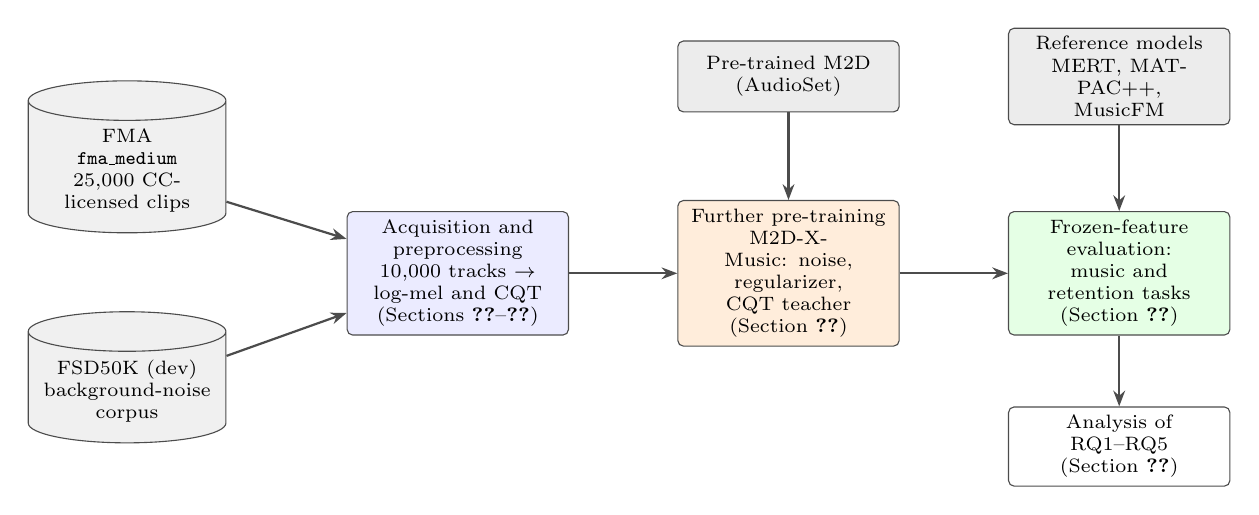
\begin{tikzpicture}
  \node[m5data] (fma) at (0,2.3) {FMA\\\texttt{fma\_medium}\\25,000 CC-licensed clips};
  \node[m5data] (fsd) at (0,-0.5) {FSD50K (dev)\\background-noise\\corpus};
  \node[m5proc] (prep) at (4.2,1.0) {Acquisition and\\preprocessing\\10,000 tracks $\rightarrow$\\log-mel and CQT\\(Sections~\ref{sec:m5-acq}--\ref{sec:m5-prep})};
  \node[m5ref] (base) at (8.4,3.5) {Pre-trained M2D\\(AudioSet)};
  \node[m5train] (pt) at (8.4,1.0) {Further pre-training\\M2D-X-Music: noise,\\regularizer, CQT teacher\\(Section~\ref{sec:m5-frame})};
  \node[m5eval] (ev) at (12.6,1.0) {Frozen-feature\\evaluation: music and\\retention tasks\\(Section~\ref{sec:m5-eval})};
  \node[m5ref] (ref) at (12.6,3.5) {Reference models\\MERT, MATPAC++,\\MusicFM};
  \node[m5box] (ana) at (12.6,-1.2) {Analysis of\\RQ1--RQ5\\(Section~\ref{sec:m5-rq})};
  \draw[m5arrow] (fma) -- (prep);
  \draw[m5arrow] (fsd) -- (prep);
  \draw[m5arrow] (prep) -- (pt);
  \draw[m5arrow] (base) -- (pt);
  \draw[m5arrow] (pt) -- (ev);
  \draw[m5arrow] (ref) -- (ev);
  \draw[m5arrow] (ev) -- (ana);
\end{tikzpicture}}
\caption[Overview of the proposed methodology]{Overview of the proposed methodology. A 10,000-track subset of FMA and a background-noise corpus are converted into the input format of the pre-trained M2D model. The model is further pre-trained with the M2D-X-Music objective. The resulting checkpoints and the reference models are then compared on music and retention tasks with frozen features.}
\label{fig:m5-overview}
\end{figure}


\section{Methodological Foundations}
\label{sec:m5-foundations}
This section reviews the work on which the methodology builds and states, for each source, what is adopted and what is deliberately left out. Table~\ref{tab:m5-decisions} at the end of the section collects these decisions.

\subsection{Masked Latent Prediction and M2D}
Masked prediction teaches an encoder to infer hidden parts of an input from the visible parts. Masked autoencoders reconstruct the hidden input values, first for images~\cite{ref:He:2022mae} and then for audio spectrograms~\cite{ref:Huang:2022audiomae}, so the learning signal depends partly on low-level detail. Methods that predict targets produced by a separate network instead avoid this dependence: BYOL~\cite{ref:Grill:2020byol}, data2vec~\cite{ref:Baevski:2022data2vec} and I-JEPA~\cite{ref:Assran:2023ijepa} regress the continuous latents of a slowly updated target network, and BEATs~\cite{ref:Chen:2023beats} predicts discrete labels from an acoustic tokenizer. Masked Modeling Duo (M2D)~\cite{ref:Niizumi:2023m2d,ref:Niizumi:2024m2dx} applies this idea to audio spectrograms with one distinguishing choice: the target network encodes \emph{only the masked patches}, so the target does not carry information about the visible patches that the online network could exploit, and both networks are encouraged to model the input.

The released M2D model~\cite{ref:M2DGit} takes a log-mel spectrogram of 6~s of audio at 16~kHz with 80 mel bins (80$\times$608 frames) and splits it into $16\times16$ patches, giving $N_F=5$ frequency positions and $N_T=38$ time positions, that is, $N=190$ patches. A vanilla ViT-Base encoder~\cite{ref:Dosovitskiy:2021vit} with 768-dimensional tokens and about 86~M parameters encodes the visible 30\,\% of the patches. A shallow transformer predictor, taken from the MAE decoder, receives the encoded visible patches together with shared learnable mask tokens and predicts the representations of the masked patches. The target encoder is an exponential moving average (EMA) of the online encoder. The model was pre-trained on AudioSet~\cite{ref:Gemmeke:2017audioset} (2,005,132 clips, 5,569~h) for 300 epochs with an effective batch size of 2,048~\cite{ref:Niizumi:2024m2dx}, and it achieved top-level linear-evaluation results across environmental, speech and music tasks. Related members of the family add an unsupervised classification objective (MATPAC~\cite{ref:Quelennec:2025matpac}) or multiple prediction hypotheses (MATPAC++~\cite{ref:Quelennec:2025matpacpp}), and M2D-CLAP aligns the representation with text~\cite{ref:Niizumi:2024m2dclap}. M2D is chosen as the base model of this study for three practical reasons: the code and the AudioSet weights are public~\cite{ref:M2DGit}, an official recipe for further pre-training exists, and its ViT-Base encoder is small enough for a single 16~GB GPU.

\subsection{Specializing a General Model: M2D-X}
M2D-X extends M2D to learn representations specialized to an application $X$ whose data are scarce and differ from the pre-training distribution~\cite{ref:Niizumi:2024m2dx}. It adds three ingredients. First, background noise from another corpus is mixed into the input of M2D. This acts as data augmentation, which matters because masked prediction normally needs large datasets~\cite{ref:Xie:2023datascaling}, and, because an additional network sees the clean signal, it forms a denoising task. Second, an \emph{offline network} receives the clean input and provides an additional training signal through a configurable loss, which can be supervised labels, the features of a domain model (distillation), or the features of the original pre-trained model (regularization). Third, the total loss is a weighted sum of the M2D loss and the offline loss. The earlier speech variant, M2D for Speech, distilled HuBERT features while denoising and reached results close to HuBERT on several speech tasks~\cite{ref:Niizumi:2023m2ds,ref:Hsu:2021hubert}.

The evidence most relevant to this project comes from the ICBHI 2017 respiratory-sound task, where only 539 training recordings (about 5.5~h for the whole database) were available~\cite{ref:Niizumi:2024m2dx}. The AudioSet model (a variant with $16\times4$ patches and 2-s inputs) scored 61.93 on the task metric. Further pre-training with the M2D loss alone and no background noise \emph{lowered} the score to 61.17, indicating overfitting to the small corpus. Adding background noise (mixing ratio 0.3) raised it to 62.73, and the full M2D-X, which adds the frozen-teacher regularizer, reached 63.29. The training list was replicated to 10,000 samples per epoch, 600 epochs were run with an effective batch size of 128 on a single 24~GB GPU, with the stated aim of completing pre-training within a day. The authors' guide~\cite{ref:M2DGit} states that this procedure suits application datasets of fewer than about 10,000 samples and that an effective batch size of 128 with 600 epochs worked for 10,000 samples. The 10,000-track budget of this project therefore sits at the upper end of the regime the recipe was designed for, which makes it a natural, low-risk starting point.

\subsection{Music-Specific Self-Supervised Models}
\paragraph{MERT.} MERT~\cite{ref:Li:2024mert} follows HuBERT-style masked prediction on raw audio with two teachers. The \emph{acoustic teacher} supplies discrete targets, obtained either by K-means on log-mel and chroma features or from the residual vector quantization codes of EnCodec~\cite{ref:Defossez:2023encodec}. The \emph{musical teacher} is a linear head on the encoder output that regresses the constant-Q transform (CQT)~\cite{ref:Brown:1991cqt} of the audio with a mean-squared-error loss, and the total loss is $\alpha\mathcal{L}_{H}+\mathcal{L}_{\mathrm{CQT}}$. The CQT has logarithmically spaced bins, so every octave has the same number of bins, which suits pitch and harmony. Adding the CQT term raised key-detection accuracy from 55.1 to 65.0 and GTZAN genre accuracy from 75.2 to 78.6 for the K-means teacher, and from 60.5 to 63.2 and from 72.8 to 77.2 for the RVQ teacher~\cite{ref:Li:2024mert}. MERT also mixes short excerpts from the same batch into each clip (in-batch noise mixup) with probability 0.5 in its final setting. Its official implementation computes the CQT magnitude with nnAudio~\cite{ref:Cheuk:2020nnaudio} using 84 bins at 12 bins per octave starting at 32.7~Hz~\cite{ref:MERTGit}, which is the configuration adopted here for the musical teacher. The base model was trained on about 1,000~h of music in the paper and on 160,000~h for the 330~M-parameter model~\cite{ref:Li:2024mert}; the public MERT-v1-95M checkpoint used in this study was trained on 20,000~h~\cite{ref:MERTCard}.

\paragraph{MusicFM and MuQ.} MusicFM~\cite{ref:Won:2024musicfm} adapts the BEST-RQ idea~\cite{ref:Chiu:2022bestrq} to music: targets are produced by a frozen random projection and a random codebook applied to normalized log-mel features, and a Conformer is trained to predict them. A variant trained on the whole FMA (about 8,000~h) scored below the variant trained on a 160,000-h in-house corpus on most downstream tasks, which the authors attribute to scale and to the crowd-sourced nature of FMA~\cite{ref:Won:2024musicfm}. MuQ~\cite{ref:Zhu:2025muq} predicts Mel-RVQ tokens and reports that it outperforms earlier self-supervised music models with only about 900~h of open-source pre-training data. These two models show that the FMA corpus is usable but not ideal, and that the choice of target matters more than its sophistication; they are used as reference models and their target definitions are not adopted, because both require pre-training from scratch.

\paragraph{MATPAC and MATPAC++.} MATPAC combines masked latent prediction with a DINO-style unsupervised classification objective~\cite{ref:Caron:2021dino}, with total loss $(1-\alpha)\mathcal{L}_{\mathrm{cls}}+\alpha\mathcal{L}_{\mathrm{pred}}$ and $\alpha=0.5$~\cite{ref:Quelennec:2025matpac}. MATPAC++ replaces the single prediction by several hypotheses selected with annealed multiple choice learning~\cite{ref:Perera:2024annealed,ref:Quelennec:2025matpacpp}. The finding that matters here is the effect of domain-specific training. When MATPAC++ was trained only on music (about 0.9~M Million Song Dataset samples plus about 0.18~M web-radio samples, roughly 30~h on four H100 GPUs for 6-s segments), its average over eight music tasks rose from 47.2 to 47.9 compared with training on AudioSet, a gain of 0.7 points~\cite{ref:Quelennec:2025matpacpp}. In the same table the AudioSet-trained M2D averages 46.3 against 44.2 for MERT, although the MERT scores were taken from its paper and the protocols are not identical. In short, general-audio models are already strong on music tasks, and large-scale music-only training adds little. This is the observation that motivates studying whether a \emph{small, cheap} music-specific step can recover a comparable increment.

\subsection{Further Pre-training, Forgetting and Regularization}
Continuing self-supervised pre-training on domain data is an established idea. In language modeling, domain-adaptive pre-training improves downstream tasks in both high- and low-resource settings~\cite{ref:Gururangan:2020dsp}. In speech, adding unlabeled in-domain data to pre-training reduces most of the gap caused by domain shift~\cite{ref:Hsu:2021robustw2v2}. The risks are equally well documented. Vision transformers further pre-trained on small target data overfit, which motivates distilling from a teacher that was itself further pre-trained~\cite{ref:Lee:2023selfdistill}. For audio, SONAR continues pre-training BEATs on domain data and compares it with direct continual pre-training that resumes the original objective unchanged~\cite{ref:Zhang:2025sonar}. On FMA-derived data of 30,000 to 50,000 segments, direct continuation reduced the frozen-feature GTZAN F1 score from 86.0 to 76.0 and lowered the AudioSet tagging mAP from 34.8 to 14.7, whereas SONAR, which adds distillation-based regularization and data sampling, raised GTZAN to 88.0 and kept the mAP at 34.7~\cite{ref:Zhang:2025sonar}. Another study with M2D found that, for narrow and small respiratory datasets, models pre-trained on diverse general audio beat models trained on the domain alone, and that further pre-training on a combination of general and domain data improved results~\cite{ref:Niizumi:2025resp}. The frozen-teacher term of M2D-X is closely related to learning without forgetting~\cite{ref:Li:2018lwf} and knowledge distillation~\cite{ref:Hinton:2015distill}, and it avoids the parameter-importance estimates required by elastic weight consolidation~\cite{ref:Kirkpatrick:2017ewc}. These studies jointly imply that naive continuation should be treated as a control that may fail, and that retention of general ability must be measured, not assumed.

\subsection{Design Decisions Derived from the Literature}
Table~\ref{tab:m5-decisions} summarizes, source by source, which finding is used and which decision follows from it in this study.

\begin{table}[!t]
\centering
\caption[Literature findings and the design decisions they lead to]{Literature findings and the design decisions they lead to.}
\label{tab:m5-decisions}
\small\singlespacing
\begin{tabularx}{\linewidth}{>{\raggedright\arraybackslash}p{2.7cm}>{\raggedright\arraybackslash}X>{\raggedright\arraybackslash}X}
\toprule
\textbf{Source} & \textbf{Finding used} & \textbf{Decision in this study}\\
\midrule
M2D, M2D-X~\cite{ref:Niizumi:2023m2d,ref:Niizumi:2024m2dx} & Latent prediction of masked patches; public AudioSet weights and further pre-training code; recipe for fewer than about 10,000 samples & Start from the AudioSet checkpoint with 80$\times$608 input, $16\times16$ patches and masking ratio 0.7; keep its loss as the base objective\\
M2D-X noise and regularizer~\cite{ref:Niizumi:2024m2dx} & Naive further pre-training degraded the score; noise and a frozen original-model teacher recovered and exceeded it & Use background noise ($\eta=0.3$) and the original M2D as frozen offline teacher; keep naive and partial variants as controls\\
MERT~\cite{ref:Li:2024mert} & A CQT-regression musical teacher improves key detection and genre classification; in-batch mixup helps the RVQ variant & Add a CQT teacher (84 bins) through the offline branch with weight 1; do not train an acoustic tokenizer\\
MATPAC, MATPAC++~\cite{ref:Quelennec:2025matpac,ref:Quelennec:2025matpacpp} & Music-only pre-training at scale adds about 0.7 points over AudioSet training; public checkpoints & Use their checkpoints as references; do not add the classification head or multiple hypotheses\\
MusicFM, MuQ~\cite{ref:Won:2024musicfm,ref:Zhu:2025muq} & FMA-only training trails a larger corpus; about 900~h of open data is enough for competitive results & Use as references with matched or larger data; do not adopt quantizer targets\\
Domain-adaptive pre-training, SONAR~\cite{ref:Gururangan:2020dsp,ref:Zhang:2025sonar,ref:Lee:2023selfdistill} & Naive continuation can hurt and forget; regularization and replay of general data help & Measure retention on environmental-sound tasks and report a forgetting score\\
FMA~\cite{ref:Defferrard:2017fma} & Creative Commons audio; 30-s clips; artist-filtered train, validation and test splits; curated medium subset & Sample from the training split of the medium subset only; cap tracks per artist; use no genre labels for pre-training\\
EVAR, MARBLE, HEAR~\cite{ref:M2DGit,ref:EVARGit,ref:Yuan:2023marble,ref:Turian:2022hear} & Frozen-feature linear probing is the common protocol for comparing audio representations & Evaluate every model with the same linear-probe protocol\\
\bottomrule
\end{tabularx}
\end{table}

\section{Research Questions and Hypotheses}
\label{sec:m5-rq}
The study is organized around five questions. Each is paired with a hypothesis that can be contradicted by the planned measurements. The arms and metrics named below are defined in Sections~\ref{sec:m5-design} and~\ref{sec:m5-eval}.
\begin{itemize}
  \item \textbf{RQ1.} Does further pre-training of the AudioSet-pretrained M2D on about 83~h of FMA music improve its frozen-feature performance on music tasks? \emph{H1:} the full recipe (A4) improves the average music score over the unmodified model (A0), whereas naive continuation (A1) does not.
  \item \textbf{RQ2.} Which parts of M2D-X are needed on music data? \emph{H2:} the order of the music score is A1 $<$ A2 $<$ A3, that is, background noise and the frozen-teacher regularizer each add a gain, as in the respiratory-sound study.
  \item \textbf{RQ3.} Does a CQT musical teacher add value beyond M2D-X? \emph{H3:} A4 exceeds A3 on pitch-related tasks (NSynth pitch) by more than the probe-seed uncertainty, and is not worse elsewhere.
  \item \textbf{RQ4.} How much of the gap to music-specific models does the cheap step close, and is general-audio ability kept? \emph{H4:} the best arm closes a clearly positive fraction of the gap to the public MERT checkpoints and loses less than 1 point of average environmental-sound accuracy (a tolerance fixed in advance), while a gap to the larger, longer-trained references may remain.
  \item \textbf{RQ5.} How does the benefit depend on the number of FMA tracks? \emph{H5:} the gain increases from 1,000 to 10,000 tracks with diminishing returns, so that most of it is reached before 10,000 tracks.
\end{itemize}
An outcome contradicting a hypothesis, such as no benefit of the CQT teacher or a collapse of retention, is a valid finding and will be reported as such.

\section{Dataset Acquisition}
\label{sec:m5-acq}
This section describes where the pre-training audio comes from, which part of it is eligible, and how the 10,000-sample subset is drawn. Throughout this report a \emph{sample} is one 30-s FMA clip, that is, one track, so 10,000 samples correspond to 10,000 tracks or about 83.3~h of music. This is about 1.5\,\% of the 5,569~h of AudioSet on which M2D was trained.

\subsection{Choice of Corpus}
The pre-training corpus must satisfy five requirements: it can be obtained and used legally for research; it provides full-quality audio, not only derived features or links; its metadata identify artists and provide predefined splits, so that leakage can be controlled; it is small enough to download and process on one workstation; and it has been used in earlier music self-supervised work, so that results can be compared. The Free Music Archive (FMA)~\cite{ref:Defferrard:2017fma} meets all five requirements. Its audio is licensed under Creative Commons licenses chosen by the artists, the tracks are MP3 files, most of them stereo at 44.1~kHz and 320~kbit/s (263~kbit/s on average), and the metadata include artist identifiers and an official split with an artist filter. FMA has been used to pre-train MusicFM~\cite{ref:Won:2024musicfm}, it is part of the data of the public MERT-v0-public model according to its model card~\cite{ref:MERTCard}, and FMA-derived data were used for continual pre-training of BEATs~\cite{ref:Zhang:2025sonar}. The alternatives are less suitable: the Million Song Dataset does not distribute audio, AudioSet consists of links to online videos whose availability changes, which already makes published results hard to compare~\cite{ref:Quelennec:2025matpacpp}, and MagnaTagATune (32~kbit/s, 16~kHz mono) and GTZAN (about 1,000 clips with documented faults~\cite{ref:Sturm:2013gtzan}) are too small or too low in quality for pre-training and are used only as evaluation sets.

\subsection{Archives and Metadata}
FMA is distributed as one metadata archive (\texttt{fma\_metadata.zip}) and four audio archives that are nested subsets of one another~\cite{ref:Defferrard:2017fma,ref:FMAGit}. The metadata table \texttt{tracks.csv} describes all 106,574 tracks, with artist, album, genre, license, and the columns that give the subset and the official training, validation and test split of each track. In the medium, small and large subsets the audio of a track is a 30-s clip cut from the middle of the full track, or the whole track if it is shorter. The medium subset contains 25,000 clips with a single top-level genre each, selected according to the completeness of their metadata and their popularity in the hope of selecting tracks of higher quality; the small subset is the balanced selection of 1,000 clips from each of the eight most popular genres of the medium subset~\cite{ref:Defferrard:2017fma}. The splits are 80\,\%/10\,\%/10\,\% for training, validation and test, stratified by genre, with an artist filter so that every artist appears in only one split, and a track keeps the same split in every subset~\cite{ref:Defferrard:2017fma}.

\begin{table}[htbp]
\centering
\caption[FMA audio archives and their use in this study]{FMA audio archives and their use in this study. Sizes are those listed by the dataset maintainers~\cite{ref:FMAGit}; clip counts and genre counts are from the dataset paper~\cite{ref:Defferrard:2017fma}.}
\label{tab:m5-fma}
\small\singlespacing
\begin{tabularx}{\linewidth}{lrrrY}
\toprule
\textbf{Archive} & \textbf{Clips} & \textbf{Genres} & \textbf{Size (GiB)} & \textbf{Use in this study}\\
\midrule
\texttt{fma\_small} & 8,000 & 8 (balanced) & 7.2 & Audio contained in the medium archive; official test split used for in-domain genre evaluation\\
\texttt{fma\_medium} & 25,000 & 16 (unbalanced) & 22 & Source of the pre-training pool (training split only) and of the \texttt{fma\_small} evaluation clips\\
\texttt{fma\_large} & 106,574 & 161 & 93 & Not used (larger download, no additional split advantage)\\
\texttt{fma\_full} & 106,574 & 161 & 879 & Not used (untrimmed tracks)\\
\bottomrule
\end{tabularx}
\end{table}

The study downloads the metadata archive and the medium audio archive only, verifies the SHA-1 checksums published with the dataset, and unpacks the files. Because the small subset is contained in the medium subset, the single audio archive also supplies the clips for the in-domain evaluation.

\subsection{Eligibility Rules and Subset Selection}
A track enters the candidate list only if it satisfies all of the following rules.
\begin{enumerate}
  \item It belongs to the small or medium subset and to the \emph{training} split. Since the official splits are artist-filtered, no artist from the validation or test split contributes to pre-training, which prevents in-domain leakage into the FMA evaluation task. About 80\,\% of the 25,000 clips, that is, about 20,000 tracks, are expected to qualify; the exact count is recorded when the metadata are read.
  \item Its license field is present in the metadata.
  \item It passes the audio audit described in Section~\ref{sec:m5-prep}.
  \item At most $k=5$ tracks of the same artist are admitted. This limits the influence of prolific artists in a corpus with a long-tailed artist distribution.
\end{enumerate}
No genre label is used for selection, so the subset keeps the genre distribution of the medium subset, in which experimental music is under-represented~\cite{ref:Defferrard:2017fma}; the genre histogram of the chosen subset is reported so that this property is visible. Pre-training itself uses no labels at all.

Algorithm~\ref{alg:m5-select} fixes the selection. A seeded random permutation of the eligible tracks defines the order in which candidates are examined. The first 10,000 accepted tracks form the main subset, and shorter prefixes of the same list form the nested subsets with 1,000, 2,500 and 5,000 tracks, plus a 20,000-track extension if time allows. Using prefixes of one list means that all arms and all sizes draw on the same data, so a difference between two results cannot come from a different selection of tracks. Only the ordered list of track identifiers and the seed need to be stored to reproduce the subset.

\begin{algorithm}[htbp]
\caption{Seeded, artist-capped selection of nested pre-training subsets}
\label{alg:m5-select}
\KwData{metadata table $T$; seed $s$; artist cap $k$; sizes $n_1<n_2<\dots<n_J$}
\KwResult{ordered list $L$ and nested subsets $S_j=L[1..n_j]$; rejection log}
$E\leftarrow\{t\in T:\ t.\mathrm{subset}\in\{\mathrm{small},\mathrm{medium}\},\ t.\mathrm{split}=\mathrm{training},\ t.\mathrm{license}\neq\emptyset\}$\;
$\pi\leftarrow$ random permutation of $E$ generated with seed $s$\;
$L\leftarrow$ empty list; $\mathrm{count}[a]\leftarrow 0$ for every artist $a$\;
\ForEach{track $t$ in $\pi$, in order}{
  \If{$\mathrm{count}[t.\mathrm{artist}]<k$ \textbf{and} $\mathrm{Audit}(t)$ passes}{
    append $t$ to $L$\;
    $\mathrm{count}[t.\mathrm{artist}]\leftarrow\mathrm{count}[t.\mathrm{artist}]+1$\;
  }
  \lIf{$|L|=n_J$}{leave the loop}
}
\textbf{return} $L$, the subsets $S_j$, and the log of rejected tracks with their reasons\;
\end{algorithm}

\subsection{Background-Noise Corpus}
The denoising component of M2D-X needs a corpus of background sounds. The official recipe uses the FSD50K dataset~\cite{ref:Fonseca:2022fsd50k,ref:Niizumi:2024m2dx}, which contains 51,197 Freesound clips (108.3~h) under Creative Commons licenses, labeled with 200 classes of the AudioSet ontology. Only the development portion is used as noise, and the evaluation portion is left untouched. Because the ontology includes musical instruments, an optional ablation restricts the pool to clips that carry no music-related label, to test whether purely non-musical noise is a better distractor for music (Section~\ref{sec:m5-design}).

\subsection{Licensing and Ethics}
FMA tracks carry artist-chosen Creative Commons licenses that permit research use. Audio and the spectrograms derived from it are kept local and are not redistributed; only the list of track identifiers and the seed are published. The metadata contain only public artist information and no personal data. The CC-BY-NC license of the MERT weights~\cite{ref:MERTCard} is respected by using them for non-commercial comparison only.

\section{Data Preprocessing Pipeline}
\label{sec:m5-prep}
Figure~\ref{fig:m5-pipeline} shows the pipeline. Its guiding rule is that the audio must reach the model through exactly the same front-end as in the original pre-training, because a pre-trained encoder that is fed differently computed spectrograms suffers a distribution shift that would be confounded with the effect under study.

\begin{figure}[htbp]
\centering
\resizebox{\linewidth}{!}{%
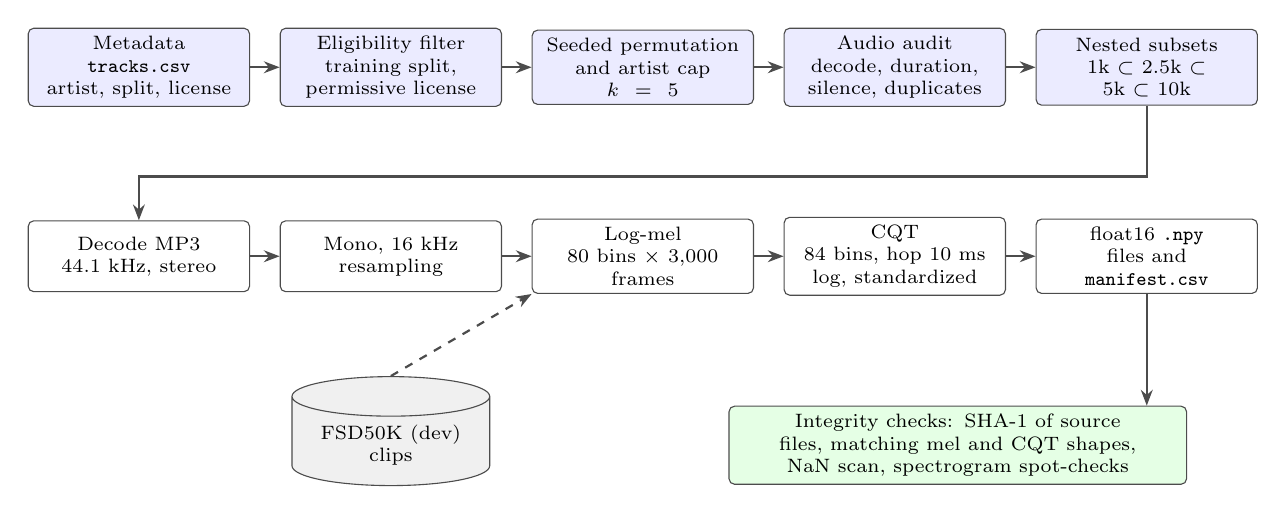
\begin{tikzpicture}
  \node[m5proc] (s1) at (0,3.0) {Metadata\\\texttt{tracks.csv}\\artist, split, license};
  \node[m5proc] (s2) at (3.2,3.0) {Eligibility filter\\training split,\\permissive license};
  \node[m5proc] (s3) at (6.4,3.0) {Seeded permutation\\and artist cap\\$k=5$};
  \node[m5proc] (s4) at (9.6,3.0) {Audio audit\\decode, duration,\\silence, duplicates};
  \node[m5proc] (s5) at (12.8,3.0) {Nested subsets\\1k $\subset$ 2.5k $\subset$\\5k $\subset$ 10k};
  \node[m5box] (c1) at (0,0.6) {Decode MP3\\44.1 kHz, stereo};
  \node[m5box] (c2) at (3.2,0.6) {Mono, 16 kHz\\resampling};
  \node[m5box] (c3) at (6.4,0.6) {Log-mel\\80 bins $\times$ 3,000\\frames};
  \node[m5box] (c4) at (9.6,0.6) {CQT\\84 bins, hop 10 ms\\log, standardized};
  \node[m5box] (c5) at (12.8,0.6) {float16 \texttt{.npy}\\files and\\\texttt{manifest.csv}};
  \node[m5data] (n1) at (3.2,-1.8) {FSD50K (dev)\\clips};
  \node[m5eval, text width=5.6cm] (chk) at (10.4,-1.8) {Integrity checks: SHA-1 of source files, matching mel and CQT shapes, NaN scan, spectrogram spot-checks};
  \draw[m5arrow] (s1) -- (s2);
  \draw[m5arrow] (s2) -- (s3);
  \draw[m5arrow] (s3) -- (s4);
  \draw[m5arrow] (s4) -- (s5);
  \draw[m5arrow] (s5.south) -- ++(0,-0.9) -| (c1.north);
  \draw[m5arrow] (c1) -- (c2);
  \draw[m5arrow] (c2) -- (c3);
  \draw[m5arrow] (c3) -- (c4);
  \draw[m5arrow] (c4) -- (c5);
  \draw[m5arrow, dashed] (n1.north) -- (c3.south west);
  \draw[m5arrow] (c5.south) -- (c5.south |- chk.north);
\end{tikzpicture}}
\caption[Data acquisition and preprocessing pipeline]{Data acquisition and preprocessing pipeline. The top row operates on metadata and audit results and fixes the ordered list of tracks. The bottom row converts the selected files with the same front-end that was used to pre-train M2D. The noise corpus passes through the log-mel stage only (dashed arrow).}
\label{fig:m5-pipeline}
\end{figure}


\subsection{Audit and Decoding}
Each candidate MP3 file is decoded before it is accepted. The FMA maintainers document corrupted or truncated tracks, tracks shorter than 30~s, and duplicates~\cite{ref:FMAGit}, so the audit applies four rejection rules.
\begin{enumerate}
  \item \textbf{Decoding failure:} the decoder reports an error or a truncated stream.
  \item \textbf{Duration:} the decoded signal is shorter than 10~s, so that several different 6.08-s windows cannot be cut from it.
  \item \textbf{Silence:} more than half of the frames have a power more than 60~dB below that of the loudest frame of the clip.
  \item \textbf{Duplication:} the track has the same normalized pair of artist identifier and title as an accepted track, or the same hash of the decoded 16-kHz waveform. The track with the lowest identifier is kept.
\end{enumerate}
Every rejection is logged with its reason, and the next candidate in the permutation takes the place of a rejected track (Algorithm~\ref{alg:m5-select}).

\subsection{Front-End}
The conversion script distributed with the M2D code (\texttt{wav\_to\_lms.py})~\cite{ref:M2DGit} is used without modification. It loads each file as a mono signal resampled to 16~kHz and computes a log-mel spectrogram with nnAudio~\cite{ref:Cheuk:2020nnaudio}. With the mel filter bank $H$ and the short-time Fourier transform $X$ of the waveform, each spectrogram entry is
\begin{equation}
x_{f,t}=\log\!\Big(\sum_{k}H_{f,k}\,\lvert X_{k,t}\rvert^{2}+\epsilon\Big),\qquad f=1,\dots,80,
\label{eq:m5-logmel}
\end{equation}
where $\epsilon$ is a small constant that avoids the logarithm of zero. Table~\ref{tab:m5-frontend} lists all parameters. Spectrograms are stored in half precision, which halves the disk space (about 4.8~GB for 10,000 clips of 3,000 frames) at a rounding error far below the standard deviation of the data, and they are cast to single precision when loaded.

\begin{table}[htbp]
\centering
\caption[Front-end and target parameters]{Front-end and target parameters. Values of the log-mel front-end and of the input geometry follow the released M2D model~\cite{ref:M2DGit,ref:Niizumi:2024m2dx}; the CQT settings follow the official MERT implementation~\cite{ref:MERTGit}, with the hop size changed to match the log-mel frame grid.}
\label{tab:m5-frontend}
\small\singlespacing
\begin{tabularx}{\linewidth}{>{\raggedright\arraybackslash}p{4.4cm}Y}
\toprule
\textbf{Item} & \textbf{Value}\\
\midrule
Audio decoding & Channel mean to mono, resampled to 16~kHz\\
STFT & Window and FFT size 400 samples (25~ms), hop 160 samples (10~ms)\\
Mel bands & 80 bands between 50~Hz and 8,000~Hz\\
Input window & 608 frames ($\approx$6.08~s); patches of $16\times16$; $N_F=5$, $N_T=38$, $N=190$ patches\\
Normalization & Mean $\mu_{\mathrm{AS}}=-7.1$ and standard deviation $\sigma_{\mathrm{AS}}=4.2$ of the AudioSet pre-training data\\
CQT target & Magnitude, 84 bins at 12 per octave from 32.7~Hz (C1) to about 3.95~kHz, hop 160 samples; logarithm, standardized per bin\\
Target token rate & Average over $P=16$ frames (160~ms) to match one patch step\\
\bottomrule
\end{tabularx}
\end{table}

\subsection{Cropping and Normalization}
At every visit, a random window of 608 frames is cut from the stored 30-s spectrogram, as in the official loader. A 30-s track contains about five non-overlapping windows, and random start positions give many more overlapping ones, so the 10,000 tracks supply a large number of distinct inputs even though the track count is small. The window is standardized as
\begin{equation}
\bar{x}=\frac{x-\mu_{\mathrm{AS}}}{\sigma_{\mathrm{AS}}},
\label{eq:m5-norm}
\end{equation}
with the AudioSet statistics of Table~\ref{tab:m5-frontend}, so that the pre-trained encoder initially sees inputs of the same scale as during its original pre-training. The official M2D-X code instead recomputes these statistics from the application data at run time. The deviation is deliberate: it removes one source of change at the start of training. The mean and standard deviation of the selected FMA subset are computed and reported so that the size of the shift is known, and training with the FMA statistics is kept as an optional ablation.

\subsection{Musical-Teacher Targets}
The musical teacher uses the constant-Q transform~\cite{ref:Brown:1991cqt}, whose center frequencies are spaced logarithmically,
\begin{equation}
f_k=f_{\min}\,2^{(k-1)/12},\qquad k=1,\dots,84,\quad f_{\min}=32.7~\mathrm{Hz},
\label{eq:m5-cqtfreq}
\end{equation}
so that every semitone has its own bin and the top bin lies at about 3.95~kHz, below the Nyquist frequency of 8~kHz. Let $C_{k,t}$ be the CQT magnitude computed with nnAudio on the same 16-kHz mono waveform and with the same hop of 160 samples as the log-mel spectrogram. The target is the log magnitude standardized per bin with the mean $m_k$ and standard deviation $s_k$ over the selected subset, followed by average pooling over the $P=16$ frames of each token time step $\tau$:
\begin{equation}
\tilde{c}_{k,t}=\frac{\log(C_{k,t}+\epsilon)-m_k}{s_k},\qquad
\bar{c}_{k,\tau}=\frac{1}{P}\sum_{t=(\tau-1)P+1}^{\tau P}\tilde{c}_{k,t}.
\label{eq:m5-cqttarget}
\end{equation}
The choices differ from MERT in three respects, each for a reason. MERT regresses the linear magnitude on masked frames at its own frame rate; here the logarithm and the per-bin standardization keep the target on a scale comparable to the log-mel input and avoid a regression dominated by a few loud low-frequency bins, and the pooling matches the 160-ms time step of an M2D token. The CQT is deterministic and needs no additional network, and nnAudio is already a dependency of the M2D front-end. Because the two transforms use the same hop and centered frames, the log-mel and CQT arrays of a clip have the same number of frames; if they differ by a frame because of padding, both are trimmed to the shorter, and one random start index is used to crop both.

\subsection{Storage, Manifest and Integrity Checks}
For each accepted track the pipeline writes one half-precision array for the log-mel spectrogram (about 4.8~GB for 10,000 clips) and one for the CQT (about 5.0~GB), and a row in a manifest file with the track identifier, artist identifier, file paths, frame counts, SHA-1 of the source file, audit outcome and split. The noise corpus is converted to log-mel arrays only. The following checks are run and their outcome is saved: the SHA-1 of every source file matches the published checksum; log-mel and CQT frame counts agree; no array contains NaN or infinite values; value ranges lie within a plausible interval of the normalized scale; and a gallery of 20 randomly chosen spectrograms is inspected by eye against the audio. The conversion is resumable and driven by one configuration file, so an interrupted run does not repeat finished tracks.

\section{Further Pre-training Framework}
\label{sec:m5-frame}
This section defines M2D-X-Music, the objective and the training procedure applied to the AudioSet-pretrained M2D. Figure~\ref{fig:m5-framework} shows the data flow.

\begin{figure}[htbp]
\centering
\resizebox{\linewidth}{!}{%
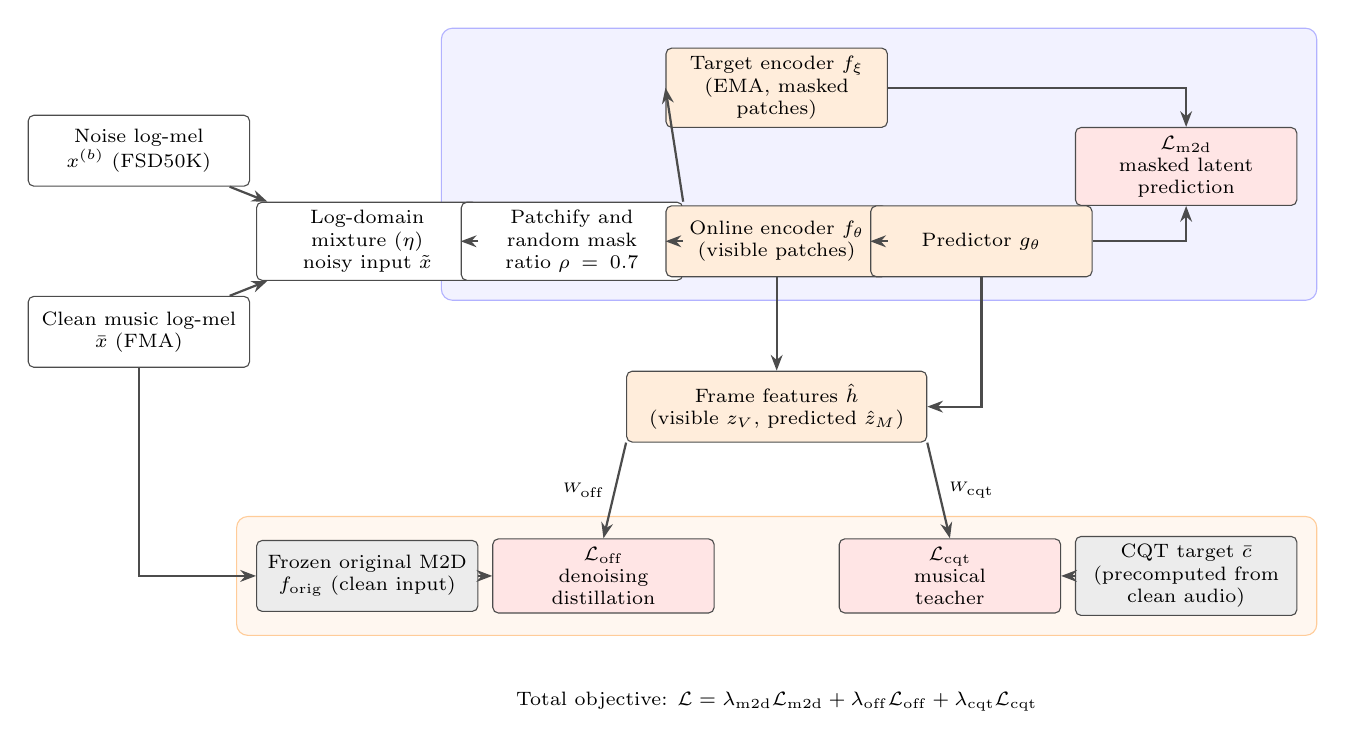
\begin{tikzpicture}
  \node[m5box] (xn) at (0,3.7) {Noise log-mel\\$x^{(b)}$ (FSD50K)};
  \node[m5box] (xc) at (0,1.4) {Clean music log-mel\\$\bar{x}$ (FMA)};
  \node[m5box] (mix) at (2.9,2.55) {Log-domain\\mixture ($\eta$)\\noisy input $\tilde{x}$};
  \node[m5box] (mask) at (5.5,2.55) {Patchify and\\random mask\\ratio $\rho=0.7$};
  \node[m5train] (tg) at (8.1,4.5) {Target encoder $f_\xi$\\(EMA, masked patches)};
  \node[m5train] (on) at (8.1,2.55) {Online encoder $f_\theta$\\(visible patches)};
  \node[m5train] (pr) at (10.7,2.55) {Predictor $g_\theta$};
  \node[m5box, fill=red!10] (lm) at (13.3,3.5) {$\mathcal{L}_{\mathrm{m2d}}$\\masked latent\\prediction};
  \node[m5train, text width=3.6cm] (hh) at (8.1,0.45) {Frame features $\hat{h}$\\(visible $z_V$, predicted $\hat{z}_M$)};
  \node[m5ref] (fo) at (2.9,-1.7) {Frozen original M2D\\$f_{\mathrm{orig}}$ (clean input)};
  \node[m5box, fill=red!10] (lo) at (5.9,-1.7) {$\mathcal{L}_{\mathrm{off}}$\\denoising\\distillation};
  \node[m5box, fill=red!10] (lc) at (10.3,-1.7) {$\mathcal{L}_{\mathrm{cqt}}$\\musical\\teacher};
  \node[m5ref] (cq) at (13.3,-1.7) {CQT target $\bar{c}$\\(precomputed from\\clean audio)};
  \draw[m5arrow] (xn) -- (mix);
  \draw[m5arrow] (xc) -- (mix);
  \draw[m5arrow] (mix) -- (mask);
  \draw[m5arrow] (mask) -- (on);
  \draw[m5arrow] (mask.north east) -- (tg.west);
  \draw[m5arrow] (on) -- (pr);
  \draw[m5arrow] (tg.east) -| (lm.north);
  \draw[m5arrow] (pr.east) -| (lm.south);
  \draw[m5arrow] (on) -- (hh);
  \draw[m5arrow] (pr.south) |- (hh.east);
  \draw[m5arrow] (xc.south) |- (fo.west);
  \draw[m5arrow] (fo) -- (lo);
  \draw[m5arrow] (hh.south west) -- node[left, font=\tiny] {$W_{\mathrm{off}}$} (lo.north);
  \draw[m5arrow] (hh.south east) -- node[right, font=\tiny] {$W_{\mathrm{cqt}}$} (lc.north);
  \draw[m5arrow] (cq) -- (lc);
  \node[font=\scriptsize, align=center] at (8.1,-3.3) {Total objective: $\mathcal{L}=\lambda_{\mathrm{m2d}}\mathcal{L}_{\mathrm{m2d}}+\lambda_{\mathrm{off}}\mathcal{L}_{\mathrm{off}}+\lambda_{\mathrm{cqt}}\mathcal{L}_{\mathrm{cqt}}$};
  \begin{scope}[on background layer]
    \node[fit=(mask)(tg)(on)(pr)(lm), fill=blue!5, draw=blue!30, rounded corners, inner sep=7pt] {};
    \node[fit=(fo)(lo)(lc)(cq), fill=orange!6, draw=orange!40, rounded corners, inner sep=7pt] {};
  \end{scope}
\end{tikzpicture}}
\caption[Architecture of the further pre-training framework]{Architecture of the further pre-training framework. The online and target networks receive the noisy input (top region), whereas the offline branch receives the clean input and its precomputed targets (bottom region). The frame features $\hat{h}$ are shared by the two offline losses through separate linear mappers $W_{\mathrm{off}}$ and $W_{\mathrm{cqt}}$. Only the online encoder $f_\theta$ is kept after pre-training.}
\label{fig:m5-framework}
\end{figure}


\subsection{Overview, Initialization and Alternatives Considered}
Training starts from the released checkpoint M2D/0.7 (80$\times$608 input, $16\times16$ patches, masking ratio 0.7)~\cite{ref:M2DGit}. The online encoder $f_\theta$, the predictor $g_\theta$ and the EMA target encoder $f_\xi$ are all initialized from this checkpoint, and a frozen copy $f_{\mathrm{orig}}$ of the original encoder serves as offline teacher. Two linear mappers, $W_{\mathrm{off}}$ and $W_{\mathrm{cqt}}$, are newly initialized. The online and target networks see the \emph{noisy} input, whereas the offline branch sees the \emph{clean} input and its precomputed targets. After pre-training only the online encoder is kept; its output features are what the evaluation of Section~\ref{sec:m5-eval} uses.

Four alternatives were considered and not adopted. Pre-training on FMA from scratch would answer a different question and is far beyond the single-GPU budget. Restricting updates to adapter or low-rank parameters would reduce forgetting but changes the model the study sets out to compare, and it is better left to later work. Distilling the features of a frozen MERT model is the exact analogue of the HuBERT distillation of M2D for Speech, but it needs a second, 24-kHz raw-audio branch and a second data format; it is kept as an optional extension. Replacing the objective by quantizer targets in the style of MusicFM or MuQ would require training the whole model again.

\subsection{Masked Latent Prediction on Noisy Music}
The standardized window is cut into $N=N_FN_T=190$ patches. A random subset $\mathcal{M}$ of $|\mathcal{M}|=\mathrm{round}(\rho N)=133$ patches is masked with $\rho=0.7$, and the remaining 57 patches form the visible set $\mathcal{V}$. The online encoder maps the visible patches to $z_{\mathcal V}=f_\theta(\tilde{x}_{\mathcal V})$, and the predictor, given mask tokens $m$ and positional encodings $p$, predicts all token representations,
\begin{equation}
\hat{z}=g_\theta\big(\mathrm{concat}(z_{\mathcal V},m)+p\big),
\label{eq:m5-pred}
\end{equation}
of which only the masked ones, $\hat{z}_{\mathcal M}$, are used in the loss. The target encoder receives the masked patches only, $z_{\mathcal M}=f_\xi(\tilde{x}_{\mathcal M})$, and its output is standardized to zero mean and unit variance, giving $\tilde{z}_{\mathcal M}$. The loss is the mean squared error between the $\ell_2$-normalized prediction and target,
\begin{equation}
\mathcal{L}_{\mathrm{m2d}}=\frac{1}{|\mathcal{M}|}\sum_{j\in\mathcal{M}}\left\lVert\frac{\hat{z}_j}{\lVert\hat{z}_j\rVert_2}-\frac{\tilde{z}_j}{\lVert\tilde{z}_j\rVert_2}\right\rVert_2^{2}
=\frac{1}{|\mathcal{M}|}\sum_{j\in\mathcal{M}}\left(2-2\,\frac{\langle\hat{z}_j,\tilde{z}_j\rangle}{\lVert\hat{z}_j\rVert_2\,\lVert\tilde{z}_j\rVert_2}\right).
\label{eq:m5-m2d}
\end{equation}
No gradient flows into the target encoder. Its parameters follow the online encoder by an exponential moving average,
\begin{equation}
\xi\leftarrow\tau_k\,\xi+(1-\tau_k)\,\theta,\qquad
\tau_k=\tau_0+(\tau_1-\tau_0)\,\frac{k}{K},
\label{eq:m5-ema}
\end{equation}
where $k$ is the optimizer step, $K$ the total number of steps, $\tau_0=0.99995$ and $\tau_1=0.99999$.

\subsection{Background Noise and Denoising}
To build the noisy input, a window of the noise corpus is mixed with the music window in the power domain, after the mean log level of each corpus has been removed so that the two sources start at comparable levels. With the music log-mel window $x^{(m)}$, the noise window $x^{(b)}$, their corpus means $\mu_m$ and $\mu_b$, and the mixing ratio $\eta$,
\begin{equation}
x_{\mathrm{mix}}=\log\Big((1-\eta)\exp\big(x^{(m)}-\mu_m\big)+\eta\exp\big(x^{(b)}-\mu_b\big)\Big),\qquad
\tilde{x}=\frac{x_{\mathrm{mix}}}{\sigma_{\mathrm{AS}}},
\label{eq:m5-mix}
\end{equation}
which is the mixing rule of M2D-X~\cite{ref:Niizumi:2024m2dx} followed by the same scale normalization as in Equation~\ref{eq:m5-norm}. Here $\mu_m$ is the AudioSet mean $\mu_{\mathrm{AS}}$ of Table~\ref{tab:m5-frontend} and $\mu_b$ is the mean of the noise corpus. The noise windows are drawn without replacement by cycling through a shuffled list of the corpus, and short noise clips are repeated to fill the window. The ratio is fixed at $\eta=0.3$ in the arms that use noise, the value of the respiratory-sound recipe~\cite{ref:Niizumi:2024m2dx}. Without a second view, the noise would only be an augmentation; the denoising character arises because the offline losses below are computed against the \emph{clean} signal, so the encoder is asked to produce features that describe the music underneath the noise.

\subsection{Frozen-Teacher Regularization}
Both offline losses act on frame-level features. Let $\hat{Z}$ be the grid of $N_F\times N_T$ token representations in which the visible positions hold the encoder outputs $z_{\mathcal V}$ and the masked positions hold the predictions $\hat{z}_{\mathcal M}$. The feature of time step $\tau$ is the concatenation over the $N_F$ frequency positions,
\begin{equation}
\hat{h}_\tau=\mathrm{concat}\big(\hat{Z}_{1,\tau},\dots,\hat{Z}_{N_F,\tau}\big)\in\mathbb{R}^{N_FD},\qquad N_FD=5\times768=3840,
\label{eq:m5-frame}
\end{equation}
which is the same layout as the 3,840-dimensional frame features used in the linear evaluation of M2D~\cite{ref:M2DGit}. The frozen original encoder $f_{\mathrm{orig}}$ processes the \emph{clean} window with all patches visible and gives the target features $y^{\mathrm{off}}_\tau\in\mathbb{R}^{3840}$. The regularization loss compares them after a linear map,
\begin{equation}
\mathcal{L}_{\mathrm{off}}=\frac{1}{N_T}\sum_{\tau=1}^{N_T}\left\lVert\frac{W_{\mathrm{off}}\hat{h}_\tau+b_{\mathrm{off}}}{\lVert W_{\mathrm{off}}\hat{h}_\tau+b_{\mathrm{off}}\rVert_2}-\frac{y^{\mathrm{off}}_\tau}{\lVert y^{\mathrm{off}}_\tau\rVert_2}\right\rVert_2^{2}.
\label{eq:m5-off}
\end{equation}
This term anchors the features of the adapted model to those of the original model on clean inputs, in the manner of learning without forgetting~\cite{ref:Li:2018lwf}, while the first term moves them towards the music distribution. In the speech variant the same mechanism distils a domain model; here the teacher is the model itself, so the term is a regularizer, as in the respiratory-sound experiments~\cite{ref:Niizumi:2024m2dx}.

\subsection{Musical Teacher}
The musical teacher adds a second offline task on the same frame features. A linear mapper predicts the pooled CQT target of Equation~\ref{eq:m5-cqttarget},
\begin{equation}
\mathcal{L}_{\mathrm{cqt}}=\frac{1}{N_T\,K_c}\sum_{\tau=1}^{N_T}\left\lVert W_{\mathrm{cqt}}\hat{h}_\tau+b_{\mathrm{cqt}}-\bar{c}_\tau\right\rVert_2^{2},\qquad K_c=84.
\label{eq:m5-cqt}
\end{equation}
Because $\hat{h}_\tau$ is built from encoder outputs at visible positions and from predictor outputs at masked positions, the term has two roles at once: it asks the encoder to recover the clean pitch content from noisy visible patches, and it asks the predictor to infer the pitch content of hidden regions. This differs from MERT, where the CQT is regressed on masked positions of a single network, and it keeps the M2D-X convention that offline losses act on all frames. Since the target is standardized, the initial value of the loss is of the order of one, comparable to the other two terms, and the weight $\lambda_{\mathrm{cqt}}=1$ follows MERT's finding that a unit weight worked best among 1, 2 and 5~\cite{ref:Li:2024mert}.

\subsection{Joint Objective and Optimization}
The full objective is the weighted sum
\begin{equation}
\mathcal{L}=\lambda_{\mathrm{m2d}}\,\mathcal{L}_{\mathrm{m2d}}+\lambda_{\mathrm{off}}\,\mathcal{L}_{\mathrm{off}}+\lambda_{\mathrm{cqt}}\,\mathcal{L}_{\mathrm{cqt}}.
\label{eq:m5-total}
\end{equation}
The experimental arms of Section~\ref{sec:m5-design} differ only in $\eta$, $\lambda_{\mathrm{off}}$ and $\lambda_{\mathrm{cqt}}$; all other settings are identical and are listed in Table~\ref{tab:m5-hparams}. They follow the official M2D-X recipe~\cite{ref:M2DGit,ref:Niizumi:2024m2dx} with AdamW~\cite{ref:Loshchilov:2019adamw}. The learning rate is scaled with the effective batch size $B_{\mathrm{eff}}$ by the rule of the code base,
\begin{equation}
\mathrm{lr}=\mathrm{blr}\cdot\frac{B_{\mathrm{eff}}}{256}=3\times10^{-4}\cdot\frac{128}{256}=1.5\times10^{-4}.
\label{eq:m5-lr}
\end{equation}
The effective batch size is kept at 128 even though the micro-batch is smaller, because the EMA update is applied once per optimizer step, so the number of steps affects the target network; the guide of the authors stresses that the effective batch size matters~\cite{ref:M2DGit}. Algorithm~\ref{alg:m5-train} gives the procedure.

\begin{table}[htbp]
\centering
\caption[Fixed settings of the further pre-training runs]{Fixed settings of the further pre-training runs. Settings in the upper part follow the released M2D model and the M2D-X recipe; the lower part are the choices made for this study.}
\label{tab:m5-hparams}
\small\singlespacing
\begin{tabularx}{\linewidth}{>{\raggedright\arraybackslash}p{4.0cm}Y}
\toprule
\textbf{Item} & \textbf{Setting}\\
\midrule
Initial weights & M2D/0.7 (\texttt{m2d\_vit\_base-80x608p16x16-221006-mr7}): online encoder, predictor and target encoder\\
Network & ViT-Base encoder, 768-dimensional tokens, about 86~M parameters; MAE-style predictor\\
Input and masking & 80$\times$608 log-mel window, $16\times16$ patches ($N=190$), masking ratio 0.7 (57 visible, 133 masked)\\
Optimizer & AdamW with $\beta=(0.9,0.95)$, weight decay 0.05, gradient-norm clipping at 3.0\\
Learning rate & Base $3\times10^{-4}$ scaled to $1.5\times10^{-4}$; 24 warm-up epochs; cosine decay to zero\\
EMA decay & Linear from 0.99995 to 0.99999 over training\\
\midrule
Epochs and data per epoch & 600 epochs of 10,000 virtual samples, that is, 6.0~M sample views and 46,875 optimizer steps\\
Batch & Micro-batch 32, gradient accumulation 4, effective batch 128\\
Noise & FSD50K development clips, $\eta=0.3$ in arms with noise\\
Loss weights & $\lambda_{\mathrm{m2d}}=1$; $\lambda_{\mathrm{off}}\in\{0,1\}$; $\lambda_{\mathrm{cqt}}\in\{0,1\}$\\
Precision and hardware & Mixed precision on one RTX A4000 (16~GB)\\
Checkpoints & Saved every 100 epochs; epoch 600 is the reported checkpoint\\
\bottomrule
\end{tabularx}
\end{table}

\begin{algorithm}[htbp]
\caption{Further pre-training with the M2D-X-Music objective}
\label{alg:m5-train}
\KwData{initial weights $(\theta_0,\xi_0)$; frozen teacher $f_{\mathrm{orig}}$; music list $\mathcal{D}$ with log-mel and CQT arrays; noise list $\mathcal{B}$; $\eta$, $\lambda_{\mathrm{m2d}}$, $\lambda_{\mathrm{off}}$, $\lambda_{\mathrm{cqt}}$; epochs $E$; epoch size $n$; micro-batch $b$; accumulation $a$}
\KwResult{further pre-trained encoder $f_\theta$}
$\theta\leftarrow\theta_0$; $\xi\leftarrow\xi_0$; initialize $W_{\mathrm{off}}$, $W_{\mathrm{cqt}}$\;
repeat $\mathcal{D}$ until the epoch list $\mathcal{D}_n$ has $n$ entries\;
\For{$e=1$ \KwTo $E$}{
  shuffle $\mathcal{D}_n$\;
  \ForEach{micro-batch of $b$ clips}{
    \ForEach{clip $i$ in the micro-batch}{
      draw one start index; crop 608 frames of the log-mel array and of the CQT array at that index\;
      take the next crop from the shuffled noise list $\mathcal{B}$ and form $\tilde{x}_i$ with Equation~\ref{eq:m5-mix}\;
    }
    draw random masks; compute $\mathcal{L}_{\mathrm{m2d}}$ with Equations~\ref{eq:m5-pred} and \ref{eq:m5-m2d}\;
    build $\hat{h}$ (Equation~\ref{eq:m5-frame}); compute $y^{\mathrm{off}}$ from the clean window with $f_{\mathrm{orig}}$ without gradient\;
    compute $\mathcal{L}_{\mathrm{off}}$ and $\mathcal{L}_{\mathrm{cqt}}$ (Equations~\ref{eq:m5-off} and \ref{eq:m5-cqt}); form $\mathcal{L}$ (Equation~\ref{eq:m5-total})\;
    backpropagate $\mathcal{L}/a$ into $\theta$, $W_{\mathrm{off}}$, $W_{\mathrm{cqt}}$\;
    \If{$a$ micro-batches have been accumulated}{
      clip the gradient norm; apply an AdamW step with the scheduled learning rate\;
      update $\xi$ with Equation~\ref{eq:m5-ema}\;
    }
  }
  \lIf{$e$ is a multiple of 100}{save a checkpoint of $f_\theta$}
}
\textbf{return} $f_\theta$\;
\end{algorithm}

\subsection{Compute and Memory Budget}
One run processes $600\times10{,}000=6.0$ million sample views, which is about 1\,\% of the roughly 600 million views of the original AudioSet pre-training (300 epochs of about two million clips). The respiratory-sound run of the authors, which had the same number of views, used one RTX 3090 Ti with 24~GB, 2-s inputs and $16\times4$ patches (250 patches per input), and aimed to finish pre-training within a day~\cite{ref:Niizumi:2024m2dx}. The window of this study has 190 patches, but the RTX A4000 has less memory and, to our knowledge, lower throughput, so the time per run is not known in advance: the budget assumes a run of the order of one day and is to be confirmed by a pilot of a few epochs before the main runs. The micro-batch of 32 is the setting that the authors give for smaller GPUs~\cite{ref:M2DGit}. If it does not fit into 16~GB, the micro-batch is halved and the accumulation doubled, which leaves the effective batch size of 128 unchanged. If the throughput is lower than expected, the number of epochs is reduced for \emph{all} arms alike, and the intermediate checkpoints saved every 100 epochs make the effect of the shorter schedule visible in the data.

\section{Experimental Design}
\label{sec:m5-design}
The experiments fall into three groups: reference models that are only evaluated, a small set of further pre-training \emph{arms} that differ in one factor at a time, and runs that vary the number of FMA tracks. All pre-training runs are compute-matched, that is, each processes the same number of sample views.

\subsection{Reference Models}
Table~\ref{tab:m5-refs} lists the models against which the further pre-trained checkpoints are compared. They are chosen to separate the effect of data volume from the effect of the objective. MERT-v1-95M and MERT-v0-public have a parameter count similar to that of the M2D encoder (95~M against 86~M) but were trained from scratch on about 20,000~h and about 900~h of music, which is roughly 240 and 11 times the 83~h of FMA used here, and MusicFM-FMA shows what training from scratch on the whole of FMA achieves. Reference models are never fine-tuned or further trained. For transformer references whose layers differ in quality, features of all layers are extracted and the best layer is chosen per task on the validation split; this is a favorable setting for the references and therefore a conservative one for the claims of this study. For the M2D family the final-layer features with the 3,840-dimensional frame layout of the original linear evaluation are used. Audio is resampled to the rate of each model and cut into windows of the context length of the model (5~s for MERT), and the segment embeddings are averaged over time.

\begin{table}[htbp]
\centering
\caption[Reference models]{Reference models. Parameter counts and pre-training data are as reported in the cited sources; MATPAC++ values are from its preprint and the checkpoints are the ones published by its authors.}
\label{tab:m5-refs}
\small\singlespacing
\begin{tabularx}{\linewidth}{>{\raggedright\arraybackslash}p{3.7cm}rY>{\raggedright\arraybackslash}p{3.1cm}}
\toprule
\textbf{Model} & \textbf{Params} & \textbf{Pre-training data} & \textbf{Role}\\
\midrule
M2D/0.7~\cite{ref:Niizumi:2024m2dx} & 86~M & AudioSet, 5,569~h & Arm A0: starting point without FMA training\\
MERT-v1-95M~\cite{ref:Li:2024mert,ref:MERTCard} & 95~M & About 20,000~h of music; 24~kHz & Music-specific, same size, large data\\
MERT-v0-public~\cite{ref:MERTCard} & 95~M & About 900~h of open music (Music4All and part of FMA); 16~kHz & Music-specific, same size, small data\\
MusicFM (FMA)~\cite{ref:Won:2024musicfm,ref:MusicFMGit} & About 330~M & FMA, about 8,000~h & Music-specific, same corpus family, larger model\\
MATPAC++ (music)~\cite{ref:Quelennec:2025matpacpp,ref:MATPACGit} & About 86~M & Million Song Dataset samples and web-radio samples, about 1.1~M in total & Music-specific model of the masked-latent-prediction family\\
MATPAC++ (general)~\cite{ref:Quelennec:2025matpacpp,ref:MATPACGit} & About 86~M & AudioSet & General counterpart of the previous row\\
\bottomrule
\end{tabularx}
\end{table}

\subsection{Pre-training Arms}
Table~\ref{tab:m5-arms} defines the arms. The five arms A1 to A5 form a design in which each component is switched on or off, so that every claim about a component rests on a specific, pre-declared comparison rather than on a free search through results:
\begin{itemize}
  \item A1 against A0: the effect of naive continuation of M2D on FMA (RQ1, RQ2).
  \item A2 against A1: the effect of background noise.
  \item A3 against A2: the effect of the frozen-teacher regularizer.
  \item A4 against A3: the effect of the musical teacher on top of M2D-X (RQ3).
  \item A5 against A2 and A4 against A5: the effect of the musical teacher without the regularizer, and of the regularizer when the teacher is present.
  \item S1 to S3 against the best of A3 and A4: the effect of the number of tracks (RQ5).
\end{itemize}
The best of A3 and A4, called A$^{*}$, is chosen by the mean music score on the \emph{validation} splits only, so that the test splits take no part in any choice. If time is short, the arms are run in the order A3, A1, A4, A2, A5, then S1 to S3, then the optional runs.

\begin{table}[htbp]
\centering
\caption[Pre-training arms]{Pre-training arms. Dashes mark runs without FMA pre-training. All arms use the same track list, the same random seed for data order and masks, and 6.0~M sample views.}
\label{tab:m5-arms}
\small\singlespacing
\begin{tabularx}{\linewidth}{>{\raggedright\arraybackslash}p{1.1cm}ccccY}
\toprule
\textbf{Arm} & $\boldsymbol{\eta}$ & $\boldsymbol{\lambda_{\mathrm{off}}}$ & $\boldsymbol{\lambda_{\mathrm{cqt}}}$ & \textbf{Tracks} & \textbf{Purpose}\\
\midrule
A0 & -- & -- & -- & -- & Unmodified M2D/0.7 (reference point)\\
A1 & 0 & 0 & 0 & 10,000 & Naive continuation with the M2D loss only\\
A2 & 0.3 & 0 & 0 & 10,000 & Adds background noise\\
A3 & 0.3 & 1 & 0 & 10,000 & M2D-X: noise and frozen-teacher regularizer\\
A4 & 0.3 & 1 & 1 & 10,000 & M2D-X-Music: adds the CQT musical teacher\\
A5 & 0.3 & 0 & 1 & 10,000 & Musical teacher without the regularizer\\
S1--S3 & 0.3 & as A$^{*}$ & as A$^{*}$ & 1,000; 2,500; 5,000 & Data-size study with the best arm A$^{*}$\\
\bottomrule
\end{tabularx}
\end{table}

Optional runs, executed only if time remains, are: a noise pool without music-related FSD50K classes; a lower noise ratio $\eta=0.1$; training with the FMA normalization statistics; a 20,000-track run with 300 epochs so that the number of sample views stays at 6.0~M; a second pre-training seed for A3 and A4; and distillation of frozen MERT features as a second domain teacher.

\subsection{Controls and Reproducibility}
Several measures keep the comparison honest. All arms share the track list of Algorithm~\ref{alg:m5-select} and the same seed for data order and masking. The reported checkpoint is the one at epoch 600, fixed before any test result is seen; checkpoints at epochs 100 to 500 are evaluated on the validation splits of the small tasks only (GTZAN, FMA-small, ESC-50, UrbanSound8K) to show the learning curve and to detect degradation or collapse, as in the checkpoint analysis of the authors~\cite{ref:Niizumi:2024m2dx}. The official training script also logs label-free feature statistics at fixed intervals, which provides an additional collapse indicator. The seeds, the configuration files, the track list and the manifest are stored with the code. If time permits, a second pre-training seed for A3 and A4 estimates the variance that comes from pre-training itself rather than from the probes.

\section{Evaluation Protocol}
\label{sec:m5-eval}
Evaluation uses frozen features and a linear classifier, which isolates the quality of the representation from the capacity of the classifier and is the protocol used for the M2D family, MATPAC and the HEAR and MARBLE benchmarks~\cite{ref:Niizumi:2024m2dx,ref:Quelennec:2025matpac,ref:Turian:2022hear,ref:Yuan:2023marble}.

\subsection{Downstream Tasks}
Table~\ref{tab:m5-tasks} lists the tasks. The music tasks cover genre (GTZAN and FMA-small), instrument family (NSynth), pitch (NSynth) and tagging (MagnaTagATune). The pitch task is included because the CQT teacher injects exactly this kind of information, so it is where the benefit of the teacher should be most visible, as key and pitch detection were in MERT~\cite{ref:Li:2024mert}. FMA-small is the only in-domain task; its test clips come from artists who are absent from pre-training because of the artist-filtered split. Two environmental-sound tasks, ESC-50 and UrbanSound8K, measure whether general-audio ability is retained. GTZAN is used with its fault-filtered split~\cite{ref:Kereliuk:2015adversaries,ref:Sturm:2013gtzan}. The tasks GTZAN, NSynth (instrument and pitch), ESC-50 and UrbanSound8K are available in the EVAR toolkit of the M2D authors~\cite{ref:EVARGit}; FMA-small and MagnaTagATune are added by writing task metadata in the same format, using the official FMA split and one fixed published split of MagnaTagATune that is recorded before any evaluation.

\begin{table}[htbp]
\centering
\caption[Downstream tasks]{Downstream tasks. Splits are given as training, validation and test sizes where a fixed split exists. The GTZAN and NSynth figures are those used in the M2D evaluation~\cite{ref:Niizumi:2024m2dx}; the FMA-small split follows the dataset paper~\cite{ref:Defferrard:2017fma}.}
\label{tab:m5-tasks}
\small\singlespacing
\begin{tabularx}{\linewidth}{>{\raggedright\arraybackslash}p{3.3cm}>{\raggedright\arraybackslash}p{2.1cm}>{\raggedright\arraybackslash}p{2.5cm}cY}
\toprule
\textbf{Task} & \textbf{Role} & \textbf{Labels} & \textbf{Metric} & \textbf{Split}\\
\midrule
GTZAN~\cite{ref:Tzanetakis:2002genre} & Music, genre & 10 genres & Accuracy & Fault-filtered: 443 / 197 / 290\\
NSynth, instrument~\cite{ref:Engel:2017nsynth} & Music, timbre & 11 instrument families & Accuracy & 289,205 / 12,678 / 4,096\\
NSynth, pitch~\cite{ref:Engel:2017nsynth} & Music, pitch & MIDI pitch & Accuracy & Same notes as above\\
FMA-small genre~\cite{ref:Defferrard:2017fma} & Music, in-domain & 8 genres & Accuracy & Official, artist-filtered: 6,400 / 800 / 800\\
MagnaTagATune~\cite{ref:Law:2009tagatune} & Music, tagging & 50 tags & mAP & One fixed published split\\
ESC-50~\cite{ref:Piczak:2015esc} & Retention & 50 sound classes & Accuracy & 5-fold cross-validation\\
UrbanSound8K~\cite{ref:Salamon:2014urbansound} & Retention & 10 sound classes & Accuracy & 10-fold cross-validation\\
\bottomrule
\end{tabularx}
\end{table}

\subsection{Frozen-Feature Linear Evaluation}
For every task, clips longer than the 6.08-s input of M2D are cut into consecutive windows, each window is encoded with all patches visible, and the frame features of the windows are concatenated along time, which is the first of the two options for variable-length audio described by the authors~\cite{ref:Niizumi:2024m2dx}. The clip embedding is the temporal mean of the $T'$ frame features $h_\tau$ of the encoder,
\begin{equation}
e=\frac{1}{T'}\sum_{\tau=1}^{T'}h_\tau\in\mathbb{R}^{3840}.
\label{eq:m5-emb}
\end{equation}
A single linear layer is trained on the standardized embeddings with the Adam optimizer, a learning rate of $3\times10^{-5}$ for at most 200 epochs, and early stopping with a patience of 20 epochs on the validation split, following the evaluation of the M2D authors~\cite{ref:Niizumi:2024m2dx}, and the model of the best validation epoch is evaluated on the test split. The softmax cross-entropy loss is used for single-label tasks and the sigmoid binary cross-entropy loss for tagging. Each probe is trained with six random seeds. Because the encoder is frozen, the embeddings of each model are computed once per task and cached, so the cost of evaluating a checkpoint is dominated by the forward pass over the data, and the large NSynth task is evaluated only for the final checkpoints.

\subsection{Metrics, Aggregates and Statistics}
Accuracy is used for single-label tasks and mean average precision (mAP) for tagging, all expressed in percent. Two aggregate scores summarize a model $m$ over the music tasks $\mathcal{T}_{\mathrm{mus}}$ and the retention tasks $\mathcal{T}_{\mathrm{gen}}$, with $s_u(m)$ the score on task $u$:
\begin{equation}
S_{\mathrm{mus}}(m)=\frac{1}{|\mathcal{T}_{\mathrm{mus}}|}\sum_{u\in\mathcal{T}_{\mathrm{mus}}}s_u(m),\qquad
S_{\mathrm{gen}}(m)=\frac{1}{|\mathcal{T}_{\mathrm{gen}}|}\sum_{u\in\mathcal{T}_{\mathrm{gen}}}s_u(m),
\label{eq:m5-agg}
\end{equation}
and the forgetting score is $\Delta_{\mathrm{gen}}(m)=S_{\mathrm{gen}}(m)-S_{\mathrm{gen}}(\mathrm{A0})$, which is negative when general ability is lost. To express how far the cheap step goes towards a music-specific reference $r$, the gap-closure ratio on task $u$ is
\begin{equation}
\mathrm{GCR}_u(m;r)=\frac{s_u(m)-s_u(\mathrm{A0})}{s_u(r)-s_u(\mathrm{A0})},
\label{eq:m5-gcr}
\end{equation}
where a value of 0 means no change from the unmodified model, 1 means parity with the reference, and values above 1 mean that the adapted model surpasses it. The ratio is unstable when the reference is close to A0, so it is computed only on tasks where $s_u(r)-s_u(\mathrm{A0})\ge1$ point, and the number of such tasks is reported next to the mean. In addition, the number of tasks on which a model is within the confidence interval of a reference, or above it, is reported as a parity count.

Uncertainty is handled at two levels. For one trained model, the mean over the $n=6$ probe seeds is reported with the 95\,\% interval
\begin{equation}
\bar{s}\pm t_{n-1,\,0.975}\,\frac{\mathrm{sd}}{\sqrt{n}}.
\label{eq:m5-ci}
\end{equation}
For the difference between two models on a fixed test split, a paired bootstrap over the test clips with 10,000 resamples gives a 95\,\% percentile interval of the difference~\cite{ref:Efron:1993bootstrap}; for the cross-validated tasks the per-fold differences are used instead. A difference between two arms is called \emph{supported} only if the interval of the difference excludes zero and, where a second pre-training seed exists, the sign is the same for both seeds; otherwise it is reported as inconclusive. Only the contrasts listed in Section~\ref{sec:m5-design} are tested, so that the number of comparisons stays small and fixed in advance.

\subsection{Threats to Validity}
\begin{itemize}
  \item \textbf{Small test sets.} The GTZAN test split has 290 clips, so one clip is worth about 0.34 points and its confidence intervals are several points wide. Conclusions will not rest on GTZAN alone, and the bootstrap intervals are reported.
  \item \textbf{Uncontrolled references.} The reference models differ in size, training data, sampling rate and context length (Table~\ref{tab:m5-refs}). Comparisons with them are indicative of what is possible, not controlled experiments; only A0 to A5 differ in one factor at a time.
  \item \textbf{In-domain advantage.} FMA-small shares its source with the pre-training data. Its result is therefore reported separately from the out-of-domain music tasks, and conclusions about general music understanding rely on the latter.
  \item \textbf{Limited tuning and seeds.} The noise ratio and loss weights are taken from the literature and not tuned, the best arm is selected on validation data only, and only one or two pre-training seeds are affordable. Differences smaller than the seed-to-seed gap will not be claimed.
  \item \textbf{Possible overlap with external data.} The AudioSet-pretrained starting point may already have seen music similar to the evaluation sets, and no audio fingerprinting is run between FMA and the external benchmarks, so a small undetected overlap cannot be excluded.
  \item \textbf{Computational nondeterminism.} Seeds are fixed, but GPU kernels are not bitwise deterministic, so repeating a run may give slightly different numbers.
\end{itemize}

\section{Conclusion}
\label{sec:m5-conclusion}
This chapter presented the proposed approach. A resumable pipeline selects 10,000 tracks of the Free Music Archive from the training split of the medium subset with a seeded, artist-capped, nested sampling procedure, audits them, and converts them with the front-end of the original M2D model into log-mel arrays and into CQT targets for a musical teacher. The further pre-training framework M2D-X-Music extends the M2D-X recipe: the online and target networks receive music mixed with background noise, a frozen copy of the original model regularizes the features on clean input, and an additional linear head regresses the CQT of the clean audio in the manner of the musical teacher of MERT. The experimental design turns these components on and off in a small number of compute-matched arms, adds runs with fewer tracks, and compares the results with public music-specific models. The evaluation uses a frozen-feature linear protocol on music tasks and on two retention tasks, with aggregate scores, a gap-closure ratio, bootstrap intervals and a pre-declared rule for calling a difference supported. The limits of the design, in particular the small test sets, the uncontrolled references and the single GPU, are stated so that the results can be interpreted correctly. The next chapter presents the high-level and low-level design of the system that implements this approach.
\chapter{High-Level and Low-Level Design}
\label{ch:design}
% --- Helpers for Chapter 6 (architecture, sequence and class diagrams) ---
\tikzset{
  desfile/.style={draw=black!50, fill=yellow!10, rounded corners=1pt, align=center, font=\scriptsize,
    inner sep=2.5pt, text width=3.3cm},
  deslayer/.style={draw=black!45, dashed, rounded corners=3pt, inner sep=5pt},
  desactor/.style={draw=black!70, fill=blue!6, font=\scriptsize, align=center, inner sep=3pt, minimum height=0.75cm},
  desmsg/.style={-{Stealth[length=2mm]}, draw=black!80},
  desret/.style={-{Stealth[length=2mm]}, dashed, draw=black!70},
  deslbl/.style={font=\scriptsize, fill=white, inner sep=1pt},
  desinh/.style={-{Triangle[open, length=2.6mm, width=2.6mm]}, draw=black!80},
  desdep/.style={-{Stealth[length=2mm]}, dashed, draw=black!70},
  desasc/.style={-{Stealth[length=2mm]}, draw=black!80},
  descls/.style={draw=black!80, inner sep=0pt, font=\scriptsize, fill=white},
  desold/.style={descls, fill=gray!15}
}
\newcommand{\desclass}[3]{\begin{tabular}{@{\,}p{3.55cm}@{\,}}\textbf{#1}\\ \hline #2\\ \hline #3\end{tabular}}
\newcommand{\desframe}[5]{% x1 y1 x2 y2 label
  \draw[black!70] (#1,#2) rectangle (#3,#4);
  \node[draw=black!70, fill=white, anchor=north west, font=\scriptsize, inner sep=2pt] at (#1,#2) {#5};}

This chapter presents the design of the whole system: the research platform that carries out the method of Chapter~\ref{ch:m5} and the demonstration dashboard specified in Chapter~\ref{ch:srs}. It first gives an overview and the considerations that shaped the design, then describes the architecture at system and subsystem level with two interaction scenarios. It then explains the main architectural strategies, the class diagram, and the policies and tactics that govern the implementation. All software is written in Python, and all models are trained and run with PyTorch~\cite{ref:Paszke:2019pytorch}. Wherever possible, the design extends the public M2D code base~\cite{ref:M2DGit} and the EVAR evaluation toolkit~\cite{ref:EVARGit} rather than replacing them, and it borrows the conventions of the MERT~\cite{ref:MERTGit} and MATPAC++~\cite{ref:MATPACGit} code bases where they fit.

\section{System Overview}
\label{sec:des-overview}
The system consists of four subsystems. The data preparation pipeline turns the Free Music Archive and the noise corpus into the input format of M2D. The further pre-training framework trains one checkpoint per experimental arm. The evaluation and analysis subsystem measures every checkpoint and every reference model with the same protocol. The demonstration dashboard presents the results and runs the four demonstration tasks. The subsystems communicate only through files on disk: spectrogram arrays, CSV lists of training files, model checkpoints, score files and saved linear probes. Each subsystem can therefore be run, tested and replaced on its own, and every result can be traced to the files that produced it.

\subsection{Data Preparation Pipeline}
A command-line package, \texttt{fmaprep}, runs the steps of Section~\ref{sec:m5-prep} as named stages: \emph{select} draws the nested 1,000- to 10,000-track subsets, \emph{audit} decodes and screens each track, \emph{convert} writes the log-mel and CQT arrays, and \emph{check} runs the integrity checks. Each stage reads the outputs of the earlier stages and writes to its own folder, so an interrupted run resumes where it stopped.

\subsection{Further Pre-training Framework}
The framework is the M2D code base with a small extension that adds the musical teacher, the CQT targets and fixed normalization statistics. One training run produces the checkpoints of one arm (Table~\ref{tab:m5-arms}); the arms differ only in the command-line options of the training script.

\subsection{Evaluation and Analysis}
The EVAR toolkit computes frozen embeddings, trains the linear probes and records the scores. Small wrapper classes make the reference models available through the same interface, and analysis scripts compute the aggregates, confidence intervals and gap-closure ratios of Section~\ref{sec:m5-eval}.

\subsection{Demonstration Dashboard}
A FastAPI backend serves a single-page HTML and JavaScript frontend, reads the imported results from a SQLite database and runs the encoders and probes of the evaluation for the four demonstration tasks (Chapter~\ref{ch:srs}).

\section{Design Considerations}
\label{sec:des-considerations}
The design must fit a single GPU and a three-month schedule, keep the comparison between arms fair, and produce results that can be reproduced and traced. The considerations below shaped it.

\subsection{Assumptions and Dependencies}
\begin{itemize}
  \item \textbf{Software.} The M2D code base at a fixed commit, together with the MAE source files that it patches~\cite{ref:He:2022mae}, the timm library and nnAudio~\cite{ref:Cheuk:2020nnaudio}; the EVAR toolkit; PyTorch with CUDA; and the Hugging Face \texttt{transformers} library~\cite{ref:Wolf:2020transformers} for loading the MERT and MATPAC++ checkpoints. A change in the training interface of the M2D code would affect the extension built on it, which is why the commit is fixed.
  \item \textbf{Operating system.} Linux on the workstation, with the NVIDIA driver and CUDA runtime.
  \item \textbf{Hardware.} One NVIDIA RTX A4000 with 16~GB of memory for training, evaluation and the dashboard; the dashboard can also run on a CPU, more slowly.
  \item \textbf{Data.} The FMA medium subset and metadata, the FSD50K development set and the downstream datasets of Table~\ref{tab:m5-tasks} are available locally at configured paths, together with the released checkpoints of M2D/0.7 and of the reference models.
  \item \textbf{Users.} Researchers use the command line and configuration files; visitors use only the web interface of the dashboard.
  \item \textbf{Likely changes.} The best arm A$^{*}$ is known only at the end of the experiments; optional runs (Section~\ref{sec:m5-design}), the distillation of MERT features as a second teacher, and further dashboard tasks may be added later. The design keeps each of these to a new script, a new option or new database rows.
\end{itemize}

\subsection{General Constraints}
\begin{itemize}
  \item \textbf{Memory and compute.} The online, target and predictor networks, the frozen teacher and the two linear heads must fit into 16~GB during training. This fixes the micro-batch at 32 with four accumulation steps (Table~\ref{tab:m5-hparams}), mixed precision, and a teacher that runs without gradients on the same GPU.
  \item \textbf{Input compatibility.} Spectrograms must be computed with exactly the front-end of the original M2D pre-training (Table~\ref{tab:m5-frontend}); any other implementation would add a distribution shift that cannot be separated from the effect under study.
  \item \textbf{Storage.} About 10~GB of half-precision arrays for 10,000 tracks (Section~\ref{sec:m5-prep}), plus the checkpoints of every arm, which hold the online and target networks and the optimizer state and are saved every 100 epochs.
  \item \textbf{Licensing.} FMA audio is used under its Creative Commons licenses, and the MERT weights are licensed for non-commercial use~\cite{ref:MERTCard}; no audio is redistributed except the openly licensed dashboard samples.
  \item \textbf{Library compatibility.} The MATPAC++ inference code pins an old version of timm that conflicts with the version needed by the M2D code~\cite{ref:MATPACGit}, so the two cannot share one Python environment.
  \item \textbf{Reproducibility and verification.} All arms must use the same track list and seeds, every stage must verify its outputs, and the dashboard must meet the non-functional requirements of Section~\ref{sec:srs-nfr}.
\end{itemize}

\subsection{Goals and Guidelines}
\begin{itemize}
  \item \textbf{Reuse before rewrite.} The official recipe is only reproduced faithfully if its code is reused, so new code is added as subclasses and options of the existing code rather than as a re-implementation.
  \item \textbf{One factor per arm.} Arms differ only in command-line options, never in code paths that are switched by editing files, so that a comparison between arms is a comparison of exactly the intended factor.
  \item \textbf{One front-end everywhere.} Training, evaluation and the dashboard compute spectrograms and embeddings with the same functions, so that the dashboard demonstrates the models that were evaluated.
  \item \textbf{Keep it simple.} Plain files, command-line scripts and a file-based database are used instead of services, because the data are small and must be easy to inspect.
  \item \textbf{Fail loudly.} Missing files, shape mismatches, non-finite losses and unknown codes stop the run with a clear message instead of being skipped silently.
  \item \textbf{Reproducible by default.} Every run stores its options, the code version and a hash of its track list next to its outputs.
\end{itemize}

\subsection{Development Methods}
The project follows an iterative, research-driven process. The data pipeline and its tests are built first; a pilot run of a few epochs then measures time and memory on the A4000 (Section~\ref{sec:m5-frame}); the arms are run in the order fixed in Chapter~\ref{ch:m5}, with evaluation of each checkpoint as it appears; and the dashboard is built in small steps once the first probes exist, starting with the unmodified model A0 (Section~\ref{sec:srs-risks}). A strict waterfall process was rejected because the pilot run can change the schedule, for example by reducing the number of epochs for all arms. Parts whose correctness can be checked automatically, such as subset selection, shapes and losses, are developed with unit tests; the rest is checked with spectrogram galleries, training curves and the label-free feature statistics logged by the training script.

\section{System Architecture}
\label{sec:des-arch}
Figure~\ref{fig:des-layers} shows the layered architecture. The data layer holds the raw corpora, the downstream datasets and the released checkpoints. The preparation layer turns the corpora into arrays and file lists. The learning layer runs the further pre-training of each arm with the frozen original model as teacher. The evaluation layer measures checkpoints and reference models and computes the statistics. The presentation layer imports the results into the dashboard. Each layer depends only on the files written by the layers below it.

This decomposition was chosen because the three expensive steps, conversion, training and embedding extraction, have very different costs and must not be repeated when a later step changes. With files between the layers, a new arm reuses the converted data, and a new statistic reuses the cached embeddings. A single training script that reads MP3 files and evaluates at the end was rejected: it would mix data handling with model code, repeat the conversion for every arm, and make it hard to show that all arms saw the same data.

\begin{figure}[htbp]
\centering
\singlespacing
\resizebox{\linewidth}{!}{%
\begin{tikzpicture}[x=1cm,y=1cm]
  % data
  \node[m5data] (dfma) at (3.0,0) {FMA \texttt{fma\_medium}\\and metadata};
  \node[m5data] (dnoi) at (6.2,0) {FSD50K\\development set};
  \node[m5data] (dck) at (9.2,0) {Released\\checkpoints};
  \node[m5data] (dtask) at (13.0,0) {Downstream\\task datasets};
  % preparation
  \node[m5proc, text width=6.4cm] (prep) at (5.0,1.9) {\texttt{fmaprep}: select $\rightarrow$ audit $\rightarrow$ convert (log-mel with \texttt{wav\_to\_lms.py}, CQT with nnAudio) $\rightarrow$ check};
  \node[desfile] (f1) at (3.0,3.35) {\texttt{fma\_lms/}, \texttt{fma\_cqt/}, \texttt{fsd50k\_lms/} (float16 \texttt{.npy})};
  \node[desfile] (f2) at (6.6,3.35) {\texttt{files\_fma10k.csv} and nested lists, \texttt{manifest.csv}};
  % learning
  \node[m5train, text width=4.6cm] (train) at (4.8,4.85) {M2D trainer (\texttt{train\_audio.py})\\M2D-X-Music, one run per arm};
  \node[m5ref, text width=2.6cm] (teach) at (9.2,4.85) {Frozen teacher\\original M2D/0.7};
  \node[desfile, text width=4.4cm] (f3) at (4.8,6.3) {\texttt{runs/<arm>/checkpoint-*.pth}, logs, options};
  % evaluation
  \node[m5eval, text width=3.0cm] (ana) at (3.0,7.8) {Analysis scripts\\CI, bootstrap, GCR};
  \node[m5eval, text width=6.4cm] (evar) at (10.1,7.8) {EVAR linear evaluation: wrappers for M2D, MERT and MATPAC++, cached embeddings, saved probes};
  \node[desfile, text width=5.2cm] (f4) at (6.6,9.25) {\texttt{scores.csv}, saved probes, aggregate tables};
  % presentation
  \node[m5box, text width=3.4cm] (imp) at (3.6,10.75) {Import script $\rightarrow$ SQLite database};
  \node[m5box, text width=4.6cm] (dash) at (9.6,10.75) {FastAPI backend and HTML/JavaScript frontend};
  % arrows
  \draw[m5arrow] (dfma) -- (dfma |- prep.south);
  \draw[m5arrow] (dnoi) -- (dnoi |- prep.south);
  \draw[m5arrow] (prep.north -| f1) -- (f1);
  \draw[m5arrow] (prep.north -| f2) -- (f2);
  \draw[m5arrow] (f1) -- (train);
  \draw[m5arrow] (f2) -- (train);
  \draw[m5arrow] (dck) -- (teach);
  \draw[m5arrow] (teach) -- (train);
  \draw[m5arrow] (train) -- (f3);
  \draw[m5arrow] (f3.north east) -- (evar.south west);
  \draw[m5arrow] (dck.east) -| node[pos=0.75, right, font=\scriptsize] {reference models} ([xshift=0.9cm]evar.south);
  \draw[m5arrow] (dtask) -- (dtask |- evar.south);
  \draw[m5arrow] (evar) -- node[above, font=\scriptsize] {scores} (ana);
  \draw[m5arrow] (evar) -- (f4);
  \draw[m5arrow] (ana) -- (f4);
  \draw[m5arrow] (f4) -- (imp);
  \draw[m5arrow] (imp) -- (dash);
  \draw[m5arrow] (f4) -- node[right, font=\scriptsize] {A0, A$^{*}$ probes} (dash);
  % layers
  \begin{scope}[on background layer]
    \node[deslayer, fit=(dfma)(dtask)] (Ld) {};
    \node[deslayer, fit=(prep)] (Lp) {};
    \node[deslayer, fit=(train)(teach)] (Ll) {};
    \node[deslayer, fit=(ana)(evar)] (Le) {};
    \node[deslayer, fit=(imp)(dash)] (Lpr) {};
  \end{scope}
  \node[font=\scriptsize\bfseries, anchor=east] at (1.25,0) {Data};
  \node[font=\scriptsize\bfseries, anchor=east] at (1.25,1.9) {Preparation};
  \node[font=\scriptsize\bfseries, anchor=east] at (1.25,4.85) {Learning};
  \node[font=\scriptsize\bfseries, anchor=east] at (1.25,7.8) {Evaluation};
  \node[font=\scriptsize\bfseries, anchor=east] at (1.25,10.75) {Presentation};
\end{tikzpicture}}
\caption[Layered system architecture]{Layered system architecture, read from bottom to top. The data layer holds FMA, the FSD50K noise corpus, the released checkpoints and the downstream datasets. The preparation layer, the \texttt{fmaprep} pipeline, writes spectrogram and CQT arrays and the training file lists (yellow boxes are files). The learning layer trains one run per arm, with the frozen original M2D model as teacher, and writes checkpoints. The evaluation layer runs EVAR on the checkpoints and on the reference models, and the analysis scripts compute the statistics. At the top, the results and the probes of A0 and A$^{*}$ are imported into the dashboard.}
\label{fig:des-layers}
\end{figure}

\subsection{Subsystem Architecture}
\textbf{Further pre-training.} Figure~\ref{fig:des-train} shows the modules of the training subsystem; the data flow of the objective itself is given in Figure~\ref{fig:m5-framework}. The training script \texttt{train\_audio.py} of the M2D code base parses the options of a run, creates the run folder and builds three objects. The dataset \texttt{MusicMixedSpecDataset} extends the mixed-noise dataset of M2D-X: it reads the music and noise spectrograms through the existing \texttt{SpectrogramDataset}, mixes them with the existing log-domain mixing function, crops the CQT array at the same start frame, and applies the fixed AudioSet statistics. The model \texttt{M2D\_X\_Music\_ViT} extends \texttt{M2D\_X\_ViT}, which already contains the online encoder, the predictor, the EMA target encoder and the offline linear head, with a second linear head for the CQT target. The teacher is the existing \texttt{RuntimeM2D} class loaded with the original M2D/0.7 weights and frozen. A training loop adapted from \texttt{train\_one\_epoch\_m2dx} passes the three losses to the optimizer, updates the target encoder and logs each loss separately. Checkpoints are written every 100 epochs by the existing \texttt{misc.save\_model}, which also starts the evaluation hook \texttt{quick\_eval.sh}.

\begin{figure}[htbp]
\centering
\singlespacing
\resizebox{\linewidth}{!}{%
\begin{tikzpicture}[x=1cm,y=1cm]
  \node[desfile, text width=2.9cm] (lists) at (-1.4,2.4) {CSV lists (\texttt{file\_name}, \texttt{cqt\_file}) and \texttt{.npy} arrays};
  \node[m5train, text width=4.2cm] (cli) at (6.0,4.3) {\texttt{train\_audio.py}\\options of the arm, run folder};
  \node[m5train, text width=3.2cm] (ds) at (2.4,2.4) {\texttt{MusicMixedSpecDataset}\\noisy, clean and CQT crops};
  \node[m5train, text width=3.4cm] (model) at (6.0,2.4) {\texttt{M2D\_X\_Music\_ViT}\\encoder, predictor, target, offline and CQT heads};
  \node[m5ref, text width=3.0cm] (teach) at (9.8,2.4) {\texttt{RuntimeM2D}\\frozen M2D/0.7 teacher};
  \node[m5ref, text width=3.2cm] (sds) at (2.4,0.4) {\texttt{SpectrogramDataset}, \texttt{log\_mixup\_exp}};
  \node[m5train, text width=3.9cm] (eng) at (6.0,0.4) {\texttt{train\_one\_epoch\_m2dx\_music}\\accumulation, AMP, EMA};
  \node[m5ref, text width=3.0cm] (save) at (9.8,0.4) {\texttt{misc.save\_model}, \texttt{quick\_eval.sh}};
  \node[desfile, text width=3.0cm] (out) at (13.4,0.4) {\texttt{checkpoint-*.pth}, TensorBoard, console log};
  \node[desfile, text width=3.0cm] (evar) at (13.4,2.4) {EVAR validation scores};
  \draw[m5arrow] (cli) -- node[above left, font=\scriptsize] {builds} (ds);
  \draw[m5arrow] (cli) -- (model);
  \draw[m5arrow] (cli) -- node[above right, font=\scriptsize] {loads} (teach);
  \draw[m5arrow] (lists) -- (ds);
  \draw[m5arrow, dashed] (ds) -- node[left, font=\scriptsize] {uses} (sds);
  \draw[m5arrow] (ds.south east) -- node[above, sloped, font=\scriptsize] {batches} (eng.north west);
  \draw[m5arrow, {Stealth[length=2mm]}-{Stealth[length=2mm]}] (model) -- node[right, font=\scriptsize] {losses} (eng);
  \draw[m5arrow] (teach.south west) -- node[above, sloped, font=\scriptsize] {$y^{\mathrm{off}}$} (eng.north east);
  \draw[m5arrow] (eng) -- (save);
  \draw[m5arrow] (save) -- (out);
  \draw[m5arrow] (save.north east) -- (evar.south west);
  % legend
  \node[m5ref, text width=2.6cm, minimum height=0.5cm] at (-1.4,4.3) {reused from M2D};
  \node[m5train, text width=2.6cm, minimum height=0.5cm] at (-1.4,3.55) {new or extended};
\end{tikzpicture}}
\caption[Modules of the further pre-training subsystem]{Modules of the further pre-training subsystem. Grey boxes are reused unchanged from the M2D code base, orange boxes are new or extended, and yellow boxes are files. The training script builds the music dataset, the model and the frozen teacher. The dataset reads the file lists and arrays through the existing spectrogram dataset and mixing function. The training loop takes batches from the dataset and teacher features from the frozen model, obtains the losses from the model, and passes checkpoints to the existing saving function, which also starts a quick evaluation with EVAR.}
\label{fig:des-train}
\end{figure}

\textbf{Data preparation.} The stages of \texttt{fmaprep} follow Figure~\ref{fig:m5-pipeline}. Each stage is a class with a \texttt{run} method and writes a completion marker, so finished stages are skipped unless forced. All paths, seeds and thresholds are read from one YAML file. The convert stage calls the unchanged converter of \texttt{wav\_to\_lms.py} for log-mel spectrograms and an nnAudio CQT layer with the settings of the MERT musical teacher~\cite{ref:MERTGit}, and writes the training list in the CSV format of the M2D code, extended with a column for the CQT file.

\textbf{Evaluation.} Each model is described by an EVAR configuration file that names its wrapper class, weight file, sampling rate and normalization statistics. The M2D checkpoints use the existing wrapper \texttt{AR\_M2D}; new wrappers \texttt{AR\_MERT} and \texttt{AR\_MATPAC} load the reference models from the Hugging Face hub and return the features of a chosen layer. Task metadata for FMA-small and MagnaTagATune are added as CSV files in the format of the existing tasks. EVAR caches the embeddings of each model and task, trains the probes with the protocol of Section~\ref{sec:m5-eval}, saves the trained linear layers on request, and appends every score to one results file, which the analysis scripts read.

\textbf{Dashboard.} The backend has four modules: an API module with the routes for results, tasks, samples and predictions; an inference module whose \texttt{InferenceService} holds the loaded encoders and probes and processes one request at a time; a repository module that maps the tables of Figure~\ref{fig:srs-er} with SQLAlchemy; and the import script of use case UC-06. The frontend consists of one HTML page, one script and one style sheet, and it obtains all data through the JSON API.

\subsection{Sequence Diagrams}
Figures~\ref{fig:des-seq-train} and~\ref{fig:des-seq-predict} show the two central interactions: one step of further pre-training, and one prediction request of the dashboard.

\begin{figure}[htbp]
\centering
\singlespacing
\resizebox{\linewidth}{!}{%
\begin{tikzpicture}[x=1cm,y=1cm]
  \foreach \x/\n in {0/{Training loop},3.3/{\texttt{MusicMixed-}\\\texttt{SpecDataset}},6.6/{\texttt{RuntimeM2D}\\(teacher)},9.9/{\texttt{M2D\_X\_Music\_ViT}},13.2/{AdamW and\\gradient scaler}} {
    \node[desactor, text width=2.6cm] at (\x,0.5) {\n};
    \draw[dashed, black!45] (\x,0) -- (\x,-10.0);
  }
  \desframe{-1.3}{-0.35}{14.6}{-9.8}{loop [epoch $e=1,\dots,600$]}
  \desframe{-1.1}{-0.95}{14.4}{-8.05}{loop [each micro-batch of 32 clips]}
  \draw[desmsg] (0,-1.75) -- node[deslbl, above] {next batch} (3.3,-1.75);
  \draw[desret] (3.3,-2.2) -- node[deslbl, above] {(noisy, clean, cqt)} (0,-2.2);
  \draw[desmsg] (0,-2.75) -- node[deslbl, above, pos=0.6] {\texttt{encode\_lms}(clean), no gradient} (6.6,-2.75);
  \draw[desret] (6.6,-3.25) -- node[deslbl, above, pos=0.6] {$y^{\mathrm{off}}$ [32, 38, 3840]} (0,-3.25);
  \draw[desmsg] (0,-3.8) -- node[deslbl, above, pos=0.7] {forward(noisy, $y^{\mathrm{off}}$, cqt, mask ratio 0.7)} (9.9,-3.8);
  \draw[desmsg] (9.9,-4.05) -- ++(0.5,0) -- ++(0,-0.5) -- ++(-0.5,0);
  \node[font=\scriptsize, anchor=west, align=left] at (10.5,-4.3) {mask, encode, predict,\\target encoder, three losses};
  \draw[desret] (9.9,-5.0) -- node[deslbl, above, pos=0.3] {$\mathcal{L}$; $\mathcal{L}_{\mathrm{m2d}}$, $\mathcal{L}_{\mathrm{off}}$, $\mathcal{L}_{\mathrm{cqt}}$ for the log} (0,-5.0);
  \draw[desmsg] (0,-5.55) -- node[deslbl, above, pos=0.8] {backpropagate $\mathcal{L}/4$, accumulate gradients} (13.2,-5.55);
  \desframe{-0.9}{-6.0}{14.2}{-7.85}{opt [every 4th micro-batch]}
  \draw[desmsg] (0,-6.75) -- node[deslbl, above, pos=0.8] {clip norm at 3.0, AdamW step, zero gradients} (13.2,-6.75);
  \draw[desmsg] (0,-7.4) -- node[deslbl, above, pos=0.7] {\texttt{update\_target\_network}($\tau_k$)} (9.9,-7.4);
  \desframe{-1.1}{-8.3}{14.4}{-9.6}{opt [$e$ is a multiple of 100]}
  \draw[desmsg] (0,-8.85) -- ++(0.5,0) -- ++(0,-0.45) -- ++(-0.5,0);
  \node[font=\scriptsize, anchor=west] at (0.6,-9.07) {save \texttt{checkpoint-$e$.pth}; start \texttt{quick\_eval.sh} in a subprocess};
\end{tikzpicture}}
\caption[Sequence diagram of one further pre-training step]{Sequence diagram of further pre-training with five participants: the training loop, the music dataset, the frozen teacher, the model and the optimizer with the gradient scaler. In a loop over epochs and an inner loop over micro-batches, the loop takes a batch of noisy, clean and CQT crops; the teacher encodes the clean crop without gradient; the model masks, encodes and predicts on the noisy crop and returns the total loss and its three terms. The scaled loss is backpropagated, and every fourth micro-batch the gradients are clipped, the AdamW step is taken and the target encoder is updated. Every 100 epochs a checkpoint is saved and a quick evaluation is started.}
\label{fig:des-seq-train}
\end{figure}

\begin{figure}[htbp]
\centering
\singlespacing
\resizebox{\linewidth}{!}{%
\begin{tikzpicture}[x=1cm,y=1cm]
  \foreach \x/\n in {0/Visitor,2.7/{Browser\\(\texttt{app.js})},5.6/{FastAPI\\(\texttt{/api/predict})},8.6/{\texttt{Inference-}\\\texttt{Service}},11.5/{\texttt{RuntimeM2D},\\\texttt{ProbeHead}},14.2/{SQLite}} {
    \node[desactor, text width=2.2cm] at (\x,0.5) {\n};
    \draw[dashed, black!45] (\x,0) -- (\x,-9.2);
  }
  \draw[desmsg] (0,-0.7) -- node[deslbl, above] {task, clip, model; Run} (2.7,-0.7);
  \draw[desmsg] (2.7,-1.25) -- node[deslbl, above] {POST: file or sample, task, models} (5.6,-1.25);
  \draw[desmsg] (5.6,-1.5) -- ++(0.5,0) -- ++(0,-0.45) -- ++(-0.5,0);
  \node[font=\scriptsize, anchor=west, align=left] at (6.2,-1.72) {check type and size, decode,\\mono 16 kHz, first 30 s};
  \desframe{-0.9}{-2.3}{15.3}{-8.6}{alt [invalid file]}
  \draw[desret] (5.6,-2.85) -- node[deslbl, above] {error message} (2.7,-2.85);
  \draw[desret] (2.7,-3.25) -- node[deslbl, above] {show message} (0,-3.25);
  \draw[black!70, dashed] (-0.9,-3.5) -- (15.3,-3.5);
  \node[font=\scriptsize, anchor=north west] at (-0.85,-3.5) {[else]};
  \draw[desmsg] (5.6,-3.95) -- node[deslbl, above] {enqueue job} (8.6,-3.95);
  \desframe{7.4}{-4.25}{13.0}{-6.15}{loop [each model]}
  \draw[desmsg] (8.6,-5.05) -- node[deslbl, above] {\texttt{encode}: 6.08-s windows} (11.5,-5.05);
  \draw[desret] (11.5,-5.45) -- node[deslbl, above] {embedding $e$} (8.6,-5.45);
  \draw[desmsg] (8.6,-5.9) -- node[deslbl, above] {\texttt{predict}($e$): scores} (11.5,-5.9);
  \draw[desmsg] (8.6,-6.45) -- node[deslbl, above, pos=0.7] {insert \texttt{InferenceLog}} (14.2,-6.45);
  \draw[desret] (8.6,-6.95) -- node[deslbl, above] {outputs, latency} (5.6,-6.95);
  \draw[desmsg] (5.6,-7.15) -- ++(0.5,0) -- ++(0,-0.4) -- ++(-0.5,0);
  \node[font=\scriptsize, anchor=west] at (6.2,-7.35) {delete upload};
  \draw[desret] (5.6,-7.85) -- node[deslbl, above] {JSON response} (2.7,-7.85);
  \draw[desret] (2.7,-8.3) -- node[deslbl, above] {bars or comparison} (0,-8.3);
\end{tikzpicture}}
\caption[Sequence diagram of a dashboard prediction request]{Sequence diagram of a dashboard prediction request (use cases UC-04 and UC-05) with six participants: the visitor, the browser, the FastAPI route, the inference service, the encoder with its probe, and the SQLite database. The browser posts the clip, task and models; the route checks and decodes the audio. If the file is invalid, an error message is returned and shown. Otherwise the job is queued, and for each selected model the encoder computes the clip embedding and the probe returns the scores. The request is logged, the uploaded file is deleted, and the browser shows the bars or the side-by-side comparison.}
\label{fig:des-seq-predict}
\end{figure}

\section{Architectural Strategies}
\label{sec:des-strategies}
The strategies below have the largest effect on the structure of the system. For each, the alternatives that were considered are given.

\subsection{Extending the M2D Code Base}
The further pre-training is implemented as a small extension of the M2D code base: a model subclass, a dataset subclass, an adapted training loop and three new options (the CQT loss weight, the CQT column of the file list, and the use of the fixed normalization statistics given by the existing \texttt{--norm\_stats} option). Everything else, from masking to the EMA schedule and checkpointing, is the code that produced the published M2D-X results~\cite{ref:Niizumi:2024m2dx}, and arms A1 to A3 run on it unchanged except for the normalization statistics. The musical-teacher head copies the structure of the CQT predictor of MERT, a single linear layer from the features to 84 CQT bins~\cite{ref:MERTGit}. Three alternatives were rejected. Porting the method to the fairseq framework~\cite{ref:Ott:2019fairseq}, on which the MERT and MATPAC++ training code is built, would require converting the M2D weights and re-implementing the recipe. Writing a new training loop from scratch would risk small deviations from the recipe that could not be told apart from the effects under study. A framework such as PyTorch Lightning would add a layer of indirection around a loop that already exists and works.

\subsection{Offline Precomputation of Inputs and Targets}
Log-mel spectrograms and CQT targets are computed once and stored as half-precision arrays, and the data loader only crops, mixes and normalizes them. This follows the M2D code, which also trains from precomputed spectrograms, and it keeps the GPU free for the networks. The alternative of the MERT implementation, computing the CQT on the GPU at every step, was rejected: with 10,000 tracks the one-time conversion is cheap, whereas a per-step transform would cost memory and time on a 16-GB GPU for every one of the 600 epochs. Mixing the noise at load time, rather than storing noisy copies, keeps the noise samples different in every epoch, as in the official recipe.

\subsection{Experiments as Command Lines and Run Folders}
Each arm is a short shell script that calls the training script with its options, for example the noise ratio, the loss weights, the file list and the seed; the arms of Table~\ref{tab:m5-arms} differ only in these options. The training script writes the options, the commit of the code and a hash of the track list into the run folder next to the checkpoints and logs, so that the folder is a complete record of the run. Configuration through Hydra YAML files, as in the fairseq-based code of MERT and MATPAC++, was considered but not adopted, because the M2D code is configured with command-line options and two configuration systems would have to be kept consistent.

\subsection{One Evaluation Interface for All Models}
All models, whether further pre-trained checkpoints or references, are evaluated through the model interface of EVAR, in which a wrapper class turns a batch of waveforms into frame features. The same probe code, splits and seeds therefore apply to every model, and the probes saved by EVAR are the ones loaded by the dashboard. The reference models are loaded from the Hugging Face hub with the \texttt{transformers} library~\cite{ref:Wolf:2020transformers} in a separate environment, because of the library conflict noted above; this environment writes only embeddings to the shared cache. Evaluating with the MARBLE toolkit, for which EVAR provides a plug-in, was rejected for this study because of its cost on one GPU and because scores of its revised versions are not comparable with each other (Chapter~\ref{ch:lr}).

\subsection{Files as Interfaces and Single-Worker Serving}
The subsystems exchange only files, and the dashboard reads only the files exported by the evaluation and its own database. Training curves are kept in TensorBoard logs, which the M2D code already writes, rather than in an experiment-tracking server, which would add a service to maintain. In the dashboard, the encoders and probes are loaded once at start-up and all inference requests pass through one queue processed by a single worker, which bounds the GPU memory and satisfies the concurrency requirement of Section~\ref{sec:srs-nfr}. A task queue with a separate broker, such as Celery with Redis, and loading the models for each request were both rejected: the first is unnecessary for a handful of visitors, and the second would make every prediction slow.

\section{Domain Model/Class Diagram}
\label{sec:des-classes}
{\sloppy Figure~\ref{fig:des-classes} shows the main classes. Grey classes are reused unchanged from the M2D code base and EVAR; white classes are new. In the data part, \texttt{MusicMixedSpecDataset} extends \texttt{MixedSpecDataset}, which is composed of two \texttt{SpectrogramDataset} objects for music and noise, and the preparation stages share the abstract class \texttt{Stage}. In the model part, \texttt{M2D\_X\_Music\_ViT} extends \texttt{M2D\_X\_ViT} (itself derived from \texttt{M2DViT}) with the CQT head, and the training loop uses the dataset, the model and \texttt{RuntimeM2D} as teacher. In the evaluation part, the wrappers derive from \texttt{BaseAudioRepr}. In the dashboard part, \texttt{InferenceService} holds encoders and \texttt{ProbeHead} objects and writes through \texttt{ResultRepository}, which \texttt{ResultImporter} also uses. \texttt{RuntimeM2D} appears three times: as the teacher during training, inside \texttt{AR\_M2D} during evaluation, and inside \texttt{InferenceService} in the dashboard. This single encoder path is what makes the dashboard demonstrate exactly the evaluated models.\par}

\begin{figure}[htbp]
\centering
\singlespacing
\resizebox{\linewidth}{!}{%
\begin{tikzpicture}[x=1cm,y=1cm]
  % row A: data
  \node[descls] (stage) at (0,0) {\desclass{\textit{Stage} (abstract)}{name: str\\cfg: dict (YAML)}{run(ctx)\\is\_done(), mark\_done()\\\textit{Select, Audit, Convert, Check}}};
  \node[desold] (sds) at (4.6,0) {\desclass{SpectrogramDataset}{folder, files\\crop\_frames, norm\_stats}{\_\_getitem\_\_(i): log-mel crop}};
  \node[desold] (mds) at (9.2,0) {\desclass{MixedSpecDataset}{ds1, ds2: SpectrogramDataset\\noise\_ratio}{\_\_getitem\_\_(i)\\get\_next\_bgidx()}};
  \node[descls] (mmd) at (13.8,0) {\desclass{MusicMixedSpecDataset}{cqt\_files\\norm\_stats = ($-7.1$, 4.2)}{\_\_getitem\_\_(i):\\(noisy, clean, cqt)}};
  % row B: model
  \node[desold] (mx) at (0,-3.6) {\desclass{M2D\_X\_ViT}{(extends M2DViT)\\encoder, predictor, target\\offline\_predictor:\\\quad Linear(3840, 3840)\\loss\_m2d, loss\_off}{forward\_encoder()\\forward\_decoder()\\update\_target\_network($\tau$)}};
  \node[descls] (mm) at (4.6,-3.6) {\desclass{M2D\_X\_Music\_ViT}{cqt\_predictor:\\\quad Linear(3840, 84)\\loss\_cqt}{forward(noisy, y\_off, cqt):\\\quad loss and three terms}};
  \node[descls] (eng) at (9.2,-3.6) {\desclass{$\langle\langle$module$\rangle\rangle$ engine}{--}{train\_one\_epoch\_m2dx\_music(\\\quad model, teacher, loader,\\\quad optimizer, scaler, ema)}};
  \node[desold] (rt) at (13.8,-3.6) {\desclass{RuntimeM2D}{cfg, encoder weights}{encode\_lms(lms)\\encode(audio)\\get\_scene\_embeddings(audio)}};
  % row C/D: evaluation
  \node[desold] (base) at (9.2,-6.8) {\desclass{BaseAudioRepr}{cfg}{encode\_frames(audio)\\forward(audio)}};
  \node[descls] (armert) at (4.6,-9.1) {\desclass{AR\_MERT}{\texttt{m-a-p/MERT-v1-95M}\\output layer}{encode\_frames(audio)}};
  \node[descls] (armat) at (9.2,-9.1) {\desclass{AR\_MATPAC}{music and general\\checkpoints}{encode\_frames(audio)}};
  \node[desold] (arm2d) at (13.8,-9.1) {\desclass{AR\_M2D}{runtime: RuntimeM2D}{encode\_frames(audio)}};
  % row E: dashboard
  \node[descls] (imp) at (0,-12.4) {\desclass{ResultImporter}{repository}{import\_file(path, replace)}};
  \node[descls] (repo) at (4.6,-12.4) {\desclass{ResultRepository}{SQLAlchemy session\\ORM classes of the\\seven tables}{results(group), tasks()\\samples(task), log(record)}};
  \node[descls] (probe) at (9.2,-12.4) {\desclass{ProbeHead}{weights, mean, std\\labels, threshold}{predict(e): scores}};
  \node[descls] (inf) at (13.8,-12.4) {\desclass{InferenceService}{encoders: RuntimeM2D\\probes: ProbeHead\\queue (one worker)}{predict(task, models, audio)}};
  % relations
  \draw[desinh] (mmd) -- (mds);
  \draw[black!80, {Diamond[length=2.6mm, width=2.2mm]}-] (mds) -- node[above, font=\scriptsize] {2} (sds);
  \draw[desdep] (stage) -- node[above, font=\scriptsize] {files} (sds);
  \draw[desinh] (mm) -- (mx);
  \draw[desasc] (eng) -- (mm);
  \draw[desasc] (eng) -- node[above, font=\scriptsize] {teacher} (rt);
  \draw[desasc] (eng.north) -- (mmd.south west);
  \draw[desinh] (armat) -- (base);
  \draw[desinh] (armert.north) |- (base.west);
  \draw[desinh] (arm2d.north) |- (base.east);
  \draw[desasc] (arm2d.north east) -- (rt.south east);
  \draw[desasc] (inf) -- node[above, font=\scriptsize] {1..*} (probe);
  \draw[desasc] (inf.east) -- ++(0.55,0) |- node[pos=0.25, right, font=\scriptsize] {1..*} (rt.east);
  \draw[desasc] (inf.south) -- ++(0,-0.4) -| (repo.south);
  \draw[desasc] (imp) -- (repo);
  % legend
  \node[desold, minimum width=2.4cm, minimum height=0.45cm, font=\scriptsize] at (1.0,-6.6) {reused class};
  \node[descls, minimum width=2.4cm, minimum height=0.45cm, font=\scriptsize] at (1.0,-7.3) {new class};
\end{tikzpicture}}
\caption[Class diagram]{Class diagram. Grey classes are reused from the M2D code base and EVAR, white classes are new; open triangles mark inheritance, the diamond composition, solid arrows associations and the dashed arrow a dependency through files. Top row (data): the preparation stages derive from \texttt{Stage} and write the files read by \texttt{SpectrogramDataset}; \texttt{MixedSpecDataset} is composed of two spectrogram datasets and is extended by \texttt{MusicMixedSpecDataset}. Second row (model): \texttt{M2D\_X\_Music\_ViT} extends \texttt{M2D\_X\_ViT}; the training-loop module uses the dataset, the model and \texttt{RuntimeM2D} as teacher. Middle (evaluation): \texttt{AR\_MERT}, \texttt{AR\_MATPAC} and \texttt{AR\_M2D} derive from \texttt{BaseAudioRepr}, and \texttt{AR\_M2D} wraps \texttt{RuntimeM2D}. Bottom row (dashboard): \texttt{InferenceService} uses \texttt{RuntimeM2D} encoders and \texttt{ProbeHead} objects and logs through \texttt{ResultRepository}, which \texttt{ResultImporter} also uses.}
\label{fig:des-classes}
\end{figure}

\section{Policies and Tactics}
\label{sec:des-policies}
These policies and tactics affect the details of the implementation rather than its overall structure.

\subsection{Choice of Tools}
Python 3.10 or above and PyTorch~\cite{ref:Paszke:2019pytorch} are used throughout, with the versions of PyTorch, timm and nnAudio pinned in a conda environment file. A second environment with the versions required by the reference models is used only for extracting their embeddings. TensorBoard records training curves, pytest runs the tests, and the dashboard uses FastAPI with Uvicorn, SQLAlchemy with SQLite, and Chart.js, as listed in Section~\ref{sec:srs-hwsw}. fairseq is not installed, because no fairseq-based model is trained; MERT and MATPAC++ are only used through their published checkpoints.

\subsection{Coding Guidelines and Conventions}
The code follows PEP~8 and is checked with a linter; functions carry type hints and docstrings. Extensions of the M2D code follow its naming, for example \texttt{M2D\_X\_Music\_ViT} with the factory function \texttt{m2d\_x\_music\_vit\_base} and the option \texttt{--loss\_cqt}, so that they read like the existing \texttt{M2D\_X\_ViT}, \texttt{m2d\_x\_vit\_base} and \texttt{--loss\_off}. Changes to upstream files are kept in a patch file, in the same way as the M2D code base distributes its own changes to the MAE files, and new classes are placed in new files. Paths are never hard-coded; they come from options or the configuration file. Every source of randomness takes an explicit seed.

\subsection{Testing}
Unit tests with pytest cover the parts whose correctness can be checked automatically: the subset selection (nested lists, artist cap and identical output for the same seed); the audit rules on synthetic silent, short and duplicate files; the equal frame counts of log-mel and CQT arrays; the mixing function against Equation~\ref{eq:m5-mix}; the shapes of the CQT head output ($32\times38\times84$); and checkpoint loading, which must accept the M2D/0.7 weights with only the new heads missing. Two tests guard the comparison between arms. The first checks that, with the CQT weight set to zero, the loss of the new model equals that of \texttt{M2D\_X\_ViT} on the same batch and masks, so that the extension cannot change arms A1 to A3. The second checks which view each network receives: the dataset returns its views by name rather than by position, and the test asserts that the online network gets the noisy view and the teacher the clean view, because swapping two tensors of the same shape would raise no error. A smoke test runs one epoch on a list of a few tracks, and the pilot run of Chapter~\ref{ch:m5} serves as the system test of training. For the dashboard, API tests use the FastAPI test client, and a consistency test checks that the dashboard reproduces the cached EVAR embeddings of a few test clips. The full test cases are given in the next chapter.

\subsection{Requirements Traceability}
Each research question is linked to the arms and contrasts that answer it (Section~\ref{sec:m5-design}), each contrast to rows of the results file, and each row to its checkpoint, task, split and probe seed. The functional requirements FR-01 to FR-18 of the dashboard (Table~\ref{tab:srs-fr}) map to the modules of Section~\ref{sec:des-arch}: results views to the API and repository, FR-06 to FR-15 to the API and inference modules, FR-16 to the repository, and FR-17 to the import script. The database keeps the source file of every imported score, so every number on the dashboard can be traced back to a run.

\subsection{Source Organization and Build}
The repository contains the following folders: \texttt{fmaprep/} (preparation stages and their YAML configuration); \texttt{m2d/} (a clone of the M2D code at a fixed commit, the downloaded MAE files and the patch \texttt{patch\_music.diff}); \texttt{evar/} (a clone of EVAR with the new wrappers, configuration files and task metadata); \texttt{runs/} (one script per arm); \texttt{analysis/} (statistics and report tables); \texttt{dashboard/backend/} and \texttt{dashboard/frontend/}; and \texttt{tests/}. Data, arrays, checkpoints and caches are kept outside version control. The system is built by creating the conda environments, cloning the two upstream repositories, downloading the MAE files and applying the patches, as in the setup of the M2D code base~\cite{ref:M2DGit}. Then \texttt{python -m fmaprep all} prepares the data, \texttt{bash runs/A4.sh} trains an arm, the EVAR command \texttt{lineareval.py} evaluates a checkpoint on a task, and \texttt{uvicorn} starts the dashboard.

\subsection{Maintenance}
A new arm is added as one script in \texttt{runs/}, a new reference model as one wrapper class and configuration file, and a new dashboard task as task metadata, a saved probe and database rows. If the upstream code changes, the patch is re-applied at the new commit and the unit tests show whether the extension still behaves as before.

\section{Conclusion}
\label{sec:des-conclusion}
This chapter presented the design of the system. A layered architecture separates data preparation, further pre-training, evaluation and presentation, which communicate only through files, so that each expensive step runs once and every result can be traced. The main strategies are a small extension of the M2D code base instead of a new framework, offline precomputation of spectrograms and CQT targets, experiments defined by command-line options and recorded in run folders, one evaluation interface for all models, and single-worker serving in the dashboard. The sequence and class diagrams show how the components collaborate, with one encoder path shared by training, evaluation and the dashboard, and the policies and tactics fix the tools, conventions, tests and traceability. Together with the method of Chapter~\ref{ch:m5} and the requirements of Chapter~\ref{ch:srs}, this design is the basis for the implementation and the test cases in the next chapter.

\chapter{Implementation and Test Cases}
For each chapter, provide a paragraph of introduction and at the end, a paragraph of conclusions. (Not the programming code but the algorithmic and procedural details especially related to the hidden/ backend algorithms that are not covered in the design)
\section{Implementation}
Whatever implementation that you have done so far, please elaborate here.
Give clear details of the algorithms that were implemented along with the platform and the APIs which were used. 
\textcolor{red}{NOTE: For FYP-1, this chapter can be changed to description of prototype developed.}
\subsection{Implementation of First Component/Algorithm}
Write the implementation of the first component of your system here.
\section{Test case Design and description}
\textcolor{red}{This section will be added in FYP-II.} Summarize the common attributes of test cases. This may include input constraints that must be true for every input in the set of associated test cases, any shared environmental needs, any shared special procedural requirements, and any shared case dependencies. The following scheme is recommended for describing test cases in detail. The Sample test case is provided in table \ref{tab:3}.
\begin{table}[!ht]
\caption{Sample Test case No.1}

\centering
\begin{tabular}{|llll|}
\hline
\multicolumn{4}{|c|}{\textbf{\textless{}Software Component Name\textgreater{}}} \\ \hline
\multicolumn{4}{|c|}{\textbf{\textless{}Reference\textgreater{}}} \\ \hline
\multicolumn{1}{|l|}{\textbf{Test Case ID:}} &
  \multicolumn{1}{l|}{\textit{Reference Number}} &
  \multicolumn{1}{l|}{\textbf{QA Test Engineer:}} &
  \textit{Name of personnel} \\ \hline
\multicolumn{1}{|l|}{\textbf{Test case Version:}} &
  \multicolumn{1}{l|}{\textit{Version number}} &
  \multicolumn{1}{l|}{\textbf{Reviewed By:}} &
  \textit{Testing Team lead} \\ \hline
\multicolumn{1}{|l|}{\textbf{Test Date:}} &
  \multicolumn{1}{l|}{\textit{Date}} &
  \multicolumn{1}{l|}{\textbf{\begin{tabular}[c]{@{}l@{}}Use Case \\ Reference(s):\end{tabular}}} &
  \textit{Relation to use cases} \\ \hline
\multicolumn{1}{|l|}{\textbf{Revision History:}} &
  \multicolumn{3}{l|}{\textit{Refer to previous test   case identity (if any)}} \\ \hline
\multicolumn{1}{|l|}{\textbf{Objective:}} &
  \multicolumn{3}{l|}{\textit{Need and   scope of the testing}} \\ \hline
\multicolumn{1}{|l|}{\textbf{\begin{tabular}[c]{@{}l@{}}Product/Ver/\\ Module:\end{tabular}}} &
  \multicolumn{3}{l|}{\textit{Refer to overall system being built and the place of this test case in it.}} \\ \hline
\multicolumn{1}{|l|}{\textbf{Environment:}} &
  \multicolumn{3}{l|}{\textit{Necessary and desired properties of the test environment.}} \\ \hline
\multicolumn{1}{|l|}{\textbf{Assumptions:}} &
  \multicolumn{3}{l|}{\textit{Assumptions that might affect the testing process.}} \\ \hline
\multicolumn{1}{|l|}{\textbf{Pre-Requisite:}} &
  \multicolumn{3}{l|}{\textit{Necessary condition that  needs to be fulfilled before the test case.}} \\ \hline
\multicolumn{1}{|l|}{\textbf{Step No.}} &
  \multicolumn{1}{l|}{\textbf{Execution   description}} &
  \multicolumn{2}{l|}{\textbf{Procedure result}} \\ \hline
\multicolumn{1}{|l|}{} &
  \multicolumn{1}{l|}{\textit{Events being tested.}} &
  \multicolumn{2}{l|}{\textit{Mention software response.}} \\ \hline
\multicolumn{4}{|l|}{\textbf{Comments:}} \\ \hline
\multicolumn{4}{|c|}{\textbf{Passed      Failed     Not Executed}} \\ \hline
\end{tabular}
\label{tab:3}
\end{table}
\section{Test Metrics}
Summarize here the common ground of attributes of test case metrics as explained in Table \ref{tab:4}.
\begin{table}[!ht]
\centering
\caption{Sample Test case Matric.No.1}

\begin{tabular}{|l|l|}
\hline
\textbf{Metric}                      & \textbf{Purpose}                                                                                                        \\ \hline
\textbf{Number of Test Cases}        & \begin{tabular}[c]{@{}l@{}}Total number of test cases that you have\\ developed for  your system.\end{tabular}          \\ \hline
\textbf{Number of Test Cases Passed} & The number of test cases that successfully passed                                                                       \\ \hline
\textbf{Number of Test Cases Failed} & The number of test cases that failed                                                                                    \\ \hline
\textbf{Test Case Defect Density}    & \begin{tabular}[c]{@{}l@{}}(No of test cases failed * 100) \\ No of test cases executed\end{tabular}                    \\ \hline
\textbf{Test Case Effectiveness}     & \begin{tabular}[c]{@{}l@{}}No of defects detected using test cases *100\\ Total number of defects detected\end{tabular} \\ \hline
\textbf{Traceability Matrix} &
  \begin{tabular}[c]{@{}l@{}}Traceability is the ability to determine that each\\  the feature has a source in requirements and each \\ requirement has a corresponding implemented feature.\end{tabular} \\ \hline
\end{tabular}
\label{tab:4}
\end{table}
\subsection{Sample Test case Metric.No.2}
Similar to the above table, add here for test metrics 2,3,4.\\
\chapter{User Manual}
\textcolor{red}{This chapter will be added in FYP-II.} Design a complete user manual of your application and add that in this chapter.
\textcolor{red}{NOTE: This Chapter is optional for Research projects but compulsory for Development projects.}\\
\chapter{Experimental Results and Discussion}
This chapter will be added in FYP-II. Give proper analysis and discussion of experimental results (in plain English text) along with tables of results.  For each chapter provide a paragraph of introduction and in the end a paragraph of conclusions.\\
\textcolor{red}{NOTE: This Chapter is optional for Development projects but compulsory for Research projects.}

\chapter{Conclusions}
\section{aa}
\subsection{dfs}
\subsubsection{dsd}
{\bf This chapter is mandatory}.  
Give conclusions and summary of the work done.  What were your findings and what were the results?  Discuss in detail whether the scope of your project was entirely covered or not and whether the objectives of the project were met or not.  What challenges did you face and what has been left out and why.\\
Sum up all the conclusions of all the chapters here to make a final conclusion chapter.  Do not repeat any text, just summarize it in different words. Give recommendations for future work also.\\
\textbf{For FYP-1 it is mandatory to list down a plan of the work to be done for FYP-2.}

{
\bibliographystyle{ieeetr}
\bibliography{fypbib} %specify your .bib file here
}
%ADD APPENDICES IF REQUIRED OTHERWISE COMMENT IT OUT
\appendix
\chapter{First Appendix if Required}
If you want to add appendices then make sure you provide a proper title.  Add different appendices by using the chapter command as shown for this one.  They will automatically be added to the table of contents.

\section{References}
See how .bib file is prepared.  The bibliography would be automatically added by Latex.  So here is how you cite papers (you'll need to view the .bib file to understand).  \cite{ref:Duda:2000} is the correct way to make one citation and \cite{ref:Bishop:2006,ref:SVMGuide} to make multiple citations. You can see various reference styles for manuals \cite{ref:SVMGuide}, conferences \cite{ref:guyon:2007}, websites \cite{ref:IJCNNChallenge:2007} and journal articles \cite{ref:guyon:2007a}.  Also, note that all citations appear in the order in which they appear within text.  They are not sorted according to author names.

\section{Equations}
Make sure you use the math environment for writing equations.  Again, make sure you do not hard code equation numbers.  Use label and ref commands of Latex to number them and reference them.  Here is an example of (\ref{eq:energy})
\begin{equation}\label{eq:energy}
E = mc^2
\end{equation}
Note, how the equation is referenced by its equation number within brackets.  

\section{Figures}
To insert a figure, you can use the following code as template.  Here the figure is referenced using ref command of Latex.  So Figure \ref{fig:fast} is the FAST logo.  DO NOT HARD CODE FIGURE NUMBERS.  Let Latex manage them for you.

\begin{figure}[!hbt]
\centering

\includegraphics[width=1in]{Figures/fastlogo.png}
{\caption {\label{fig:fast}{\textbf{Fast Logo is the Caption.}}}}  
\end{figure}

\section{Tables}
Note how tables can be added in Latex.  Also, make sure you use label and ref commands to define and use table numbers.  You can use Table \ref{tbl:SomeTable} as a template to make tables, add captions to them and reference them.  DO NOT HARD CODE TABLE NUMBERS.  Let Latex manage their numbering for you.

If you are having problems in managing Latex tables, you may use Lyx \url{https://www.lyx.org/}. 


\begin{table}[hbt]

\begin{center}
\caption{\label{tbl:SomeTable} \textbf{Give a Caption to the Table.}}
\begin{tabular}{|l|c|c|} 
\hline
\textbf{No.}&\textbf{Column 1}&\textbf{Column 2}\\
\hline
1.&Some data&More data\\
\hline
2.&Some values&More values\\
\hline
\end {tabular}

\end{center}

\end{table}

\section{Pseudo Code}
When you need to explain an existing algorithm of an algorithm you devised, then you should use pseudo code notation. Given below, algorithm  \ref{algo:one}, is an example. Note how the numbering is managed by the Latex itself.

\begin{algorithm}[H]
 \KwData{this text}
 \KwResult{how to write algorithm with \LaTeX2e }
 initialization\;
 \While{not at end of this document}{
  read current\;
  \eIf{understand}{
   go to next section\;
   current section becomes this one\;
   }{
   go back to the beginning of current section\;
  }
 }
 \caption{How to write algorithms}
 \label{algo:one}
\end{algorithm}

\section{Code of Programming Languages}
If you need to add C++, Java or any other programming language's code, then you can use ``listings'' package. Following is an example. Normally, the code is only added in the appendices to avoid clutter in the document.

\begin{lstlisting}

#include <stdio.h>
#define N 10
/* Block
 * comment */

int main()
{
    int i;

    // Line comment.
    puts("Hello world!");
    
    for (i = 0; i < N; i++)
    {
        puts("LaTeX is also great for programmers!");
    }

    return 0;
}
\end{lstlisting}

\section{Recommendations for \LaTeX}
Here we are providing you with only two Latex source files.  main.tex and fypbib.bib file. You can also start a project at \url{overleaf.com} and upload the zip file of this template there and share the Latex source between your group and supervisor.  This way all of you can work on the Latex files together online.


\end{document}


